% This document is still in draft state.


%  Template created by Andreas Koeller (koeller@wpi.edu)
\documentclass[12pt]{report}

\usepackage{setspace}
\usepackage{graphicx}
\usepackage{hyperref} % Chris - hyperlink all the things
\usepackage{todonotes} % Chris - nice todo notes!
\usepackage{listings} % Chris - include some code formatting stuff
\usepackage{textcomp} % Chris - fixes warnings due to gensymb below
\usepackage{gensymb} % Chris - so we can have \degrees
\usepackage{tabularx} % Chris - tables
\usepackage{subfig} % Chris - Subfigures
\usepackage[nottoc,numbib]{tocbibind} % Chris - References in TOC
% \usepackage[printwatermark]{xwatermark}

\setlength{\textheight}{8.63in}
\setlength{\textwidth}{5.9in}
\setlength{\topmargin}{-0.2in}
\setlength{\oddsidemargin}{0.3in}
\setlength{\evensidemargin}{0.3in}
\setlength{\headsep}{0.0in}

% for todo notes to look better
\setlength{\marginparwidth}{1in}
\makeatletter
\renewcommand{\todo}[2][]{%
    \@todo[caption={#2}, #1]{\begin{spacing}{0.5}#2\end{spacing}}%
} 
\makeatother 

% \newwatermark[allpages,color=red!50,angle=0,scale=1,xpos=0,ypos=130]{DRAFT}


\begin{document}

% Define \brk as a command for leaving a little vertical space. Makes
% the titlepage easier to read - normally, this is NOT GOOD LATEX
% STYLE!!!
\newcommand{\brk}{\vspace*{0.18in}}

\thispagestyle{empty} % No page number on the title page

\begin{center} % Center the whole title page

\brk


   {\large 
	\textbf{
	Constrained Motion Planning System for MRI-Guided, Needle-Based, Robotic Interventions
	}
   }


\brk
by

\brk
Christopher Bove % insert your name here. 


\brk\brk
A Thesis

\brk
Submitted to the Faculty

\brk
of the 

\brk
WORCESTER POLYTECHNIC INSTITUTE
	
\brk
In partial fulfillment of the requirements for the

\brk
Degree of Master of Science

\brk
in

\brk
Robotics Engineering

\brk
by

\brk\brk
%\brk
%\includegraphics[height=1.8\baselineskip]{images/signature.png}
\rule{3in}{1.2pt} % This is how LaTeX draws lines :) It's where your signature goes.

\brk
May 2018

\end{center}

	
\vfill
APPROVED:

\vspace{0.25in}
\rule{3in}{0.8pt}

Professor Gregory Fischer, Major Thesis Advisor

\vspace{0.25in}
\rule{3in}{0.8pt}

Professor Zhi Jane Li, Committee Member

\vspace{0.25in}
\rule{3in}{0.8pt}

Professor William Michalson, Committee Member

\newpage % end of titlepage

% If you need a singlespaced paragraph (BAD STYLE!!!), use
% \singlespacing or \onehalfspacing and enclose it together with the
% paragraph in braces {\singlespacing This is my text... blah blah blah}
\doublespacing

\begin{abstract}
In needle-based surgical interventions, accurate alignment and insertion of the tool is paramount for providing proper treatment at the target site while minimizing healthy tissue damage. While manually-aligned interventions are well-established, robotics platforms promise to reduce procedure time, increase precision, and improve patient comfort and survival rates. Conducting interventions in an MRI scanner can provide real-time, closed-loop feedback for a robotics platform, improving its accuracy, yet the tight environment potentially impairs motion, and perceiving this limitation when planning a procedure can be challenging. This project developed a surgical workflow and software system for evaluating the workspace and planning motions of a robotics platform within the confines of an MRI scanner. 3D Slicer, a medical imaging visualization and processing platform, provided a familiar and intuitive interface for operators to quickly plan procedures with the robotics platform over OpenIGTLink. Robotics tools such as ROS and MoveIt! were utilized to analyze the workspace of the robot within the patient and formulate the motion planning solution for positioning of the robot during surgical procedures. For this study, a 7 DOF robot arm designed for ultrasonic ablation of brain tumors was the targeted platform. The realized system successfully yielded prototype capabilities on the neurobot for conducting workspace analysis and motion planning, integrated systems using OpenIGTLink, provided an opportunity to evaluate current software packages, and informed future work towards production-grade medical software for MRI-guided, needle-based robotic interventions.

\end{abstract}


\pagenumbering{roman} % or {Roman} if you like them capitalized

% The next thing is the Preface (``Acknowledgements'').
\begin{center}
	\textbf{Acknowledgements}
\end{center}

I would like to express my gratitude to Professor Fischer for his assistance scoping the project, guiding the feature development, and offering alternative solutions when I hit some tough walls to climb. Professor Michalson and Professor Li provided excellent feedback as I worked through and presented the thesis formally, helping refine the end product in a flurry of activity in the closing months. I also need to extend my thanks to the other graduate students I worked with in AIM Lab, Paulo Carvalho, Radian Gondokaryono, Katie Gandomi, Christopher Nycz, and Joe Schornak, for helping me work alongside them and making the project much more entertaining.

A tremendous thanks goes out to my parents for supporting my foray into robotics during my childhood. From tearing apart VCR's to cluttering the basement with model airplanes, dissected Furby's, and walking mechanical ostriches controlled by RockBand guitars, I owe you both a lot in the patience department, especially in your tireless support of helping me start FIRST teams in high school which inspired my education at WPI that culminated in my Master's degree. Thanks for cheering me on when things seemed sometimes hopeless on the path to my first job and always encouraging me to hold fast to the hope that is found in Christ.

My time at WPI wouldn't have been the same without my sister, Eva, who decided to follow me up here for her studies, and I'm so appreciative of the wonderful friendship we've experienced over our lifetime. I'd like to thank my grandmother, Betty, for all her support of my education and being the closest relative from which I could steal a meal and Rita's Water Ice dessert from (spoiled). My thanks to Cara for always encouraging me to do my best on this project and tremendously improving my cooking skill throughout the year.

\clearpage

\tableofcontents

% Now - just as easy - the List of Figures.
% This will catch all objects enclosed in \begin{figure}\end{figure}
% statements.
\listoffigures

% There is also a list of tables, if you have any.
% This will catch all objects enclosed in \begin{table}\end{table}
% statements.
\listoftables

\clearpage

\begin{center}
	\textbf{Glossary}
\end{center}

\begin{tabular}{rl}
	AIM Lab& Automation and Interventional Medicine Research Laboratory\\
	WPI& Worcester Polytechnic Institute\\
	\\
	DOF& Degrees of Freedom\\
    FK& Forward Kinematics\\
    HIFU& High Intensity Focused Ultrasound\\
    IK& Inverse Kinematics\\
    KDL& Kinematics and Dynamics Library\\
    LTS& Long Term Support\\
	MOCAP& Motion Capture\\
    MRI& Magnetic Resonance Imaging\\
    MRTI& Magnetic Resonance Thermal Imaging\\
    Neurobot& Neuroablation Robot\\
    OMPL& Open Motion Planning Library\\
    OpenRAVE& Open Robotics Automation Virtual Environment\\
    PCL& Point Cloud Library\\
	Pose& Position and Orientation\\
    RCM& Remote Center of Motion\\
	ROS& Robot Operating System\\
	RVIZ& ROS Robot Visualizer \\
    SRDF& Semantic Robot Description Format\\
    STL& STereoLithography - 3D triangle mesh file\\
	TF& ROS Transform Library\\
	URDF& Universal Robot Description File\\
    VM& Virtual Machine\\
\end{tabular}

\todototoc
\listoftodos

% And we need a clear separation between preface and text, otherwise
% the numbering gets confused.

\clearpage

\pagenumbering{arabic}
\setcounter{page}{1}

%%%%%%%%%%%%%%%%%%%%%%%%%%%%%%%%%%%%%%%%%%%%%%%%%%%%%%%%%%%%%%%%%%%%%%%%%%%%%%%%
\chapter{Introduction}
\label{sec:intro}
Since only, perhaps, a couple of decades ago, the fields of medicine and robotics remained relatively separate practices, only associated through the common technology utilized by both of them. Yet in responding to increasing needs of healthcare providers for faster, more cost-effective, safer, and more accurate treatments, the solution space has moved towards robotics systems, where, in the industry and beyond, robotics and autonomous systems have been improving performance in procedures which were very labor and time intensive with very high precision and repeatability requirements. In some respects, robotics and medical problems are similar, and the expansive development in both fields has illuminated the strong benefit in joining the two fields of expertise to better solve the challenging issues facing them today.

One of the ways in which robotics has forayed into the medical world is through assisting surgical interventions. As discussed in the following sections, there are a variety of spaces in which robotic medical devices can benefit and improve treatment outcomes compared to non-robotic clinical procedures. This becomes evident when examining the potential for robotics to improve surgeons' perceptive and manipulative capability in minimally invasive surgical procedures. The contributions of this work, discussed in the final section of this chapter, were to design and build a research-grade software system capable of interfacing with medical technology that provides computation and display of a robot's workspace to better inform treatment plans and provide movement to treatment sites while avoiding collisions with the patient. While this system was tailored to a particular robotic platform for neurosurgical cranial procedures, it provided some research frameworks and methodologies adaptable for similar robotics platforms conducting needle-based interventions under the constraints and guidance of imaging systems such as MRI. Procedures that could benefit from this work would be those using rigid-body robotic manipulators to perform tool insertions into a patient, as specified by a human operator, during treatments that occur within an MRI scanner or under other environment constraints. This could include prostate biopsies, deep brain stimulation, tumor ablation, tumor biopsies, or using robotic manipulators for laparoscopic surgery.


\section{Clinical Problem}
\label{sec:clinicalProblem}
One of the goals during surgical procedures is to minimize healthy tissue damage while remaining effective at performing the procedure. Minimally invasive surgical techniques can mitigate the risk of infection, blood loss, tissue damage, cosmetic scarring, and improve recovery time by reducing the size of the incision made in the skin and exposure to the environment. \cite{minimallyInvasiveSurgeryBenefits} However, this usually comes at the cost of diminished perception, manipulative ability, and surgeon comfort, and the associated cost increases that can come with these issues, while the quality of the surgery is better than traditional procedures, raises questions as to the broader societal implications of minimally invasive surgical techniques. \cite{broadPerspectivesMinimallyInvasiveSurgery} In regaining these losses, other technologies have been developed to compensate for these drawbacks and make minimally invasive surgeries more desirable for both surgeons and patients, to the extent that some robotics interventions can offer advantages over conventional laparoscopic surgeries, such as Intuitive's da Vinci Surgical System used for general laparoscopic surgery. \cite{daVinciEfficacy} Providing feedback for the surgeon, such as through the use of imaging devices, and more comfortable system operation is key for improving the performance and utilization of minimally invasive surgical procedures. Surgeon comfort/ergonomics and perception are just some of the factors influencing the usage of such systems; others include speed, cost, accuracy, outcomes, reliability, workflow, and convenience. For a system to be successfully adopted and employed in practice, it needs to balance these factors in a way that makes it more enticing and decidedly of greater advantage than existing alternatives.

Several interventions for brain cancers and malevolent tumors involve removing as much of the tumor as possible before sometimes utilizing further treatments, such as radiation or chemotherapy, to destroy the remaining unhealthy tissue. Of course, radiation used to kill cancer cells can also harm surrounding healthy tissue, and care must be taken to minimize that exposure. A different approach in contrast to surgical removal is to kill unhealthy tissue through thermal ablation, which heats up and holds cells at a temperature to a point at which they die, and ultrasound is one method of conducting thermal ablations. \cite{thermalAblation} The ultrasonic source can be located internally or externally to the patient, which is further discussed in \autoref{sec:ultrasonicAblation}, and High Intensity Focused Ultrasound (HIFU) externally delivered has been used to successfully treat brain tumors while in MRI scanners. \cite{thermalMRIAblation} However, internally delivering high intensity ultrasound treatment through a probe or catheter offers some advantages over externally applied treatments, and the use and development of devices such as ultrasonic probes to deliver this interstitial ultrasound treatment is a current area of research. \cite{interstitialAblation} \cite{catheterAblation}

The challenge with ultrasonic ablation treatment methods utilizing probes is how to guide the probe to the treatment location effectively. While traditional procedures could involve significant removal of the skull to access the tumor area, ultrasonic probes are small enough to allow minimally invasive stereotactic procedures, in which only a small burr hole is drilled in the skull and 3D imaging is used for instrument guidance, which can reduce healthy tissue trauma, improve accuracy, and speed recovery. \cite{texasOncology} Recent research has shown that MRI-guided ultrasonic ablation is a viable approach for treatment of brain cancers. \cite{thermalMRIAblation} By conducting the experiment within an MRI scanner, the temperature change of tissue during thermal ablation can be monitored using a special type of MRI scan (MRTI), discussed further in \autoref{sec:mrti}, to ensure that the malevolent cells have received sufficient temperature levels to terminate them.

As stated before, one challenge with minimally invasive surgery is that the tooltip cannot be directly observed by the surgeon, which complicates positioning the instrument and reaching the target area successfully. Rather, the tool can only be tracked through some form of imaging feedback or by tracking the movements of the base or handle located outside of the patient. While a camera could be inserted for some surgical procedures, most needle-based interventions are anatomically prohibitive of providing empty space around the treatment location for a camera to see anything useful. CT scans and X-Ray offer alternative means for viewing and guiding instruments inside the body, but the health risks of harmful radiation exposure to the patient and surgeon during those imaging processes necessitates their use only when such risks outweigh the potentially life-threatening conditions being treated. Additionally, both CT and X-Ray imaging techniques are not very suitable for imaging soft tissue. However, MR or ultrasound imaging techniques do not emit harmful radiation and are good at imaging soft tissue, yet for the case of MRI and CT scans, the procedure must be conducted in an image scanner for the image feedback in contrast to X-Ray and ultrasound which have less constraining, less bulky, and physically more flexible imaging instruments. For procedures in MRI scanners, use of non-ferrous tools and MRI-compatible electronics are necessary. However, the physical properties of an MRI bore make it very challenging ergonomically for a surgeon to perform the procedure with real-time image feedback for guidance. There are some MRI scanners which allow access in the center, but these are still challenging to work with. \cite{openMRI}

Alternatively (or in addition to having imaging feedback), the tool can be guided using a mechanical device. Frames can be rigidly attached to the skull to precisely insert the instrument to the desired location \cite{texasOncology}, but significant time is required to setup these frames, register their coordinate system with the patient, and verify correct alignment. Additionally, there is some healthy tissue damage during the attachment of such a stereotactic frame to the head. An example of this type of frame is shown in \autoref{fig:stereotactic}. Once again, using non-ferrous metals in the stereotactic frame or in other similar guidance systems can allow surgeries to be conducted in an MRI scanner for imaging feedback or to be utilized for validating the tool insertion and setup.

\begin{figure}[thpb]
	\centering
	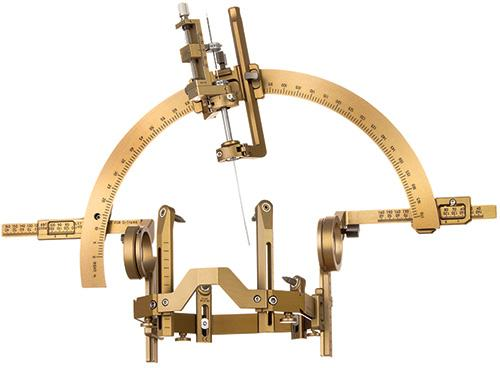
\includegraphics[width = 3.5in]{images/stereo_tactic_frame.jpg}
    \caption{A photograph of an example stereotactic frame that could be used for interventions and treatments during minimally invasive neurosurgery. \cite{stereotactic}}
    \label{fig:stereotactic}
\end{figure}


\section{Robotic Solution}
A potential alternative to manually aligning stereotactic frames for tool insertion is to achieve the same motion control with a robotic system. Such a system could obtain the tool location using the forward kinematics of the robot, registration of the robot to the imaging system, and MR images of the probe to precisely position the ablation tool at the treatment site. This promises significant speed and reliability improvements over manual tool alignment. Past research at WPI AIM Laboratory produced a five DOF neuroablation robot, called the neurobot, which was MRI compatible, lacking ferrous material, and did not distort the image significantly while operating its piezo electric motors to move. \cite{aimLabRobot} Kinematically, the system produced Cartesian translation from the base and orientation through a remote center of motion, emulating the workspace of stereotactic frames. Newer iterations of this system provide two extra degrees of freedom for the robot to perform the needle insertion along the insertion axis and to rotate the ultrasonic probe to enable more precise coverage of tumors once the probe is inserted. \cite{neurobotIros} \autoref{fig:neuroRVizModel} shows the latest version of the robot as a SolidWorks model.

\begin{figure}[thpb]
	\centering
	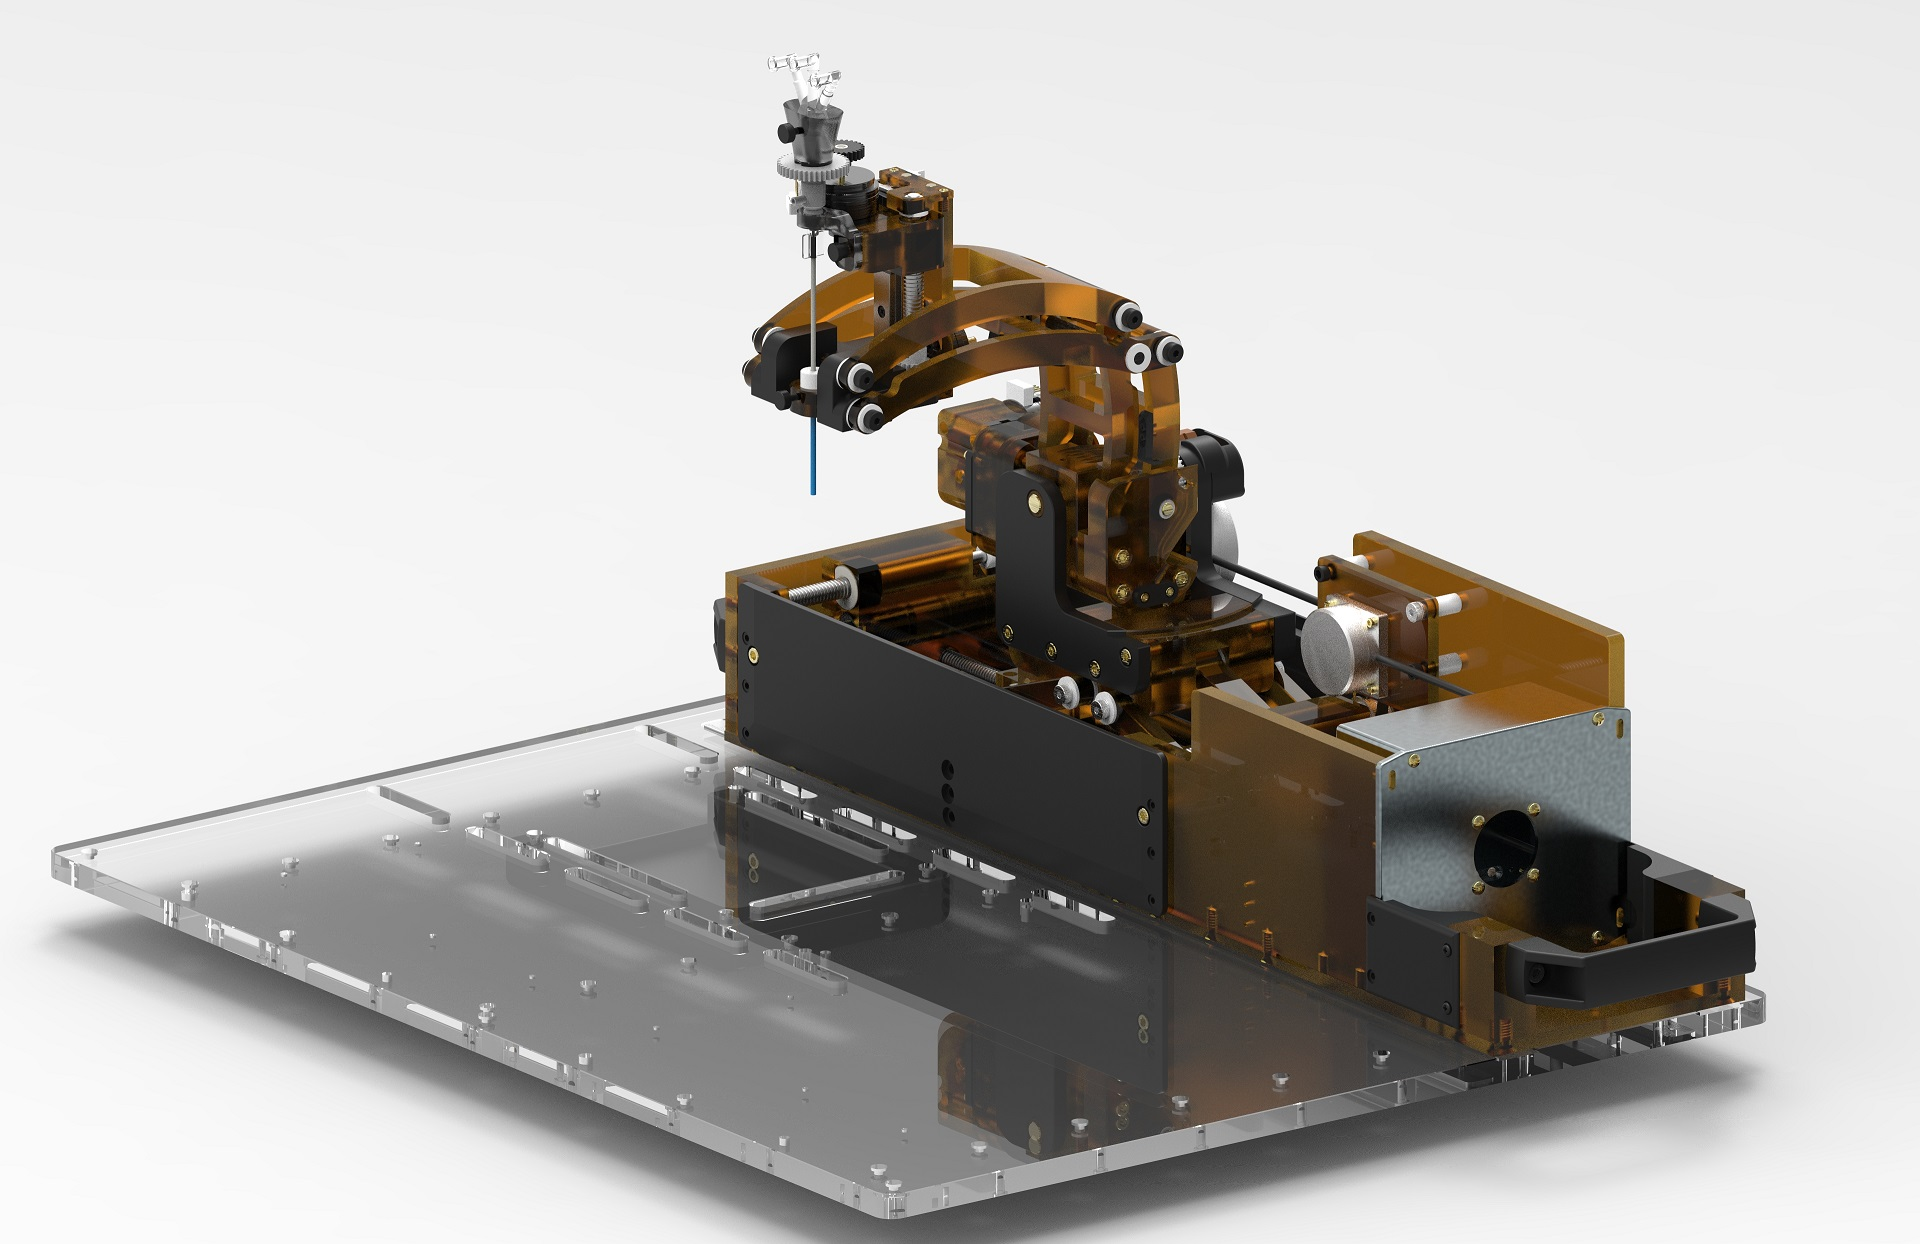
\includegraphics[width = 4in]{images/NeuroRobot_complete_26_reduced.jpg}
    \caption{Rendering of the Neurobot SolidWorks model. From \cite{neurobotIros}}
    \label{fig:neuroRVizModel}
\end{figure}


\section{Problem Description}
\label{sec:problemDescription}
As discussed earlier in \autoref{sec:clinicalProblem}, some of the primary challenges when working with minimally invasive surgical techniques are perception and maneuverability limitations. For the neurobot, these problems manifest themselves in two primary manners: 1) - it is difficult for operators to plan procedures with the robot without knowing what it can reach and 2) the robot needs to be able to move to the procedure location without striking obstacles. In other words, it is necessary to know where the robot can reach and how to move it there, and there are some complications of solving these seemingly simple problems. 

\subsection{Differentiation from Related Work}
Other work has focused on motion planning in MRI machines as a control problem by steering needles in soft tissue, \cite{needleSteeringSoftTissues} modeling needles as serial chains for conducting motion planning in task space, \cite{taskSpacePlanning}, and conducting workspace design analysis to optimize the robot's designed workspace within the MRI bore. \cite{prostateWorkspaceDesignAnalysis} \cite{workspaceOptimization} These works are associated with the topics in this one but do not provide a solution for analyzing the workspace in real-time by checking collisions with the scanner based on operative registrations. Motion planning techniques in the literature specialize in trajectory following for needles typically used in MRI as these holonomic problems are challenging to solve and the needle dynamics are complicated, but conventional rigid body manipulators do not appear to have been studied for workspace analysis and use in MRI scanners. Thus, this work seeks to develop a generic framework and approach for conducting workspace analysis and motion planning for a manipulator confined to an MRI scanner, yet apply this framework specifically in an implementation targeted for the neurobot while allowing for the possibility of adaption to other platforms. 

\subsection{Workflow Overview}
Current neuroablation procedures using the neurobot have a generally straightforward workflow for performing ablations, which is outlined below:

\singlespacing
\begin{enumerate}
\item Take preoperative images of the patient head.
\item Attach robot to scanner bed.
\item Register robot in MRI scanner. Extract scanner bed from bore.
\item Drill burr hole in skull for access to target site.
\item Secure patient on scanner bed and insert into bore.
\item Perform operative imaging of the patient.
\item Surgeon selects entry and target points.
\item Robot moves to entry point.
\item Cannula then probe inserted into patient with the robot.
\item Scanner bed inserted back into scanner.
\item Ablation treatment performed, repositioning and repeating as necessary
\end{enumerate}
\doublespacing

In the future, Step 4 of the workflow could be performed using the robot itself later in the workflow by equipping it with a drill, while in the current iteration, the surgeon completes the drilling. It would be ideal for the burr hole location to be chosen so as to optimize the robot's manipulability around the target zone, and having the robotic system inform this selection process and perform the drilling can further improve the workflow and procedure outcomes.

\subsection{Potential Problems in the Workflow}
Once the neurobot is attached to the patient table on the MRI scanner (Step 2), it faces several constraints that can interfere with achieving the desired needle insertion into the patient's head to place the ultrasonic probe at the treatment location (Step 9). Some of these are inherent due to the robot design itself while others are environmental constraints. A few of the robot's joint limits change based on the motions of other joints (i.e. the amount of axial travel depends on the current height due to a parallelogram/scissor lift mechanism). This complicates the modeling of the robot's kinematics in conventional robotics software packages and means that extra precautions must be taken when planning its motions and ensuring treatment locations are reachable.

Concerning the environment, there are two primary objects the robot and its end effector and attached instrument can unintentionally collide with and must avoid: the patient and the scanner. When the patient is secured on the scanner bed (Step 5), the robot must move to the entry point in the skull without striking the patient's head (8). This is aided by removal of the ultrasonic probe and cannula, as shown in \autoref{fig:neuroRVizModelNoProbe}. 

\begin{figure}[thpb]
	\centering
	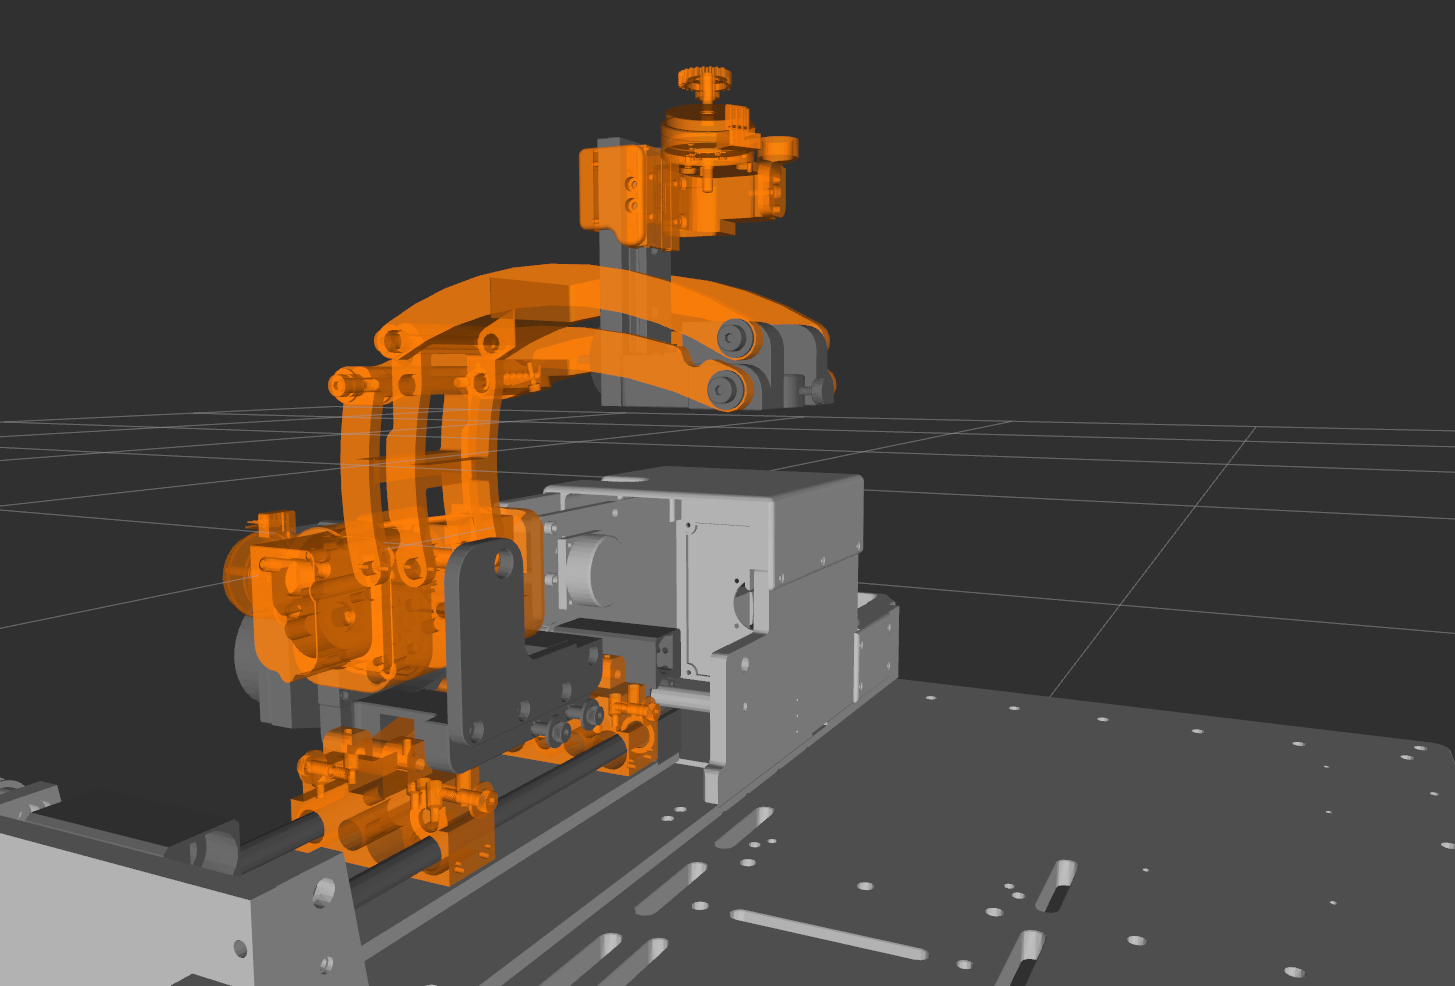
\includegraphics[width = 4in]{images/neuro_no_probe.png}
    \caption{Screenshot of RViz model of neurosurgical ablation robot in the configuration for positioning probe to entry point with the cannula and ultrasonic probe removed. }
    \label{fig:neuroRVizModelNoProbe}
\end{figure}

Once the robot is in place above the burr hole, the cannula is inserted into the skull and attached to the robot, and the ultrasonic ablation probe is attached to the robot and inserted into the brain by the robot's needle driver joint (Step 9). This final robot configuration must then be able to enter the bore of the MRI scanner without the ultrasonic probe or robot collide with the scanner as the scanner bed is inserted back into the scanner bore (Step 10). Therefore, a successful insertion solution must abide by the robot's kinematic limitations, avoid collisions with the patient's head and skull during movement along a trajectory from the starting configuration to the final configuration (with the cannula and probe removed), has a final configuration that does not collide with the MRI bore, and reaches the target destination successfully.

To meet this need currently, the neuroablation robot requires the coordination of two engineers to drive the robot joint-by-joint to prevent collision with the patient head and align the system to the desired insertion point. This process is time consuming and requires knowledge of the robot's kinematic limitations, increasing the difficulty for medical professionals to perform this procedure themselves. Further, the workspace of the robot is not visualized before the alignment is attempted. Given the placed burr hole in the skull, it would be very useful to know where the robot can reach and administer treatment, but this ability has not yet been realized. This limitation can lead to costly situations in which time is wasted attempting to align and reach a position that is outside the robot's workspace, in which case the patient may need to be repositioned and the workflow repeated.

\section{Contributions}
This project entails developing a research-grade software system which integrates existing medical platforms, provides a mechanism for evaluating the neurobot's reachable workspace, and generates collision-free trajectories to enable faster, less tiresome, and more intuitive surgical procedures using the neurobot in ultrasonic ablation with flexibility to be adapted on similar platforms. The specific contributions of this work include:

\begin{itemize}
\singlespacing
\item Designing and implementing a software system for conducting motion planning
\item Modeling the neurobot in and interfacing it to the ROS environment
\item Generating the collision-aware workspace of the robot
\item Computing the collision-aware treatment workspace given an entry point
\item Computing collision-free trajectories to control the robot's motion
\item Utilizing ROS-OpenIGTLink-Bridge to transfer data between the robot, software system and slicer
\item Employing 3D Slicer to visualize and interact with the generated data
\item Evaluate system performance on the neurobot
\item Demonstrate the system in animal trials
\end{itemize}

Known techniques from both medical and robotics fields are applied into this integrated system to produce a significant contribution for the problem described in \autoref{sec:problemDescription}. This work does not introduce a novel approach for motion planning or way of interfacing medical devices. Rather, it is an exercise in using current state of the art software within a new research-grade system to produce useful functionality with reduced development overhead. The utilized toolsets are also evaluated to perhaps illuminate some problem areas or technical stumbling blocks for other researchers wishing to accomplish similar objectives. In the end, this work advances the capabilities of the neurobot, making it easier to operate in the hope of improving surgical procedures and the outcome for patients suffering from cranial diseases.


%%%%%%%%%%%%%%%%%%%%%%%%%%%%%%%%%%%%%%%%%%%%%%%%%%%%%%%%%%%%%%%%%%%%%%%%%%%%%%%%
\chapter{Background and Related Work}
As a project that spans several technical fields, there are a number of topics that need further examination to better understand the current state-of-the-art and how this project relates to those developments. In this section, current medical technology, neuroablation procedures, the Neurobot platform, robotics tools including ROS, and motion planning concepts will be explored before the system design is discussed.

\section{Medical Technology}
The medical field has several key technologies that are closely entwined with the contributions of this project. This includes ultrasonic ablation, MRI, and medical imaging software tools.

\subsection{Ultrasonic Ablation}
\label{sec:ultrasonicAblation}
The process of ablating, or removing, tissue can be achieved through different means, with heat being one option in a process known as thermal ablation. \cite{thermalAblation} Ultrasonic thermal ablation involves utilizing ultrasonic energy to heat up surrounding tissue to the point at which it dies while leaving healthy tissue at safe temperatures due to the narrow field of applied ultrasound. \cite{thermalAblation} Once tissue has been exposed to high enough temperatures for a certain length of time, as shown in \autoref{fig:thermalAblation}, tissue will experience necrosis, or death. \cite{thermalAblationFocusedUltrasound}

\begin{figure}[thpb]
	\centering
	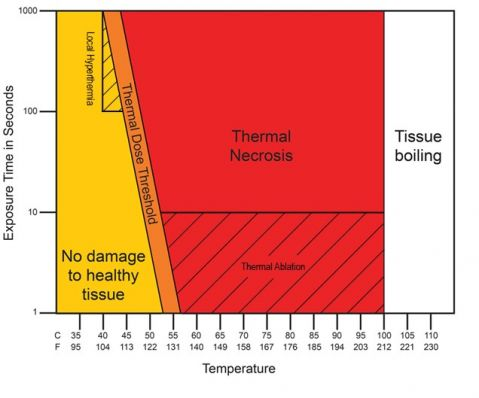
\includegraphics[width=4in]{images/Thermal_Ablation.jpg}
    \caption{Graph of tissue reaction to heating at particular durations of time. From \cite{thermalAblationFocusedUltrasound}.}
    \label{fig:thermalAblation}
\end{figure}

By modulating the length of time and exposure to temperatures, a very precise treatment (assuming sufficient monitoring and control) can be achieved which leaves healthy tissue unexposed to dangerous temperature levels for long lengths of time while fully destroying unhealthy tissue. The key to attaining this ideal treatment is through the monitoring process, which can be attained through MRTI, discussed in \autoref{sec:mrti}.

As previously mentioned, ultrasonic energy can be administered externally or internally to the patient. Outside of the patient, the ultrasonic beam is focused to a particular depth such that the focused energy of the ultrasound traveling through the body heats the target tissue to the point of necrosis, and this technology is known as High Intensity Focused Ultrasound (HIFU). \cite{hifu} Inside of the patient, ultrasonic treatment can be delivered through an element placed on a catheter or needle, referred to as interstitial ultrasonic ablation, and this method can provide conformal tumor coverage. \cite{interstitialAblation} By conducting a series of interstitial ablations, using different ultrasonic probes with limited fields of effect, or by rotating a probe with a non-symmetric ultrasonic beam, arbitrary tumor shapes and sizes can be effectively ablated. Planning and conducting these probe rotations and insertions to achieve proper treatment coverage is a goal of current research, and MRI provides a key mechanism for enabling that monitoring capability. Ultrasonic probes are typically MRI-compatible and cooled with water, which can increase their size due to piping, as shown in \autoref{fig:ultrasonicProbe}.

\begin{figure}[thpb]
	\centering
	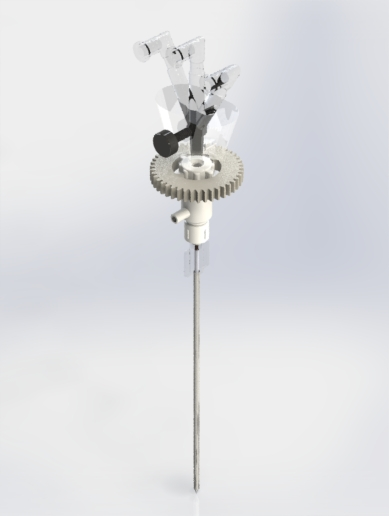
\includegraphics[width=3in]{images/ablation_probe_render.jpg}
    \caption{A SolidWorks render of the ultrasonic probe used in thermal ablation on the neurobot.}
    \label{fig:ultrasonicProbe}
\end{figure}


\subsection{Magnetic Resonance Imaging}
Magnetic resonance imaging (MRI) is a non-invasive imaging technique which utilizes a very strong magnet and radio frequency to image soft tissues in the body, providing 3D images when slices are combined together. \cite{mri} Essentially, hydrogen protons are spin-aligned to the magnetic field in the scanner, and radio waves are used to temporarily realign the protons while the radio is on. When the radio is turned off, the protons realign with the permanent magnetic field, releasing energy as they do so, and sensors in the scanner can resolve this energy release into 3D positions within the scanner. Based on a number of factors, differences in tissues (usually molecular density including water) can be detected and seen in the MR images, as seen in the image of the pig brain in \autoref{fig:mriPigImage}. 

\begin{figure}[thpb]
	\centering
	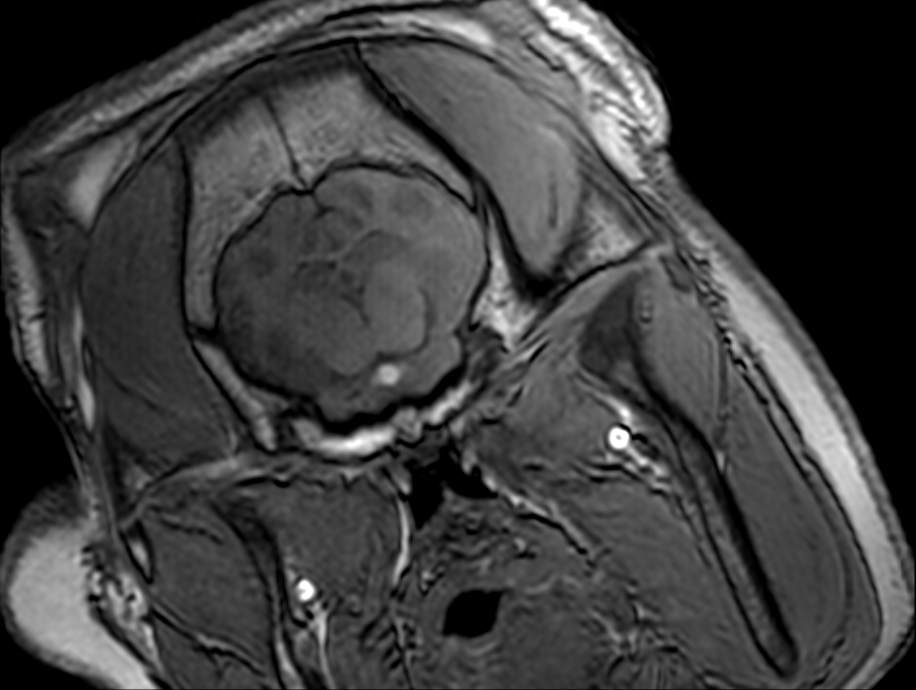
\includegraphics[width=4in]{images/MRI_scan_pig_brain.png}
    \caption{Example MRI image of a pig head, showing the brain and surrounding tissue.}
    \label{fig:mriPigImage}
\end{figure}

Because MRI's soft tissue contrast is much higher than X-Ray or CT scans and there is no ionizing radiation emitted (which can cause harmful DNA mutations), it is a preferred imaging method, yet more expensive, for cases where repeated images need to be taken to guide procedures. However, the tight confines within an MRI scanner (most are between 55-70cm in diameter \cite{mriSize}) makes scanning patients sometimes challenging and also hinders efforts to conduct medical interventions within the scanner. 

The scanner located at the UMASS Memorial Medical Center, the primary location for current tests with the Neurobot, is a Phillips Achieva 3T scanner with a 60 cm bore. 

\subsubsection{Frame Conventions}
MRI scanners typically follow the ISO Standard for frame conventions, which describe the orientation of images and the patient position within, as \autoref{fig:mriScannerFrame} illustrates. \cite{isoStandardMRI}  While there are some specialized naming conventions for the patient (anterior and posterior, left and right, and superior and inferior), these are generally straightforward frame definitions. Within the scanner itself, due to the cylindrical nature of the bore, the terminology of lateral and axial motions describe movements in the x direction and z direction respectively. The neurobot utilizes the RAS convention, where right is positive x, anterior is positive y, and superior is positive z as shown in \autoref{fig:mriScannerFrame}.

\begin{figure}[thpb]
	\centering
	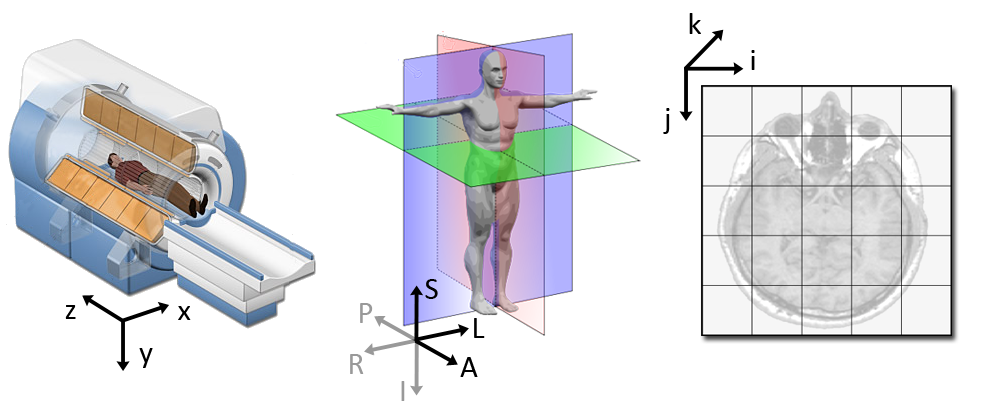
\includegraphics[width=\textwidth]{images/mri_coordinate_systems.png}
    \caption{Typical MRI scanner frame (left), patient frame naming conventions with the RAS convention used on the neurobot (center), and image pixel coordinate frame (right). From \cite{mriFrames}}
    \label{fig:mriScannerFrame}
\end{figure}

\subsubsection{Magnetic Resonance Thermal Imaging}
\label{sec:mrti}
MRTI is a scanning technique for MRI machines which effectively allows for real-time monitoring of changes in tissue temperature, which is of use particularly during ablation of thermal tumors in the body. \cite{mrti} This analysis can be conducted on a number of simultaneous or sequentially captured 2D slices in the MRI (either in parallel or orthogonal 2D planes) and serves great utility for monitoring the progress of thermal ablation procedures in that the ablation process can be terminated once the tumor tissue has received adequate heat so as to minimize damage to surrounding, healthy tissue. \cite{mrtiAblation} \autoref{fig:mrtiExample} shows an example of MRTI and tissue necrosis analysis on an ablation procedure.

\begin{figure}[thpb]
	\centering
	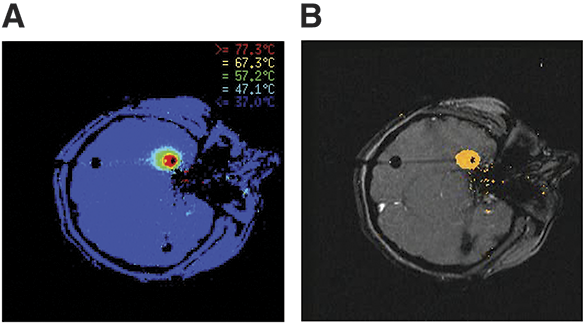
\includegraphics[width=4in]{images/mrti_head.png}
    \caption{A) Image showing temperature change as obtained using MRTI techniques during an ablation. B) The computed zone of tissue necrosis in the brain around the tumor. From \cite{mrtiAblation}}
    \label{fig:mrtiExample}
\end{figure}


\subsection{Medical Imaging Software}
While commercial MRI scanners typically ship with the manufacturer's own software solution for running the scanner and collecting and viewing images, there is a growing interest in providing open-source methods for analyzing MRI's without proprietary software and creating open standards for interfacing with devices. These two desires have been addressed by the development of OpenIGTLink and 3D Slicer, open-source software which has greatly assisted recent medical research.

\subsubsection{OpenIGTLink}
OpenIGTLink is a communications protocol which standardizes the interfaces of scanners, surgical systems, and analytical tools on computers. \cite{openIGTLinkPaper} \cite{openIGTLink} Essentially, this could do for the medical research world what ROS did for much of robotics research (see \autoref{sec:ros}). The specifications for the OpenIGTLink protocol allow equipment from different manufacturers to be compatible (or at least allow compatible drivers to be written easily) to reduce the overhead of researchers using these systems for planning, image collection, and image analysis. It supports real-time communications with data types specifically designed for and needed by medical imaging systems.

\subsubsection{3D Slicer}
3D Slicer is an open-source computer application for viewing and processing medical images. \cite{3DSlicerPaper} \cite{3DSlicer} It includes a large assortment of downloadable extensions from a repository contributed to by a growing community, and it is relatively straightforward to write custom extensions or modules in C++ or Python. The main goal of Slicer is to fulfill a need of researchers and the general public to have a free tool for accessing medical images and to serve as a platform for conducting experimental image processing and research for image-guided interventions. It includes an OpenIGTLink extension, which effectively allows it to interface with any OpenIGTLink-supported devices. The interface yields itself easily for interacting with imaging data and includes many processing techniques useful during pre-operative planning and during surgical procedures. \autoref{fig:3DSlicerScreenshot} shows a screenshot of the 3D Slicer application.

\begin{figure}[thpb]
	\centering
	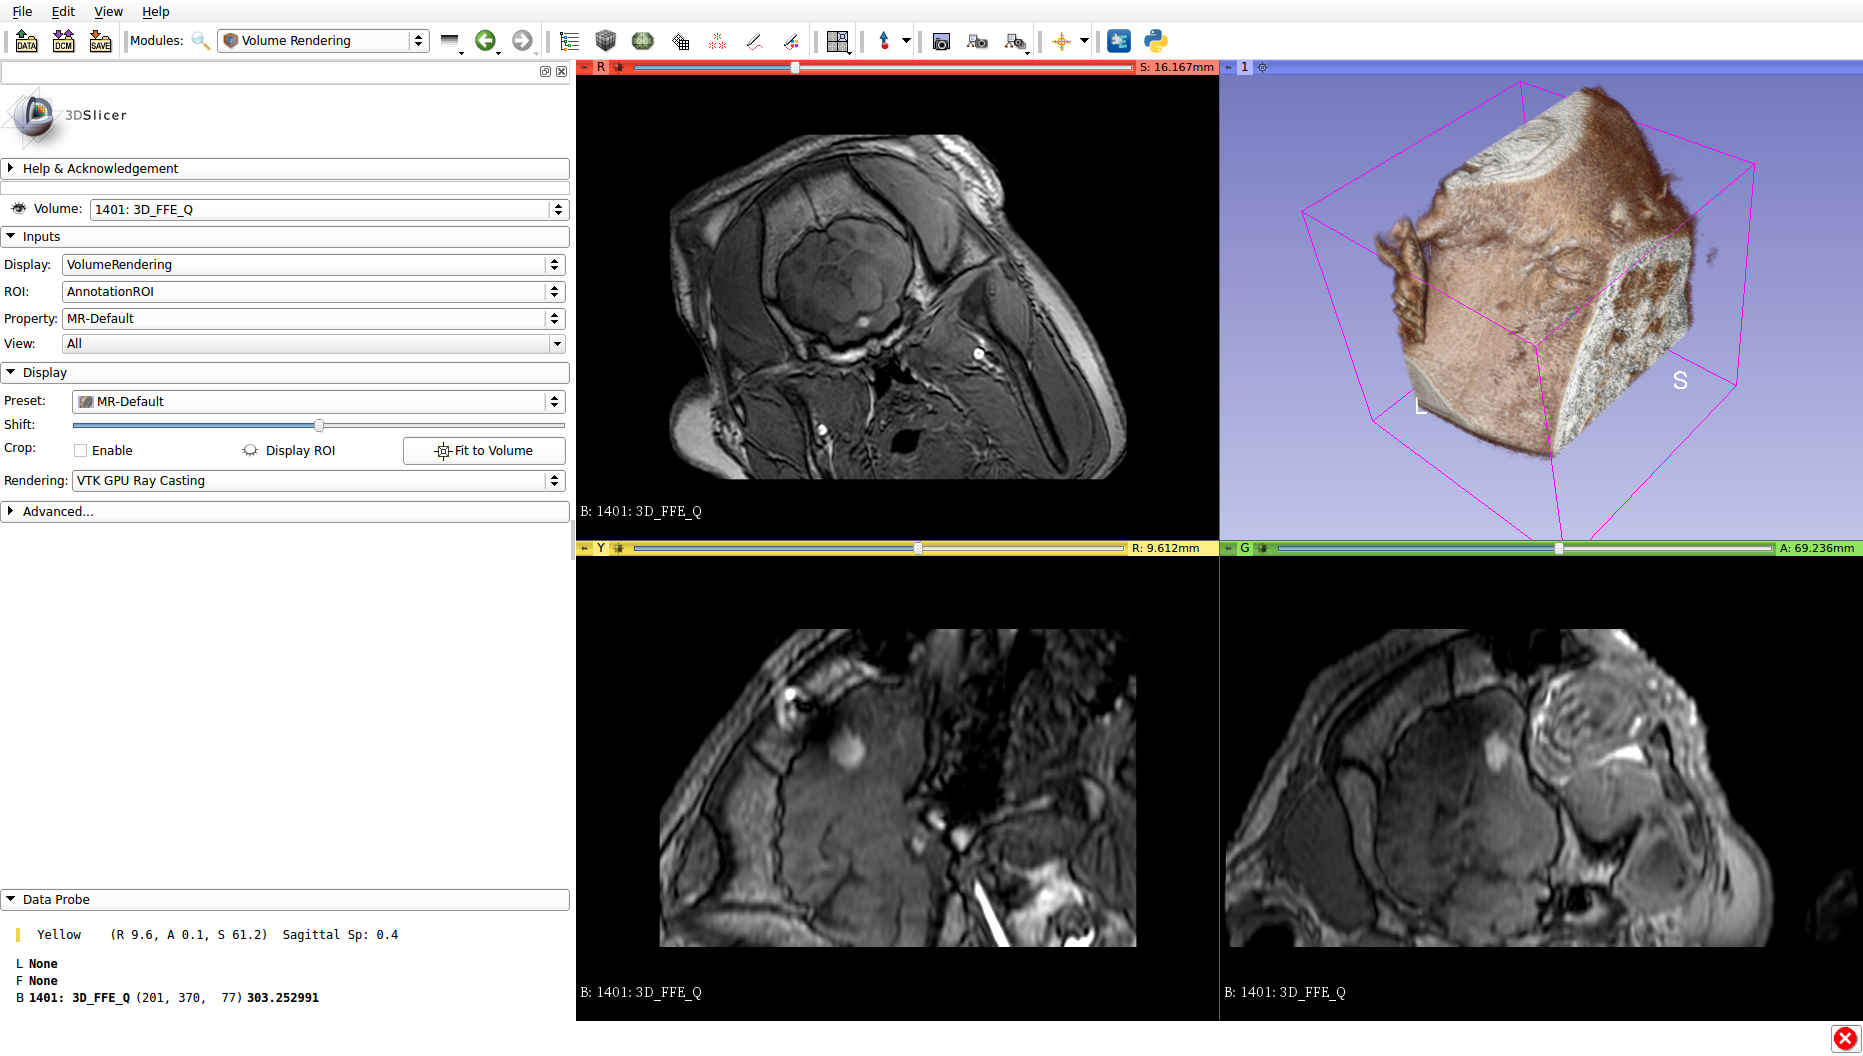
\includegraphics[width=\textwidth]{images/Slicer_screenshot_pig.png}
    \caption{Screenshot of 3D Slicer application being used to view MR images of a pig head with a volume rendering using ray casting in the top right corner.}
    \label{fig:3DSlicerScreenshot}
\end{figure}


\section{AIM Lab Neuroablation Robot Platform}
\subsection{System Overview}
The neurobot is a seven DOF robot with piezoelectric motors with encoder feedback shaped in a form factor capable of fitting within an MRI bore, as shown in \autoref{fig:neurobotRenderInTube}. As stated previously, the current iteration has stemmed from a series of developments in WPI's AIM Laboratory. \cite{aimLabRobot} Electrical components are designed to limit the noise introduced in the scanner environment, which can degrade the quality of MRI. This is especially apparent with the choice of motors; since most motors rely on magnetic fields to operate, traditional brushed or brushless motors cannot be used inside an MIR machine. Alternatives are available, such as pneumatic steppers and piezoelectric motors, which utilize piezo elements which flex under electrical voltages to achieve motion to drive shafts. \cite{piezoLegs} The mechanical components are iron-free and MRI compatible, which allows it to operate in the MRI freely, and it can undergo proper sterilization and covering procedures during surgery.

\begin{figure}[thpb]
	\centering
	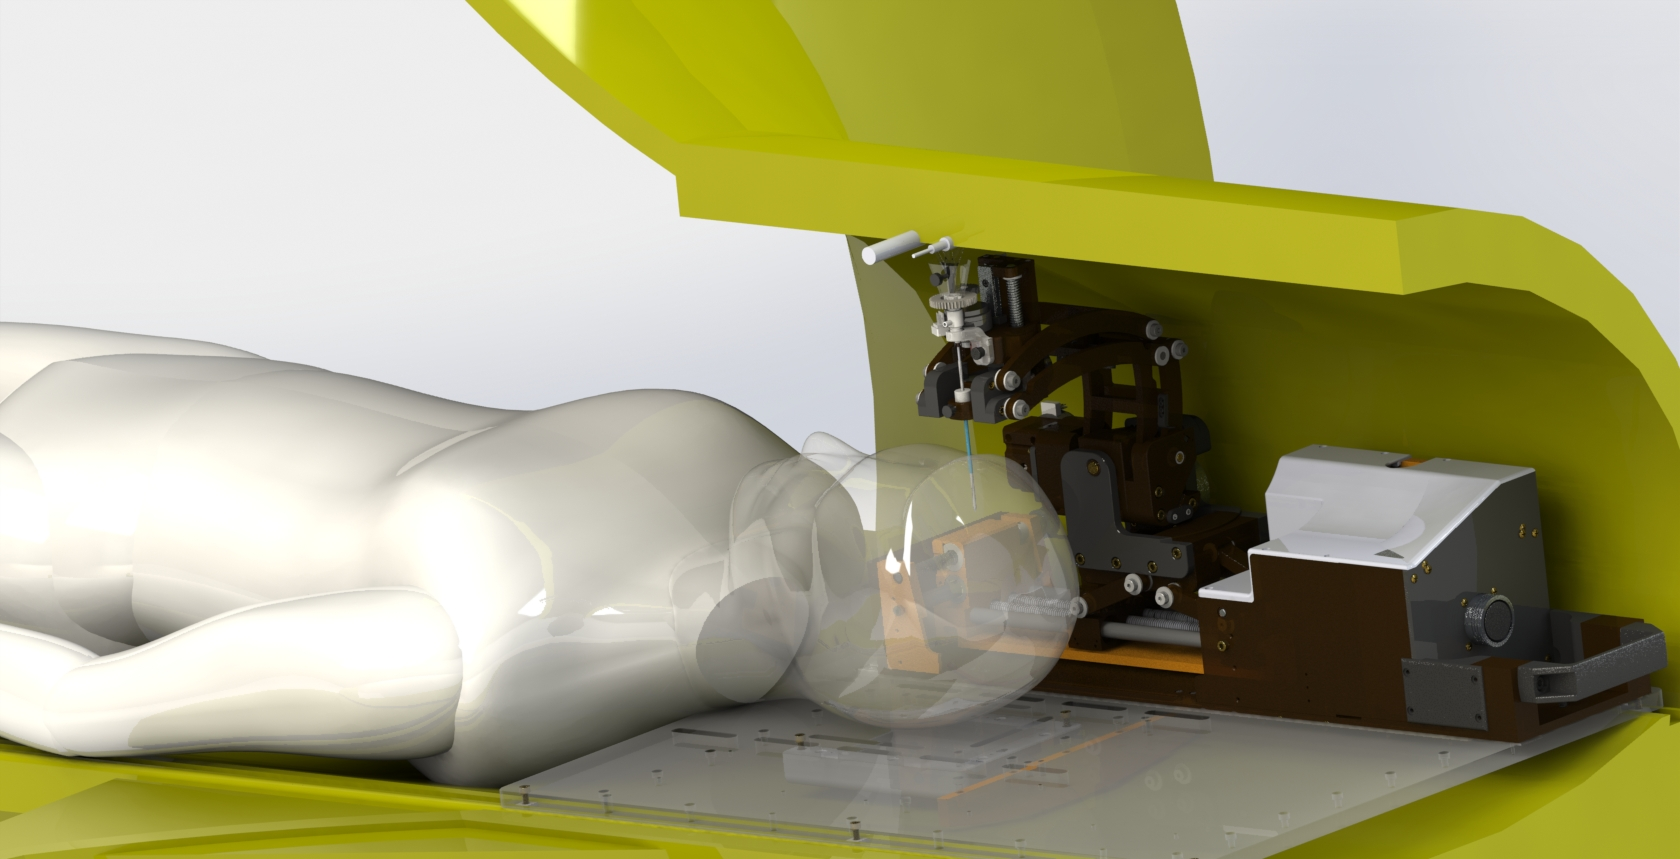
\includegraphics[width=4in]{images/neurobot_rendering_with_patient_in_bore.png}
    \caption{Rendering of neurobot SolidWorks model in cut-away MRI scanner bore.}
    \label{fig:neurobotRenderInTube}
\end{figure}

The robot is connected via a copper wire tether to a control box which resides in the MRI scanner room. Motor control boards and an embedded microprocessor with an FPGA provide the low-level functionality for the robot, including position control, safety features, and communications. WPI custom built most of the components in the interface box, and the system setup in the MRI console room is shown in \autoref{fig:networkDiagram}. The interface box is connected to a pneumatic safety foot pedal, which enables robot motion when the operator presses it, a fiber optic cable for communication, and a power cable to a standard 120 volt wall outlet. Only the fiber cable leaves the MRI scanner room through a barrier wall into the operator control room. Here, a computer can be connected to the robot to control it, and other computers interface with the MRI scanner to configure scans and obtain images. 

\begin{figure}[thpb]
	\centering
% 	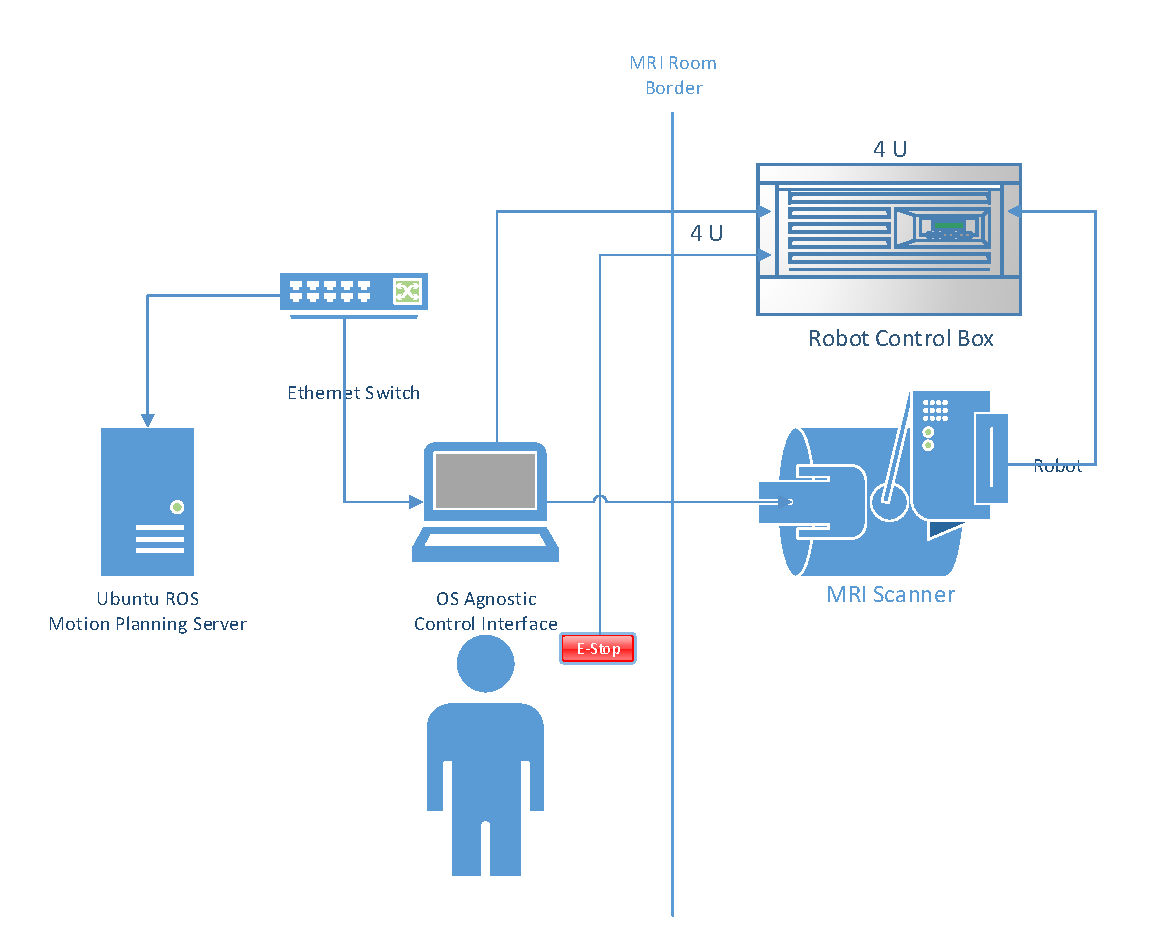
\includegraphics[width=4in]{diagrams/Networking_Diagram.pdf}
	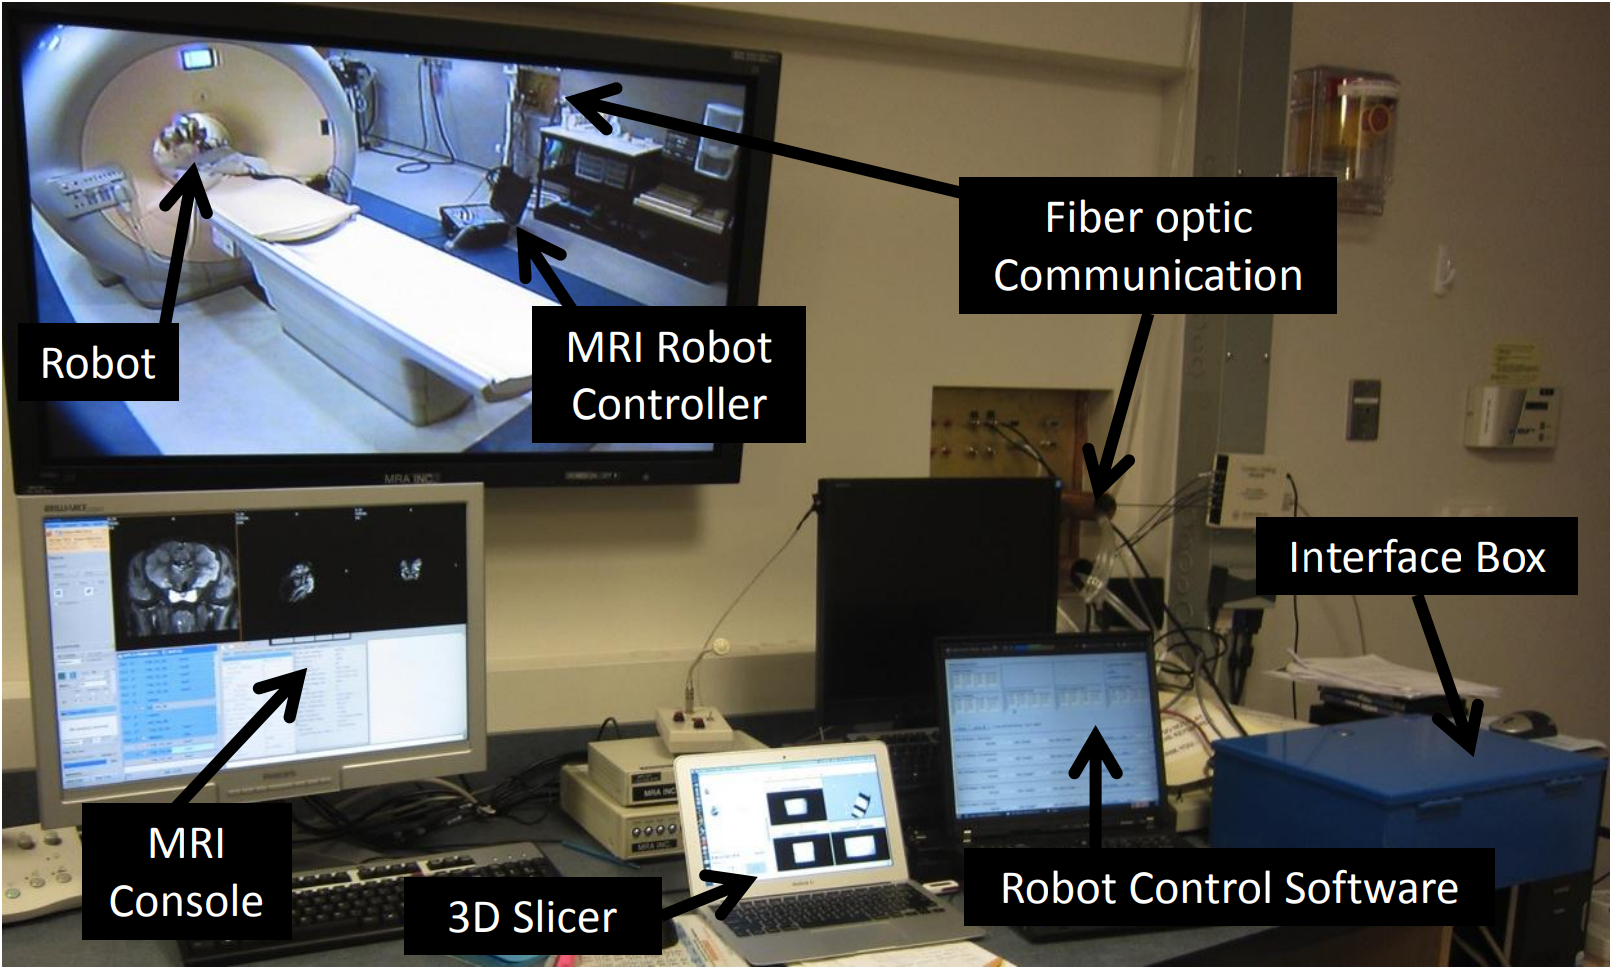
\includegraphics[width=4in]{images/mri_console_room.png}
    \caption{Photograph with annotations showing the interfaces between the robot, control computer, and MRI scanner in the console room. The computer monitor shows a camera feed from the scanner room on the other side of the wall. From \cite{neurobotIEEE2015}}
    \label{fig:networkDiagram}
\end{figure}

\subsection{Coordinate Frames}
Most of the neurobot frames follow similar conventions to those used in the scanner itself. \autoref{fig:neurobotFrames} show the primary coordinate frames of the robot: the tool frame and the base frame, which is defined by the z-frame attached to its base. The z-frame is a specially designed fixture for image-based registration in an MRI scanner. The structure holds vials of MRI-visible liquid at geometrically aligned locations in which performing image analysis on scans of the z-frame allow the centroid of the frame to be identified relatively quickly and accurately. \cite{zFrame} This z-frame then serves as the registration between the scanner frame and the robot. The optical frame of the scanner is simply a translational offset from the base frame. Since the robot is always situated in the scanner in the same orientation, movements in the base frame x direction are considered lateral and movements in the z direction are considered axial.

\begin{figure}[thpb]
	\centering
	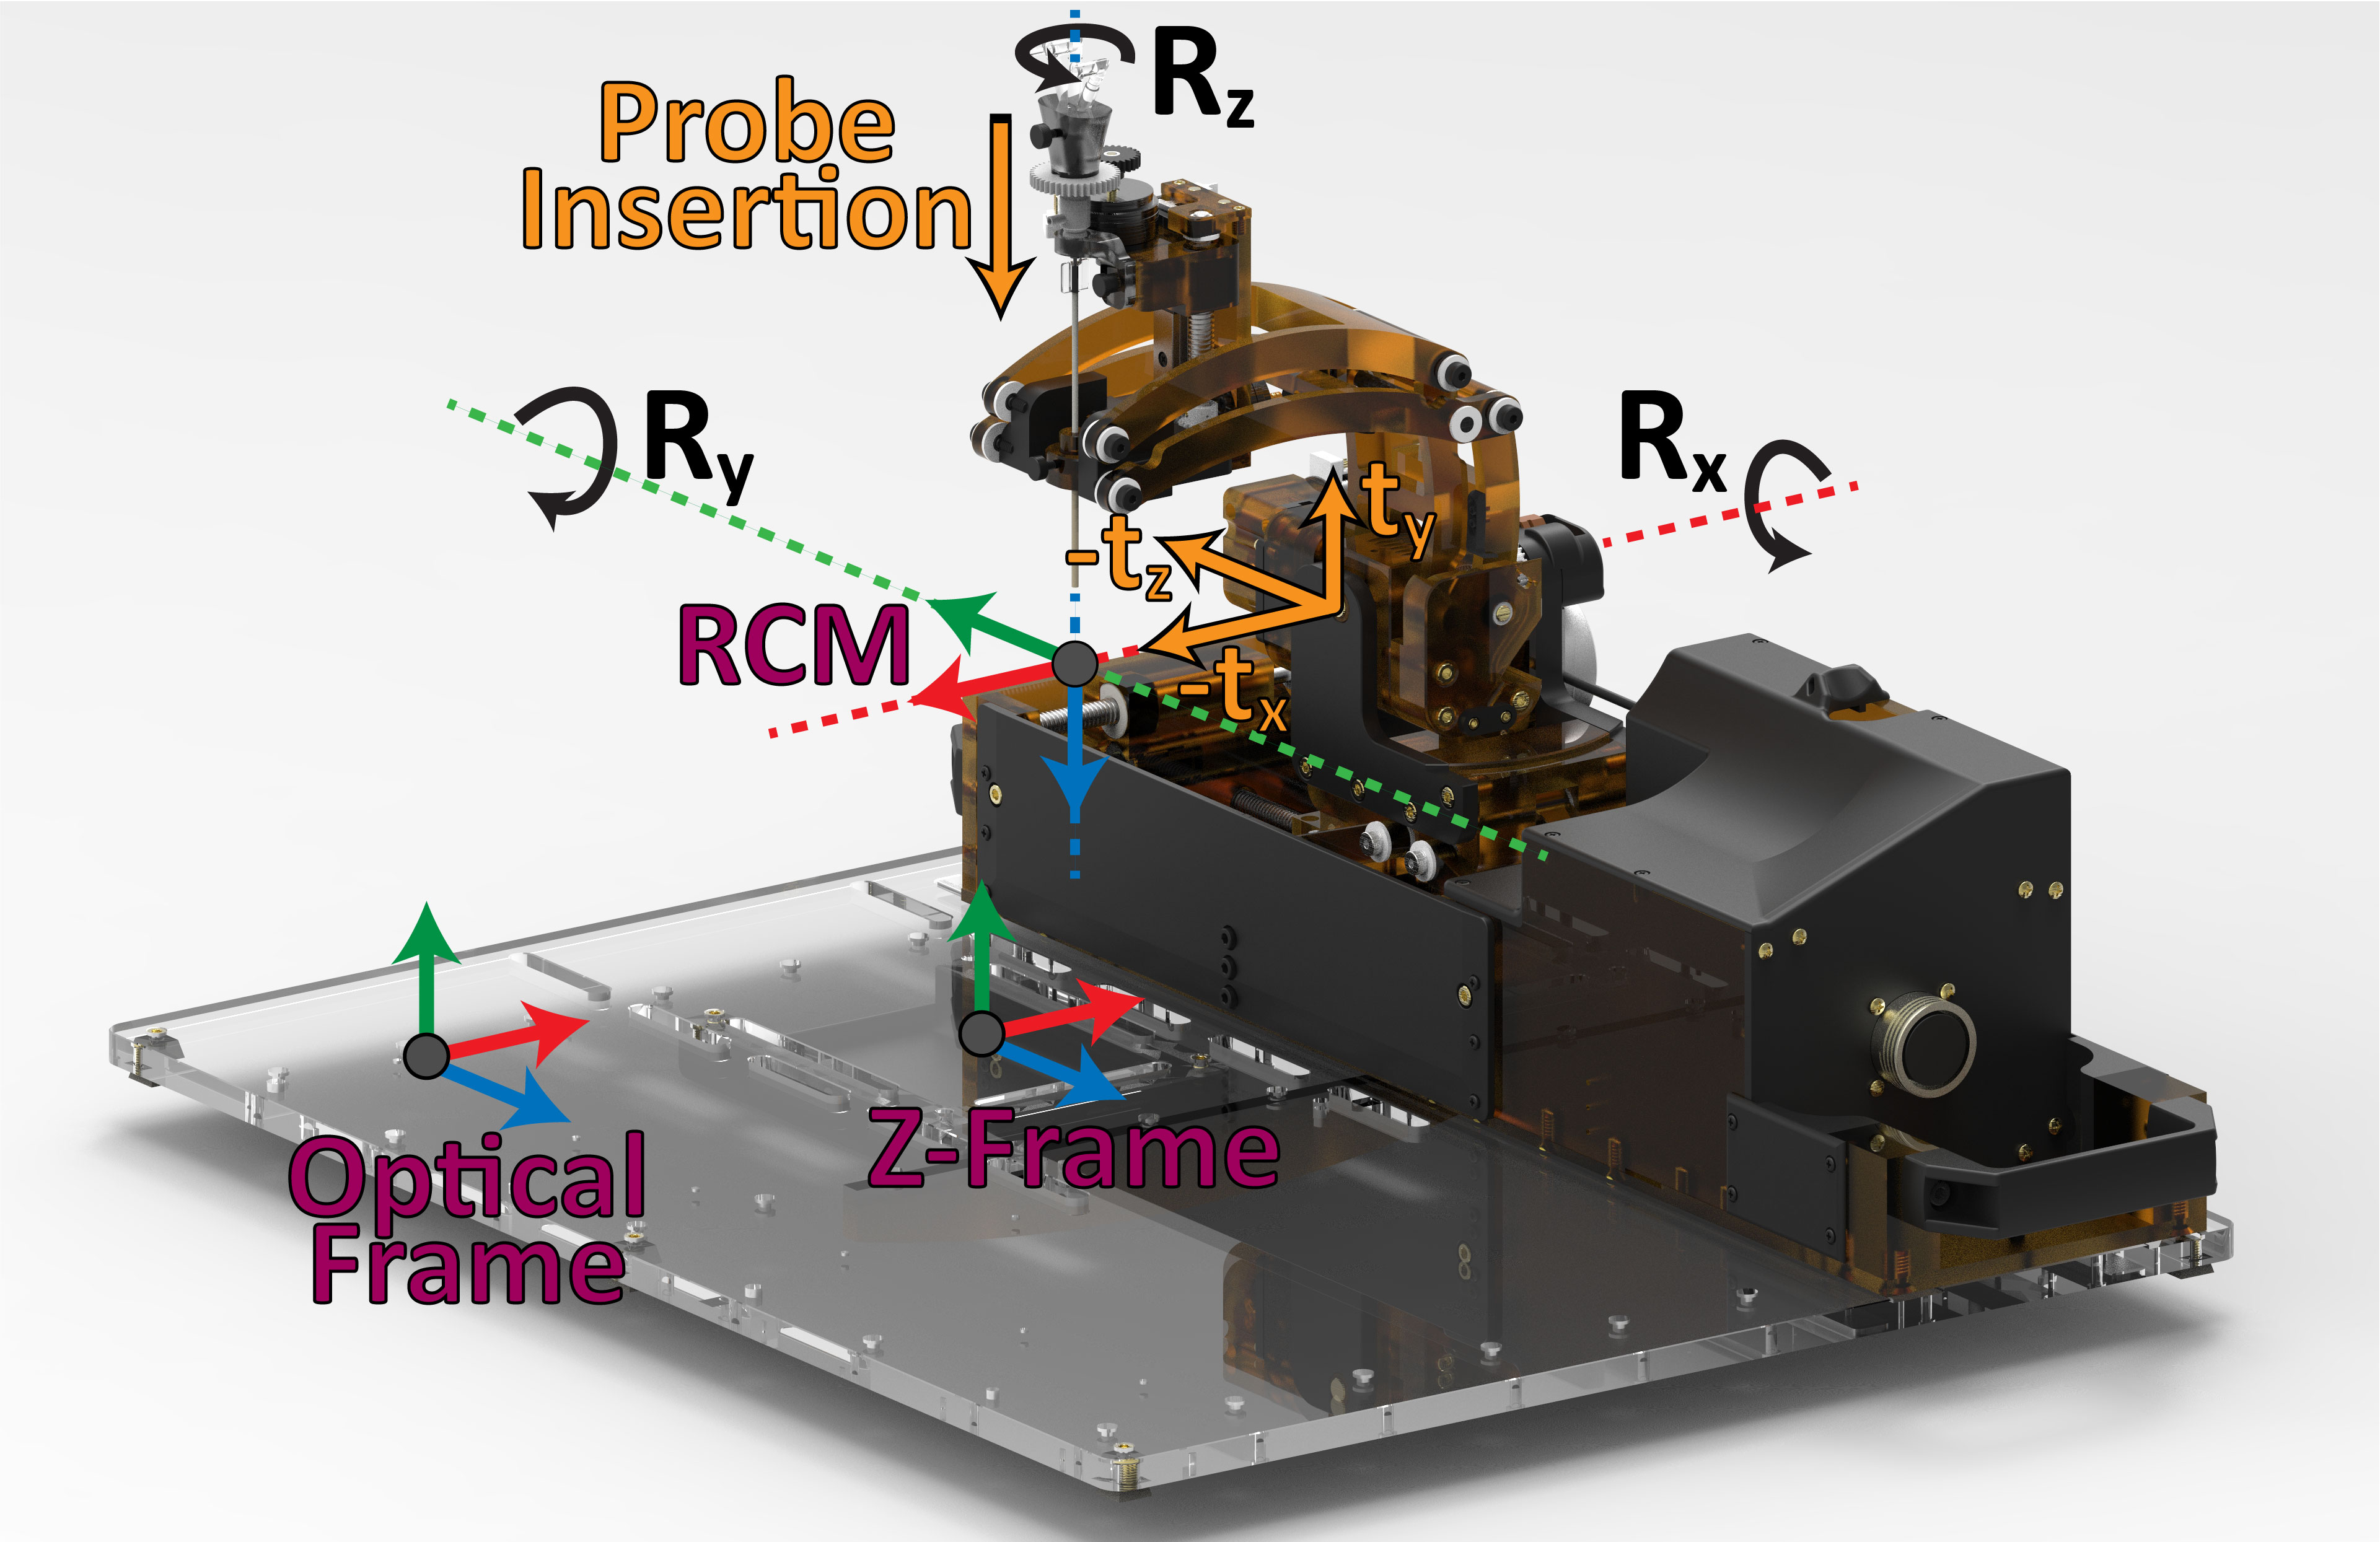
\includegraphics[width=\textwidth]{images/neurobot_frames.jpg}
    \caption{Neurobot frames and naming conventions. From \cite{neurobotIros}}
    \label{fig:neurobotFrames}
\end{figure}

\subsection{Kinematics and Joint Information}
\label{sec:kinematicsJointInfo}
The neurobot is essentially a Cartesian platform base with a remote center of motion wrist which also includes a degree of freedom for driving the needle along its axis, as illustrated in \autoref{fig:neurobotKinematics}, totaling seven active DOF. This makes the system under constrained in some configurations. Cartesian motions of the base are achieved through screw drives, with lateral translation being a simple screw driven joint. Vertical and axial motion is obtained through a differentially driven pair of lead screws attached to a parallelogram mechanism. When both screws are driven in the same direction, this achieves axial translation. When screws are driven in different directions, the `legs' of the parallelogram are brought closer together or further apart, which achieves a change in height.

\todo[inline]{Jane: Please add a DH parameter table to describe the forward kinematics of the needle insertion system.}

\begin{figure}[thpb]
	\centering
	%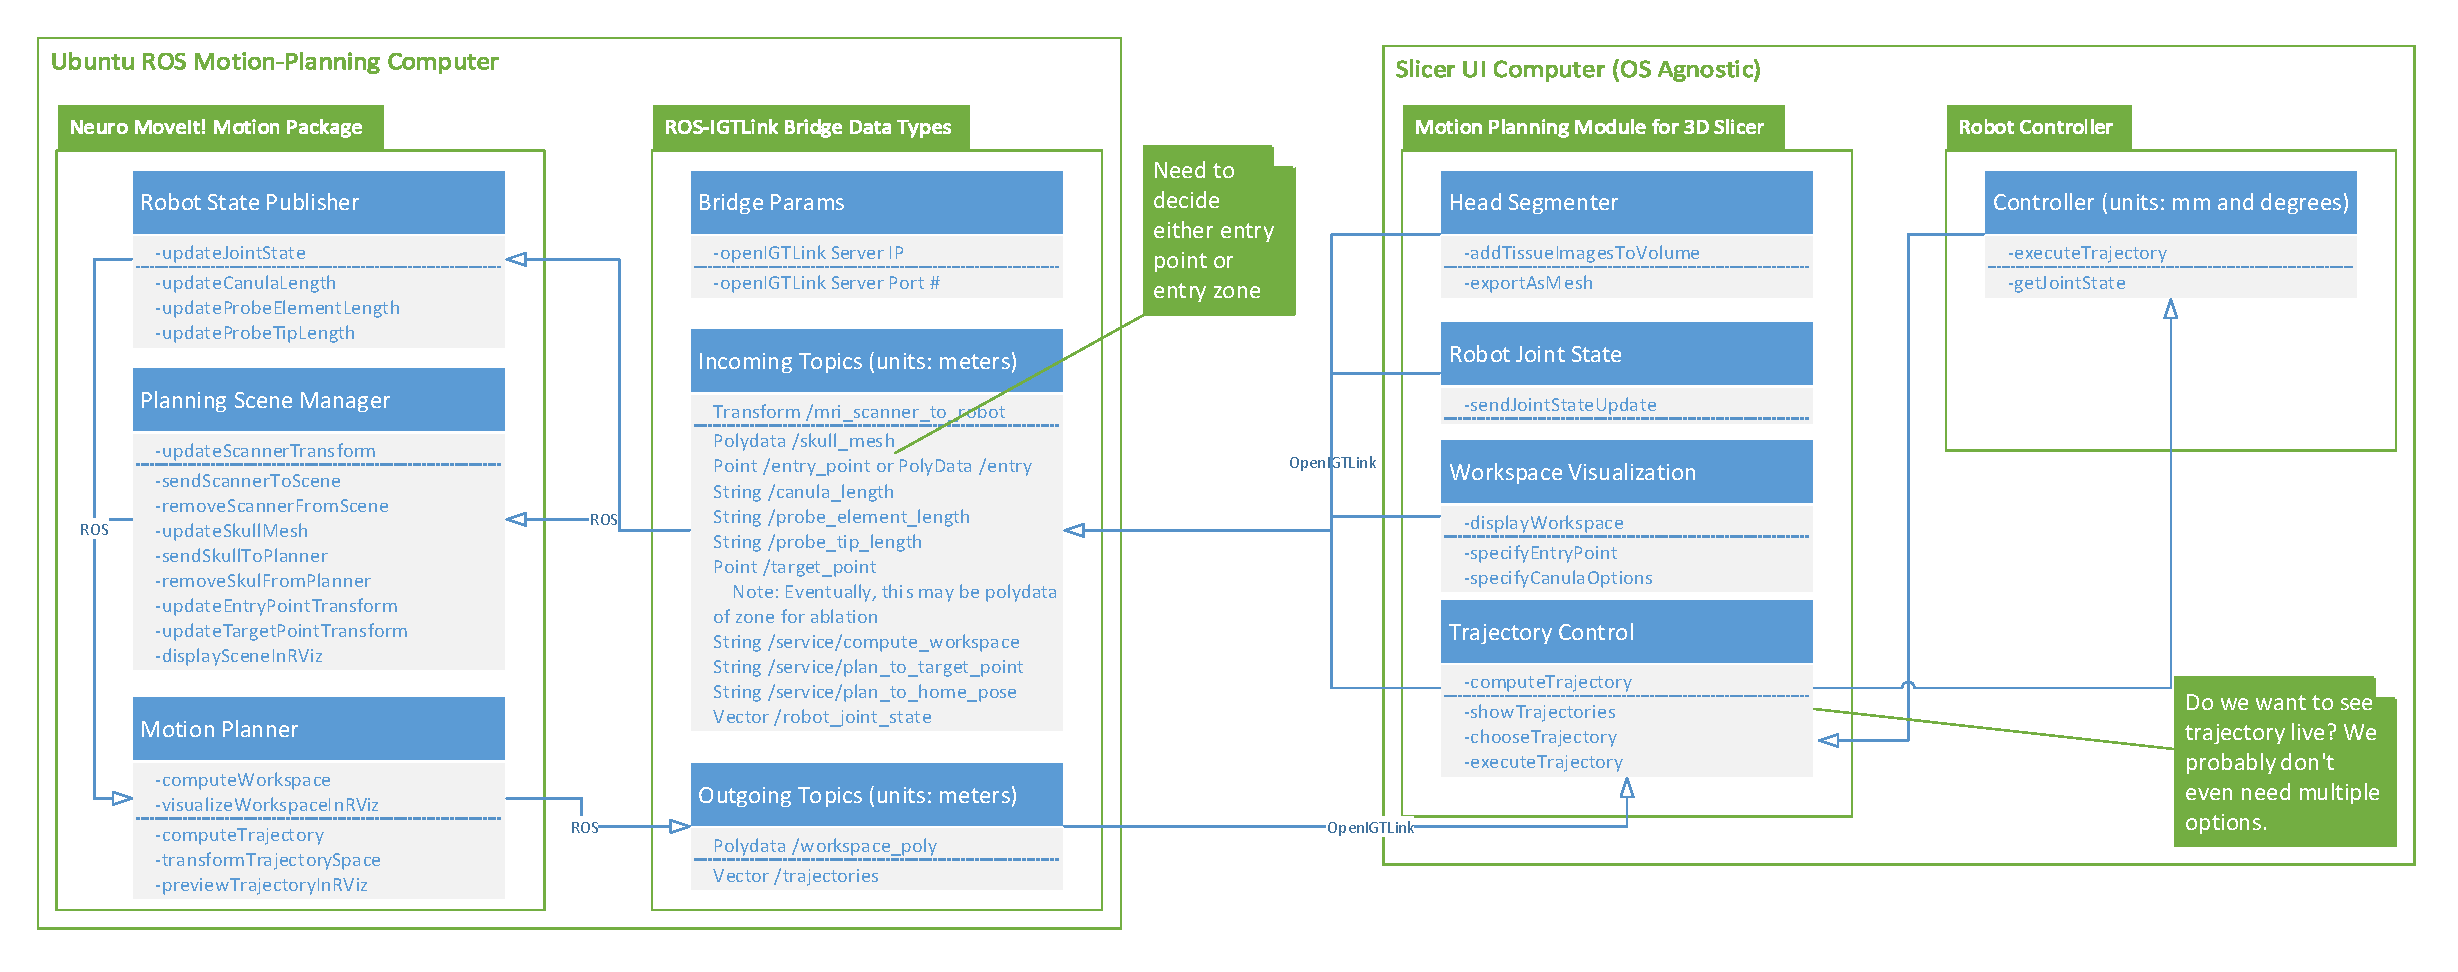
\includegraphics[width=\textwidth]{diagrams/Software_Diagrams.pdf}
    \missingfigure[figwidth=4in]{Neurobot kinematics, possibly from 3 views }
    \caption{Neurobot kinematic structure.}
    \label{fig:neurobotKinematics}
\end{figure}

Rotational motion of the upper assembly of the neurobot is attained through revolute joints. Changes in yaw are rendered by a single point of actuation to rotate the entire upper assembly. To achieve pitch changes about the remote center of motion, a linkage translates rotations at the base near the yaw joint to that about the RCM. The needle driver is a linear screw prismatic joint which can translate the needle through the hollow cannula a total travel depth of 4mm. Finally, a gearing at the top of the needle allows the needle to rotate continuously, useful for non-symmetrically beamed ultrasonic probes in order to aim the treatment appropriately. \autoref{tab:jointInfo} summarizes some more information considering the joints on the neurobot.

\todo[inline]{Include the equations used to formulate the FK and IK? GF: yes, please include annotated figures and corresponding equations that match what you used in your code}

\begin{table}[htbp]
\caption{Joint types and limits in position and velocity.}
\label{tab:jointInfo}
\todo[inline]{Double check these values with neuro team.}
% update with https://docs.google.com/document/d/136ywwUs2Z6RTJQrI72aEzYw0TrwOrAI5MM6YhfEL3f4/edit
\vskip6pt
\centerline{
		\begin{tabular}{|p{3cm}|p{2cm}|p{3cm}|p{3cm}|p{3cm}|}
		\hline
		\bf{Joint Name} & \bf{Type} & \bf{Lower Limit} & \bf{Upper Limit}  & \bf{Max Speed} \\ \hline
		Lateral & Prismatic & 0m & 0.055m & xx \\ \hline
		Axial 1 & Prismatic & 0m & 0.15m & xx \\ \hline
        Axial 2 & Prismatic & 0m & 0.15m & xx \\ \hline
        Yaw & Revolute & 0deg & -90deg & xx \\ \hline
        Pitch & Revolute & -35deg & 35deg & xx \\ \hline
        Needle Driver & Prismatic & 0m & 0.04m & xx \\ \hline
        Needle Rotation & Revolute & Continuous & Continuous & xx \\ \hline
		\end{tabular}
	}
\end{table}

\subsection{Software Control System}
Within the interface control box of the neurobot is an embedded system with a microprocessor running Linux and an FPGA board. This board runs the joint-level position control and calibration routines for the robot, reading in encoder data and interfacing with the piezo driver cards to properly drive the axis to the proper set points. The software computes forward and inverse kinematics for the robot and can publish and receive data over OpenIGTLink.

A web interface is used to control the robot over the fiber optic network interface. Joint level commands can be inputted using this interface and sent to the robot, and the IK solution can be used to specify a desired target position for the robot and drive the joints to that state. To resolve the desired position and orientation of the end effector for IK computation, the entry point in the skull and the treatment location are specified using the interface. From there, target joint values are set and the operator can enable or disable particular joints and press the foot pedal to begin motion.


\section{Neuroablation Procedures}
\label{sec:neuroablationProcedures}
Setup for a neuroablation procedure is fairly similar to other types of surgical procedures involving the brain and use of an MRI scanner. Preoperative images are usually taken of the patient to identify where the tumor (or planned treatment area) is located with respect to the patient's anatomy. Current tests with the neurobot are being conducted with live swine subject which are kept under general anesthesia. The surgeon places a burr hole, a small hole in the skull created using a special drill that stops at the brain matter, in the skull at a location they deem to be suitable through which to insert the ultrasonic probe and be able to reach the treatment site.

The robot is rigidly bolted to the MRI scanner bed after the scanner bed has been homed, and the z-frame registration is performed after the robot has homed itself and calibrated its joint encoders. Images are taken of the z-frame and then inputted into a computer running TheraVision which computes the registration using the fiducial vials in the z-frame. This registration is manually typed into the robot control software interface. The ultrasonic probe and cannula are removed from the robot, then the bed is backed out of the scanner and the patient is placed and strapped down. Once the patient has been imaged, planning for the neurobot ablation can begin.

As seen in \autoref{fig:offsetConventions}, there are four different offsets used by the control software to configure the parameters for solving IK for entering the patient head and reaching the treatment location with the ultrasonic element on the probe. These offsets are user adjustable for tailoring the solution for insertion to give a safety cushion around the patient and to simplify the problem of solving the IK for the robot.

\begin{figure}[thpb]
	\centering
	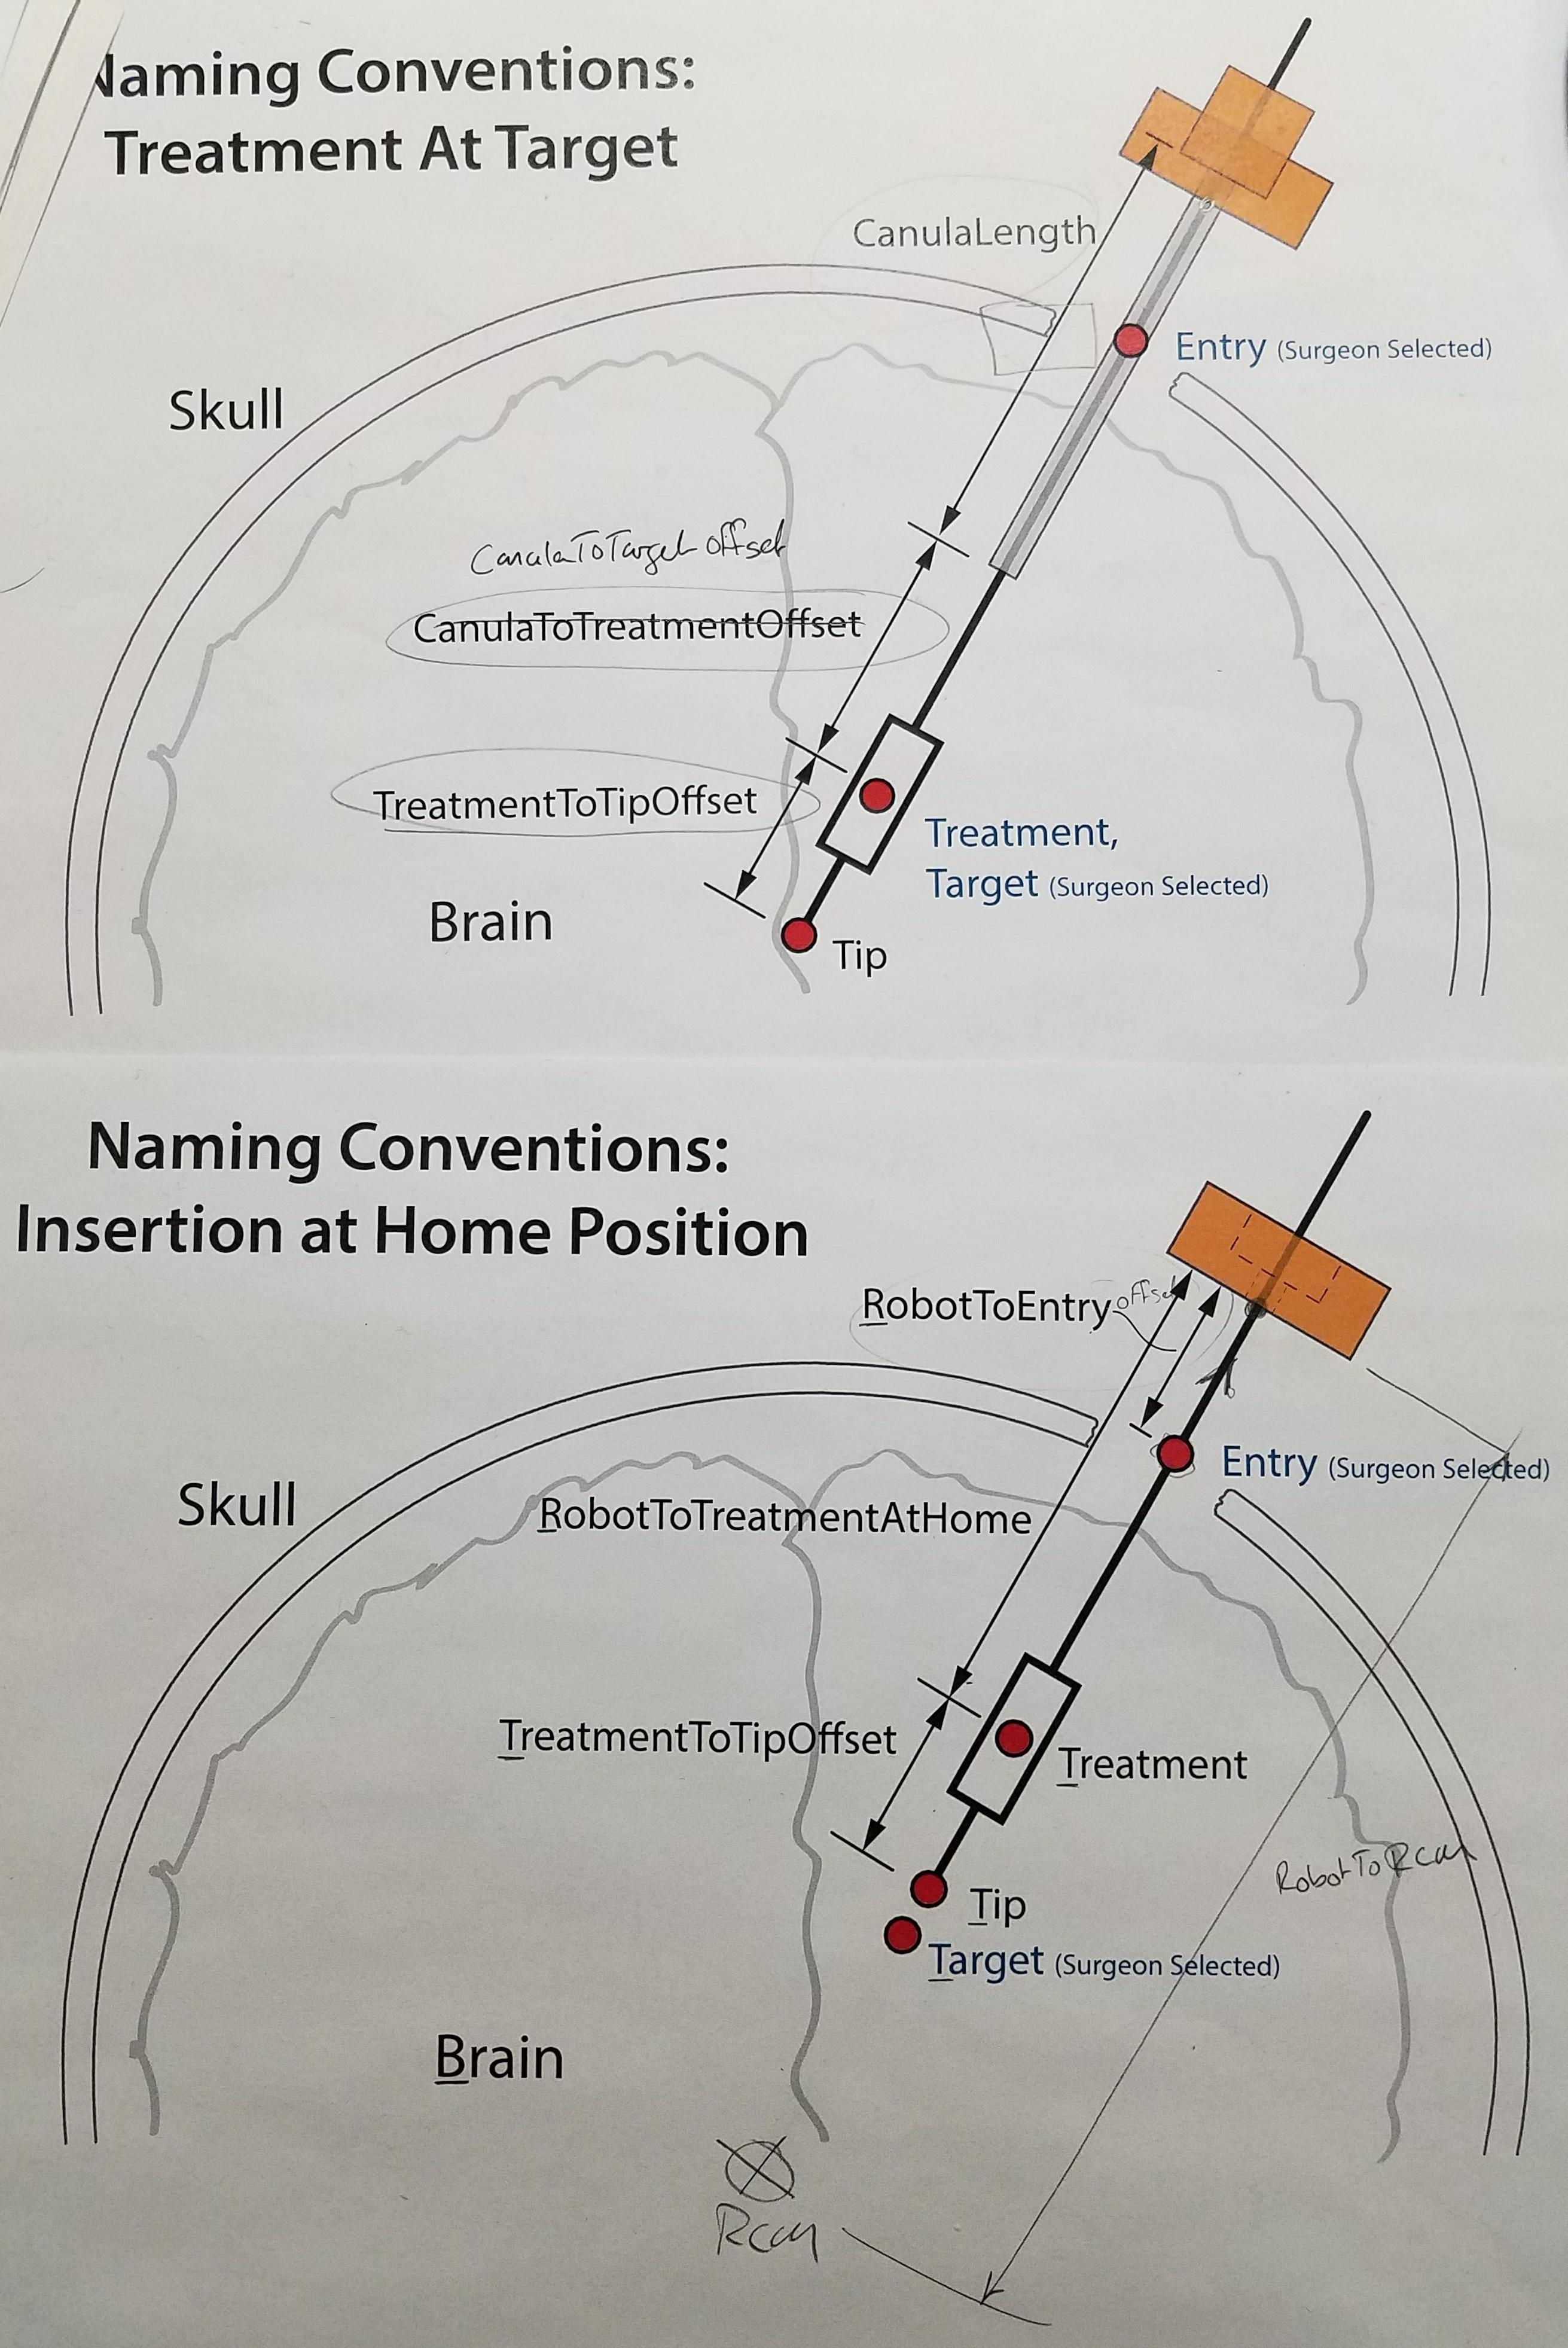
\includegraphics[width=4in]{diagrams/neuro_offsets_flip.jpg}
    \todo[inline]{GF: Get originals}
    \caption{Treatment offset definitions used by the robot control software. }
    \label{fig:offsetConventions}
\end{figure}

Without feedback for illustrating the workspace of the robot given the entry point on the patient, it is possible that when the surgeon selects an entry and target point on the patient using 3D Slicer that these do not resolve into a viable pose for the robot to reach the target. In the current procedure, the entry and target are input into the IK solver on the robot controller, and if it is unreachable, a new target is selected, the offsets can be adjusted, or the entry location can be varied slightly. If the pose is reachable, it does not guarantee that the robot or attached ablation probe will avoid collisions with the MRI scanner once the bed is inserted back into the bore. If this occurs, then the patient may need to be repositioned so that the entry point is in a more accessible location to reach the target zone with the neurobot.

\section{ROS Architecture and Tools}
\label{sec:ros}
The Robot Operating System (ROS) is a software platform officially supported on Ubuntu Linux which seeks to make developing robotics systems easier by standardizing sensor drivers and data types and providing common tools on which to build software for robotics systems. \cite{rosPaper} ROS is not an operating system by any means, but rather provides a node-based communication framework with standardized messages which are published and subscribed to using different topics. This allows a distributed system to be built relatively easily, with nodes unconcerned with what computer or robot is publishing data, and it also makes a system more abstract and modular. As long as, for instance, a sensor driver exists for publishing the standard ROS point cloud message for a certain piece of hardware, that hardware can be used as easily as any other and software becomes hardware agnostic. This reduces the amount of work the programmer must complete to get a new system running and greatly simplifies the ability for simulations to be performed with different platforms.

Apart from the libraries used to achieve node-to-node communication and standard message datatypes and services, ROS provides several tools to simplify the coding and testing of complex machines. Robots can be modeled through the Universal Robot Description File (URDF), a type of XML document that describes the kinematic structure of a robot (including joint data such as limits, efforts, and speeds) as well as how to assemble visual and collision geometry. The URDF supports fixed, floating, planar, prismatic, continuous, and revolute joint types. There are methods for exporting 3D CAD drawings of robotics into the URDF format with some amount of work, such as the SolidWorks to URDF Plugin. \cite{urdfExporter} With the various drivers in place for real robot, the joint state of the internal model can be updated, and other packages can use that information, together with the Transforms Library (TF) to relate various parts of the robot to its environment, for the purposes of motion planning or mapping. Finally, various visualization tools such as Robot Visualizer (RViz) and RQT (ROS Qt-based GUI for plotting data streamed over the ROS network) further simplify testing and operation of robotics platforms.


\section{ROS OpenIGTLink Bridge}
\label{sec:rosOpenIgtlinkBridge}
In the effort of enabling greater collaboration and reuse of software tools located in both ROS and resources such as Slicer accessible through OpenIGTLink, recent research has developed a package that bridges the two message-passing systems together, known as the ROS OpenIGTLink Bridge. \cite{rosOpenIGTLinkBridge} This exists as an open-source ROS package, where a node is responsible for initiating an OpenIGTLink connection as either a client or server and interfacing with ROS over standard topics. Published topics expose some of the datatypes received over OpenIGTLink (postfixed with `IN'), and subscribed topics are those messages that are pushed over OpenIGTLink (postfixed with `OUT'). The following OpenIGTLink message types were implemented in this package: point, transform, polydata (for triangle meshes, line strips, polygons), string, image, and point cloud (as fiducial points).


\section{Motion Planning}
\label{sec:motionPlanning}

\subsection{Motion Planning Overview}
Motion planning is the process of generating valid instructions to get an object in one configuration to another configuration without violating any constraints in the workspace. In the context of robotics platforms, motion planning usually manifests itself in determining how to move a robotic manipulator from a starting configuration to an ending configuration without colliding with itself or objects in the environment, usually with the secondary goal of generating a motion which can be considered to be optimal against some form of costing. 

When discussing motion planning on robotic manipulators, there are two spaces to consider: configuration space and task space. Configuration space represents the valid n-dimensional set of joint states that can be reached, where n would be the number of joints on the system and a configuration would be specified as the joint angles or positions of the manipulator. Task space is the world in which motion of the end effector/body is effected and described, and for the neurobot and people, this is a 3D Cartesian space with an additional 3 degrees of freedom of rotation and notated as SE(3) space. In most motion planning approaches, the configuration space is explored to join the starting configuration and ending configuration together in a path of valid configurations that span the configuration space. How this search is conducted and how configurations are sampled during that exploration are some of the key differentiators between motion planning implementations.

\subsection{Motion Planning Algorithms}
Classic motion planning problems have developed several solutions that adapt well to the problem of moving the neurobot to the entry location on the patient's head. Sampling-based approaches, such as Rapidly-exploring Random Trees (RRT) and Probabilistic Road Maps (PRM) work well for finding solutions to problems with high dimensional configuration space, as is the case in this seven DOF system. \cite{planningAlgorithms} However, they most often fail to find optimal solutions and can be shown to most often find non-optimal solutions, prompting developments to ensure optimality of solutions such as the development of RRT*. \cite{rrtStar} Path length optimality is of some concern in this situation in order to reduce procedure time (due to the time it takes for the robot to move), but feasibility and search speed are of more importance.  The relatively slow speed of the neurobot's joints increase the benefit in using an optimal planner, yet the cost of additional planning time for the optimal solution could exceed the time it takes for a suboptimal path to be planned and executed. Motion planning to the entry point would be completed after the robot is placed in the scanner, the patient is positioned on the bed, a planning set of MR images is acquired, and the surgeon selects an ablation solution. This means that the motion planning time directly affects the procedure time; motion planning cannot happen in parallel to other tasks. Thus it is important for the planning software to operate quickly to generate a feasible path to the desired final configuration.

In addition, uniform sampling methods to explore configuration space are often very slow to find paths through narrow passages, which could be a problem for this project as the needle needs to be guided through a small opening in the skull. However, this problem can be removed by separately considering the problem of moving to the entry point first, treating the robot as a 5 DOF system without the ultrasonic probe, and then adding the probe and simply ensuring the robot will reach the target once the probe is inserted. Nonetheless, there are several methods for biasing task space sampling to increase configuration sampling within the narrow passages, such as using workspace features that prove to be important key passageways for finding a solution. \cite{workspaceBiasing} Such changes to the sampling be necessary in order to speed up the search time for finding viable solutions or for better determining there is no valid solution for the given motion planning problem. 

To that end, a well-developed motion planning algorithm, Kinodynamic Motion Planning by Interior-Exterior Cell Exploration (KPIECE), achieves a fast and robust solution for the motion planning problem by coupling, as the name suggests, dynamic-aware state space searching with optimizations on searching through less-explored areas of configuration space. \cite{kpiece} KPIECE achieves noticeable computational and success rate gains compared to other algorithms such as RRT. \cite{kpiece} In addition, an implementation of KPIECE can also allow the dynamics of the robot to be considered in finding an optimal trajectory. However, due to the high-gearing on the neurobot and the slow speed of the motors, dynamic considerations can be safely omitted for this project. 

A customized implementation of KPIECE known as LBKPIECE utilizes lazy collision checking (only nodes are checked for collisions - edges are ignored until completing the final solution path) and bi-directional search (searching from both the starting configuration and ending configuration) to significantly speed searches beyond those possible with KPIECE. Utilizing OMPL (which is discussed in the next section), a team of researchers analyzed the different motion planners, and LBKPIECE was shown to be very fast compared to the others but suffered from slightly longer than optimal path lengths. \cite{omplBenchmarks}

\subsection{Motion Planning Libraries}
\subsubsection{Open Motion Planning Library}
Some of the same authors of KPIECE developed the Open Motion Planning Library (OMPL), which provides several motion planning algorithm implementations that can be instantiated easily with minimal interfacing to reduce development time. \cite{ompl} Once methods are provided for collision checking and describing the configuration and task space, many of OMPL's motion planning implementations can be used relatively easily. The source packages can be installed on Linux, Mac, and Windows, but other dependencies are needed to enable collision checking and allow the system to compile properly on some platforms.

\subsubsection{MoveIt!}
MoveIt! is the ROS package for motion planning, which utilizes OMPL and wraps it in ROS-compatible layer to support motion planning objectives for robots in the ROS environment. \cite{moveIt} By default, MoveIt! utilizes the Orocos Kinematics and Dynamics Library (KDL), which can describe develop numerical IK solutions for a number of different kinematic systems. \cite{orocosKDL} KDL also provides collision checking with the robot itself and the surrounding environment, which, in ROS, can be specified as several different types of geometric primitives, octomaps, STL meshes, or inferred through real-time depth maps.

MoveIt! includes a setup assistant for taking a preexisting URDF and turning it into a MoveIt! motion planning package. This package includes several YAML files which describe the OMPL planning and KDL parameters and a Semantic Robot Description Format (SRDF), which contains extended information beyond the URDF about the robot for the purpose of describing motion planning groups, end effectors, and collision checking optimizations. A MoveIt! motion planning package generated for a robot can then be used to instantiate instances for planning motions through Python and C++ API's and through a plugin available in RViz for manually planning and executing motions, an example of which can be seen in \autoref{fig:moveItExample}.

\begin{figure}[thpb]
	\centering
	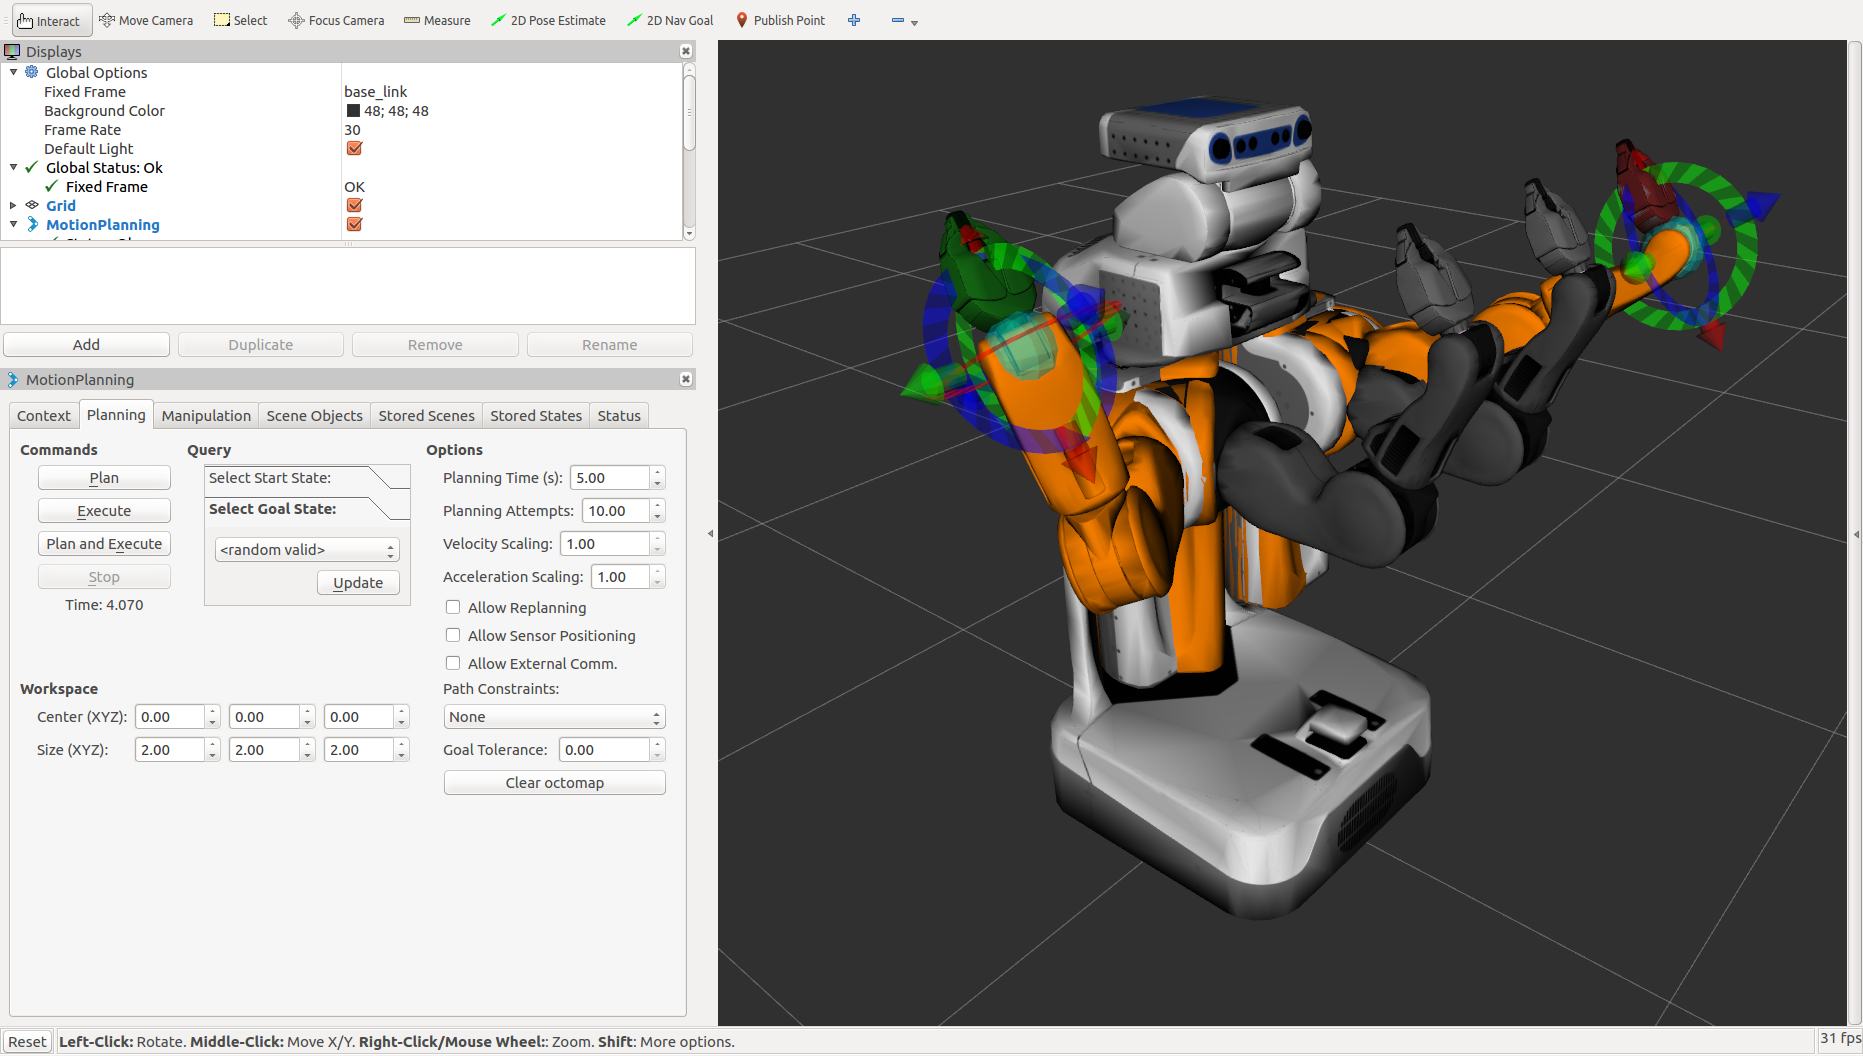
\includegraphics[width=\textwidth]{images/moveit_rviz.png}
    \caption{Screenshot captured by the author of an RViz instance using MoveIt! to plan on a PR2. The orange limbs are the desired state.}
    \label{fig:moveItExample}
\end{figure}

\subsubsection{OpenRAVE}
Open Robotics Automation Virtual Environment (OpenRAVE) is a research-grade software environment which includes methods of modeling different robots and environment objects through a simulation engine to serve as a platform for experimenting with and validating motion planning algorithms. \cite{openRave} OpenRAVE also includes the IKFast module, which can generate very quick C++ code that analytically solves the IK for robotic manipulators described in the OpenRAVE-supported robot description format. \cite{ikFast} C++ and Python API's are available for interacting with OpenRAVE, and it can be installed on Ubuntu and Windows with Visual Studio. There is decidedly a smaller community supporting OpenRAVE than its ROS counterpart, MoveIt!, but OpenRAVE can be used in ROS installations with some additional setup to allow access to IKFast and other tools. \autoref{fig:openRAVEExample} shows a screenshot of an OpenRAVE environment being used for planning on a PR2 humanoid.

\begin{figure}[thpb]
	\centering
	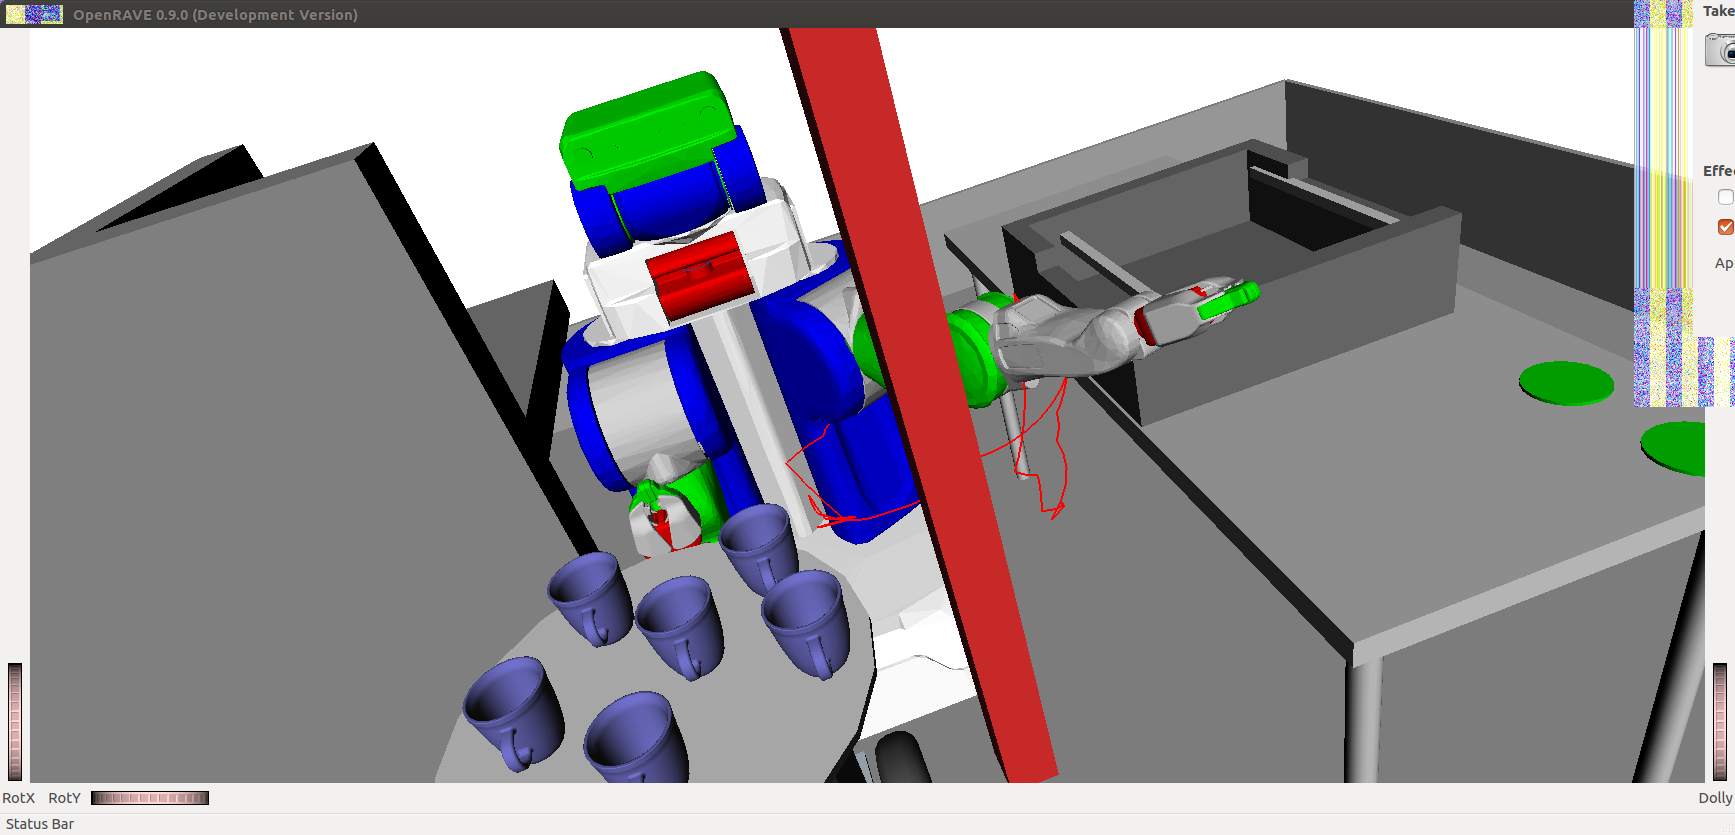
\includegraphics[width=\textwidth]{images/openrave_pr2_planning.png}
    \caption{Screenshot captured by the author of an OpenRAVE instance with a PR2 in a simulated environment completing a motion planning problem.}
    \label{fig:openRAVEExample}
\end{figure}


%%%%%%%%%%%%%%%%%%%%%%%%%%%%%%%%%%%%%%%%%%%%%%%%%%%%%%%%%%%%%%%%%%%%%%%%%%%%%%%%
\chapter{System Design}
This chapter is concerned with the first step of this project: defining the objectives and requirements of the system, deciding how to integrate the system in surgical procedures, and designing the software infrastructure to support the functions that need to be fulfilled. The system is designed to be generic and adaptable to different procedures, but focuses on specific implementation on the neurobot.


\section{System Objectives}
\label{sec:systemObjectives}
% this is where we list use cases, features, etc.
This project has the following objectives to accomplish in order to successfully fulfill the user need:

\begin{itemize}
\singlespacing
\item Interfaces with existing medical platforms including the robot control system and 3D Slicer.
\item Accurately assesses robot workspace considering the environment and entry point into the body.
\item Generates collision-free trajectories from the robot's starting configuration to the entry point in the body.
\item Segments the patient into a 3D volume for collision avoidance.
\item Provides a mechanism for assisting surgeons with selecting an optimal insertion point in the body to most readily reach the treatment location.
\end{itemize}

\section{System Requirements}
There are some additional considerations that can impact how the system can be designed. These have been organized into the below list of requirements the system must abide by.

The system shall...
\begin{itemize}
\singlespacing
\item Operate on Windows, Mac, or Linux computers.
\item Be easy to install and use by a non-technical user.
\item Be packaged for portability and distribution.
\item Be readily accessible to new developers in the lab.
\item Communicate with the robot using OpenIGTLink.
\item Utilize 3D Slicer as the user interaction interface.
\item Communicate with 3D Slicer using OpenIGTLink.
\end{itemize}


\section{Surgical Workflow}
\label{sec:surgicalWorkflow}
During procedures with the neurobot, there is an established workflow as discussed in \autoref{sec:neuroablationProcedures}. The software system being developed in this project will redefine that workflow, and it is important to consider how the system can best modify that workflow to effectively make use of its new features. \autoref{fig:surgicalWorkflowPg1} and \autoref{fig:surgicalWorkflowPg2} functionally illustrate the workflow during a procedure making use of this system. A high-level overview of the workflow is as follows:

\begin{enumerate}
\item Register the robot in the scanner and send offsets for planning.
\item Send the patient head as a model to the software system.
\item Software system sends a workspace of reachable entry points to 3D Slicer.
\item Surgeon selects entry point. System computes the ultrasonic element workspace given that entry.
\item Target point is selected. System computes motion plan from current configuration to entry.
\item Operator examines plan and sends to robot controller.
\item Robot executes motion. Cannula and probe are attached to robot. 
\item Robot inserts probe and ablation(s) are performed. 
\item Cannula and probe are removed from patient. Robot is removed from scanner.
\end{enumerate}

In some cases, not all of the steps above would be performed during procedures. A procedure could start at Step 4, assuming the robot registration had already been performed, and skip the entry workspace check if the operators were familiarized with the reachable entry workspace of the robot. In future iterations of the design, the entry point could also be automatically selected based on MR image analysis to locate the burr hole.

\begin{figure}[thpb]
	\centering
	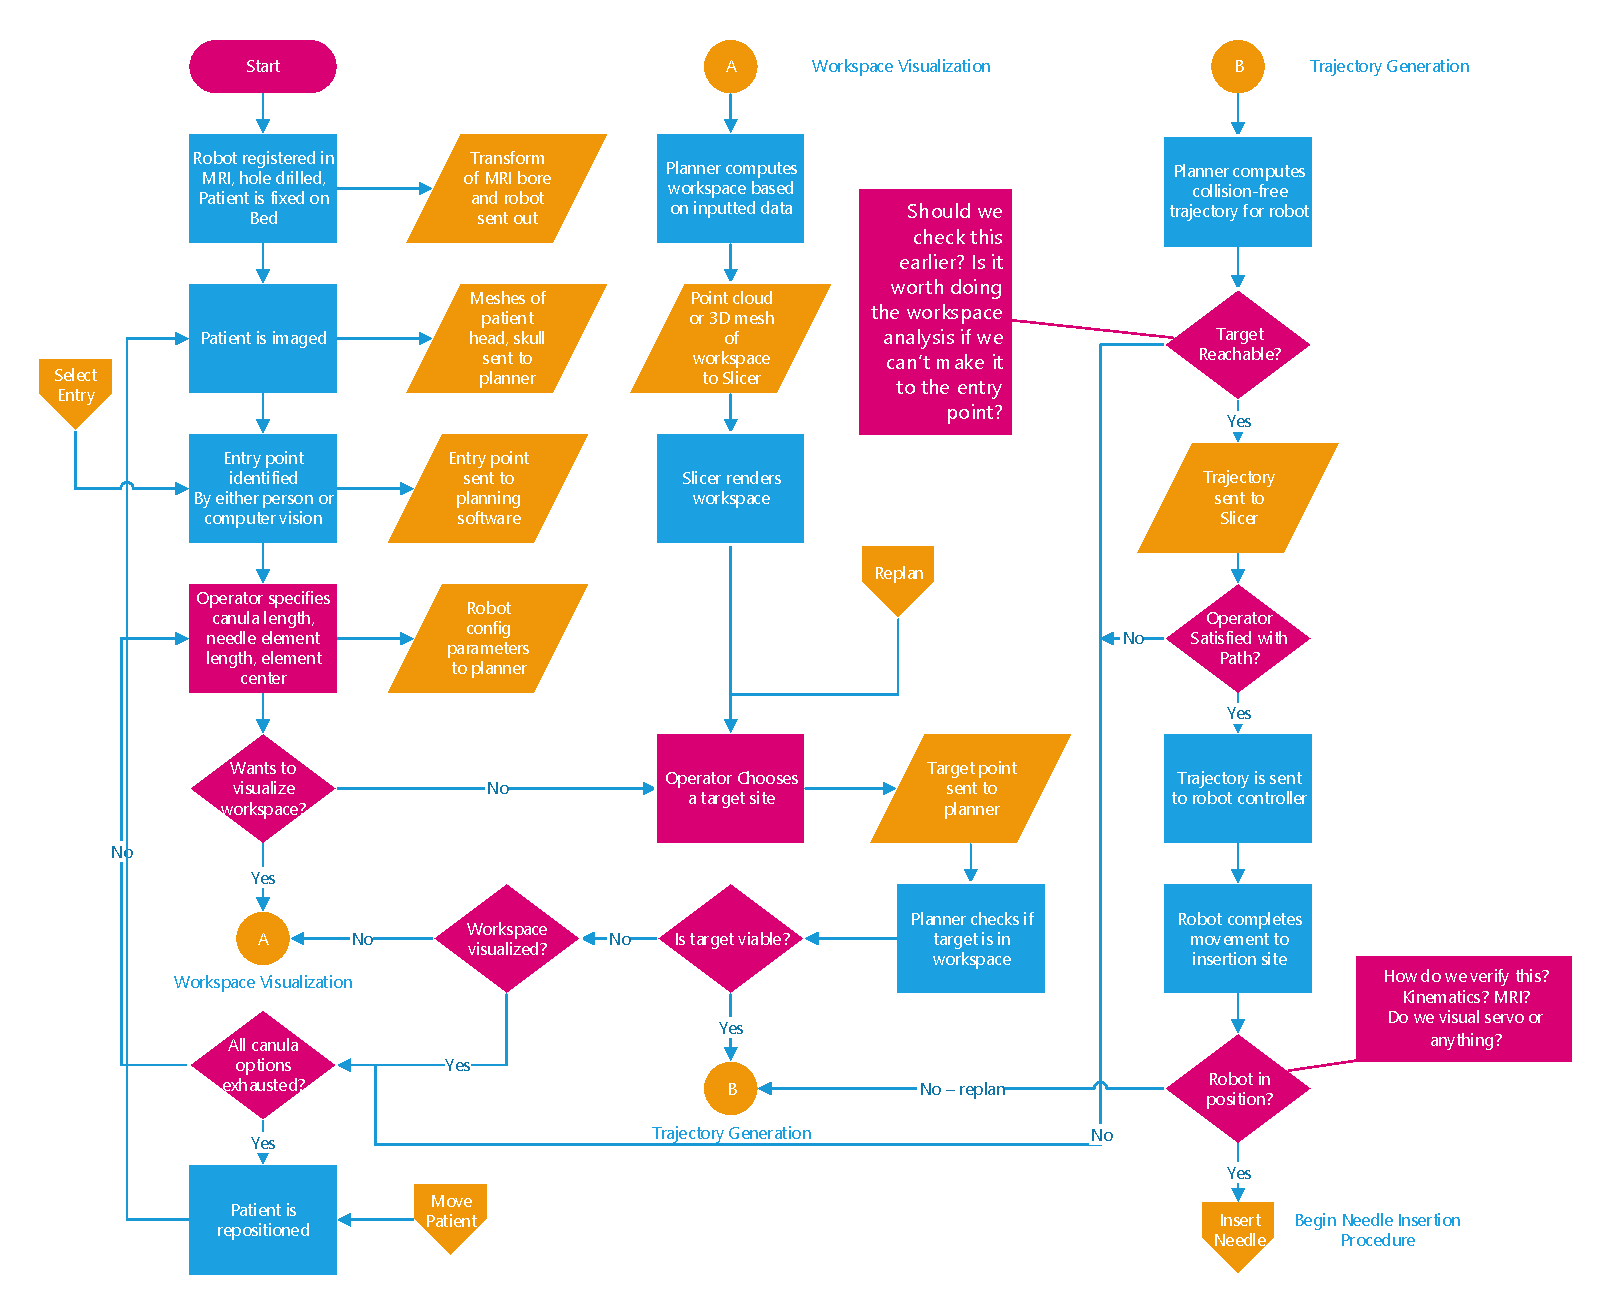
\includegraphics[page=1,width=5in]{diagrams/Surgical_Workflow_-_Hole_Predrilled.pdf}
    \todo[inline]{Update workflow diagram. GF: make these as big as you can fit on the page}
    \caption{Diagram of the surgical system workflow when the hole is drilled before the patient is placed on the MRI bed. Page 1 showing procedure setup, worskspace visualization, and trajectory generation.}
    \label{fig:surgicalWorkflowPg1}
\end{figure}

\begin{figure}[thpb]
	\centering
    \includegraphics[page=2,width=5in]{diagrams/Surgical_Workflow_-_Hole_Predrilled.pdf}
    \caption{Diagram of the surgical system workflow when the hole is drilled before the patient is placed on the MRI bed. Page 2 showing needle insertion procedure and extraction.}
    \label{fig:surgicalWorkflowPg2}
\end{figure}


\section{Software Design}
Based on the objectives and requirements for the system at consideration, the following approach has been formulated. The motion planning is completed using MoveIt!, utilizing ROS as the system for managing the robot configuration and model. This choice is driven by the capability of OMPL, the streamlined collision checking with the environment in MoveIt!, strong community support and knowledge of ROS and MoveIt!, and the ease of installing and maintaining the ROS software environment. Initially, development began with the hope of installing OMPL on a Windows machine since this operating system was most commonly used in the hospital and this could allow OMPL to be used directly from within a Slicer module built in C++. Unfortunately, source installation of OMPL was necessary, unsupported by the OMPL developers, and several other dependencies for running OMPL were equally as challenging to install. After some time was spent trying to overcome these barriers (some resources and instructions for the progress made on this endeavor can be found in \autoref{sec:omplWindowsInstallation}), it was decided that even if a solution could be found, the complexity of the install process was too great and increased the risk of the software failing to be easy to install and configure on new systems. Thus it was decided that having a separate computer (or virtual machine) running Ubuntu was acceptable given the ease of setting up OMPL through ROS on that platform. 

ROS and MoveIt! are installable on Ubuntu by a single scripted command and officially supported on Long Term Support (LTS) Ubuntu releases, increasing the potential lifespan of the software system before needing upgrades. This is further discussed in \autoref{developmentConfiguration}. The motion planning code would then run on an Ubuntu computer linked to the robot and Slicer over OpenIGTLink. Alternatively, a Virtual Machine (VM) running Ubuntu can be hosted on a Windows machine to reduce the number of computers needed to run the neurobot during procedures.

\autoref{fig:softwareDiagram} shows the software modules and data interfaces between the ROS packages for workspace analysis and motion planning, the Slicer module for interacting with the workspace data, and the robot controller. A key component for managing the interface between ROS and Slicer is the ROS-OpenIGTLink-Bridge package, which connects to OpenIGTLink interfaces and exposes that data on the ROS network via custom messages, as discussed in \autoref{sec:rosOpenIgtlinkBridge} This allows a clear separation between OpenIGTLink-connected software and ROS connected software.

\begin{figure}[thpb]
	\centering
	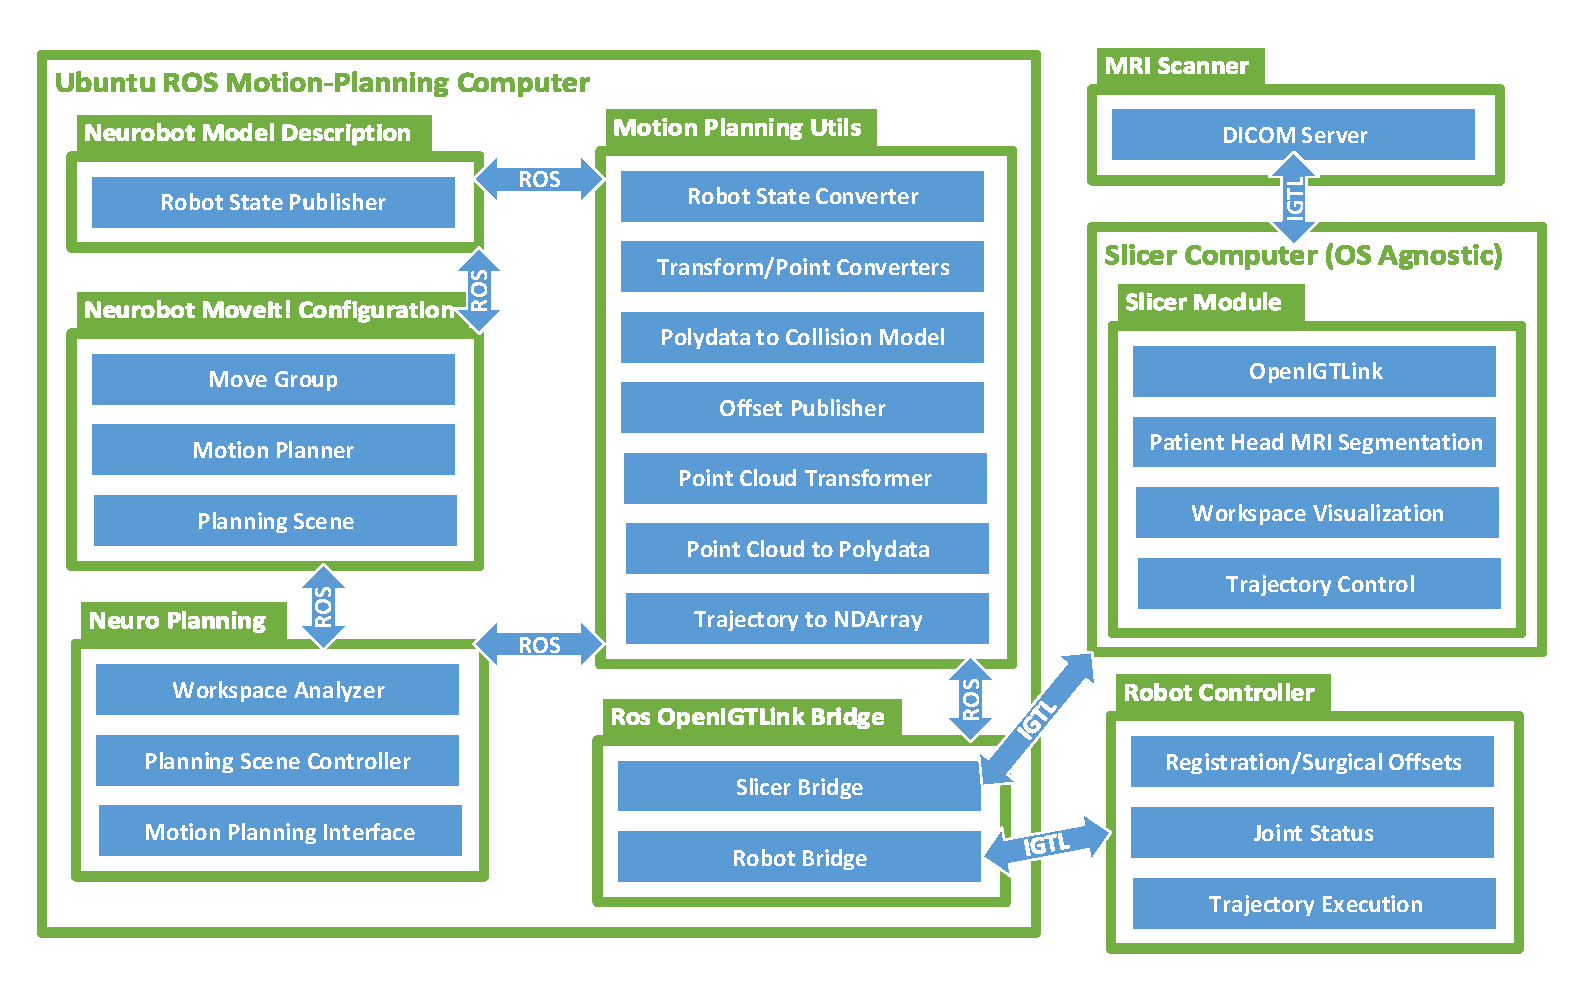
\includegraphics[width=\textwidth]{diagrams/Software_Diagrams_Simplified.pdf}
    \caption{Diagram of the software architecture showing interfaces between ROS packages and 3D Slicer. The groupings in the green boxes on the ROS computer represent ROS packages where each blue box is a node; for the systems on the right, these represent different functions. }
    \label{fig:softwareDiagram}
\end{figure}


%%%%%%%%%%%%%%%%%%%%%%%%%%%%%%%%%%%%%%%%%%%%%%%%%%%%%%%%%%%%%%%%%%%%%%%%%%%%%%%%
\chapter{System Implementation}
This chapter covers the development setup of the system, implementation of key interfaces, and the packaging of the software for use in the field.


\section{Development Configuration}
\label{developmentConfiguration}
The system was designed to run on a Ubuntu 16.04 computer with ROS Kinetic installed. Typically, ROS releases are tied to specific Ubuntu releases, and LTS versions are supported with security patches and bug fixes for five years after release with new releases every two years. Usually, ROS versions are generally API-compatible between sequential versions, but changes to the API structure may throw warnings during compilation that those API functions are being changed or removed in the next ROS version. Over a greater time period, ROS 1 will generally remain consistent across yearly revisions, but ROS 2.0 is not expected to maintain API compatibility. Installing 3D Slicer on this system was optional and trivial, but at least one computer had to have Slicer installed for conducting the procedure. The most recent stable Slicer program  was used, which was 4.8.1. Beyond the simple one-line installation of ROS and MoveIt!, OpenIGTLink had to be downloaded and built from source using a script. With those simple dependencies installed, software was ready to be built.

\subsection{ROS Workspace}
A standard catkin build tools workspace was created for building and sourcing the ROS packages for the software platform. A git repository contained the code for the project and could be cloned and built in the catkin workspace alongside other ROS packages. Nodes were written in C++, and \autoref{fig:rosNodeGraph} shows the network of running ROS nodes the topics used for message transport.

\begin{figure}[thpb]
	\centering
	
\includegraphics[width=\textwidth]{diagrams/rosgraph_workspace_clipped.pdf}
    \todo[inline]{Needs to be readable when printed}
    \caption{Graph of ROS nodes and topics on the completed system. }
    \label{fig:rosNodeGraph}
\end{figure}


\section{Bridging with OpenIGTLink}
The ROS-OpenIGTLink-Bridge package simplified the task of interfacing with OpenIGTLink, yet it did not complete all of work that was necessary to complete the integration of the two systems. The ROS-OpenIGTLink-Bridge defined its own messages, so packages needing to subscribe to topics using those message types had to specifically include the bridge package to build. This ran contrary to the goal of having the ROS-based workspace analysis and motion planning be agnostic to OpenIGTLink and able to operate entirely within the ROS environment. Consequently, nodes were written which were parameterized to allow conversions from the OpenIGTLink messages to standard ROS messages, and the following sections document some of the key interfaces of the system. Additionally, these nodes also performed unit conversion from ROS (using meters) to Slicer (using millimeters). Potentially, it would be useful to push these conversion nodes to the bridge project as this would allow for better compatibility with ROS systems which already exist and do not need to be rewritten to use the bridge data types.

An advantage of the ROS communication paradigm was that two OpenIGTLink connections could be made, one to Slicer and one to the robot, yet both would be exposed to the same topics on ROS. In other words, the ROS system did not care (and could not tell) how many different OpenIGTLink connections provided and sent the information to them. This provided additional flexibility in allowing the target and entry points to be defined by the robot control software as well as from an operator using Slicer.

\subsection{Transferring Frames}
The key transform necessary for the software system was the registration transform from the optical frame of the scanner to the z-frame (also the base frame) of the robot. This transform was sent through OpenIGTLink by the robot control software, and a node was written to take the IGTLink transform published by the ROS-openIGTLink-bridge package and publish it as a transform to the TF2 package. This transform would then be used to transform incoming entry and target points into the robot's frame of reference for the purposes of workspace analysis and motion planning. \autoref{fig:rosTFTree} shows the TF tree in ROS.

\begin{figure}[thpb]
	\centering
	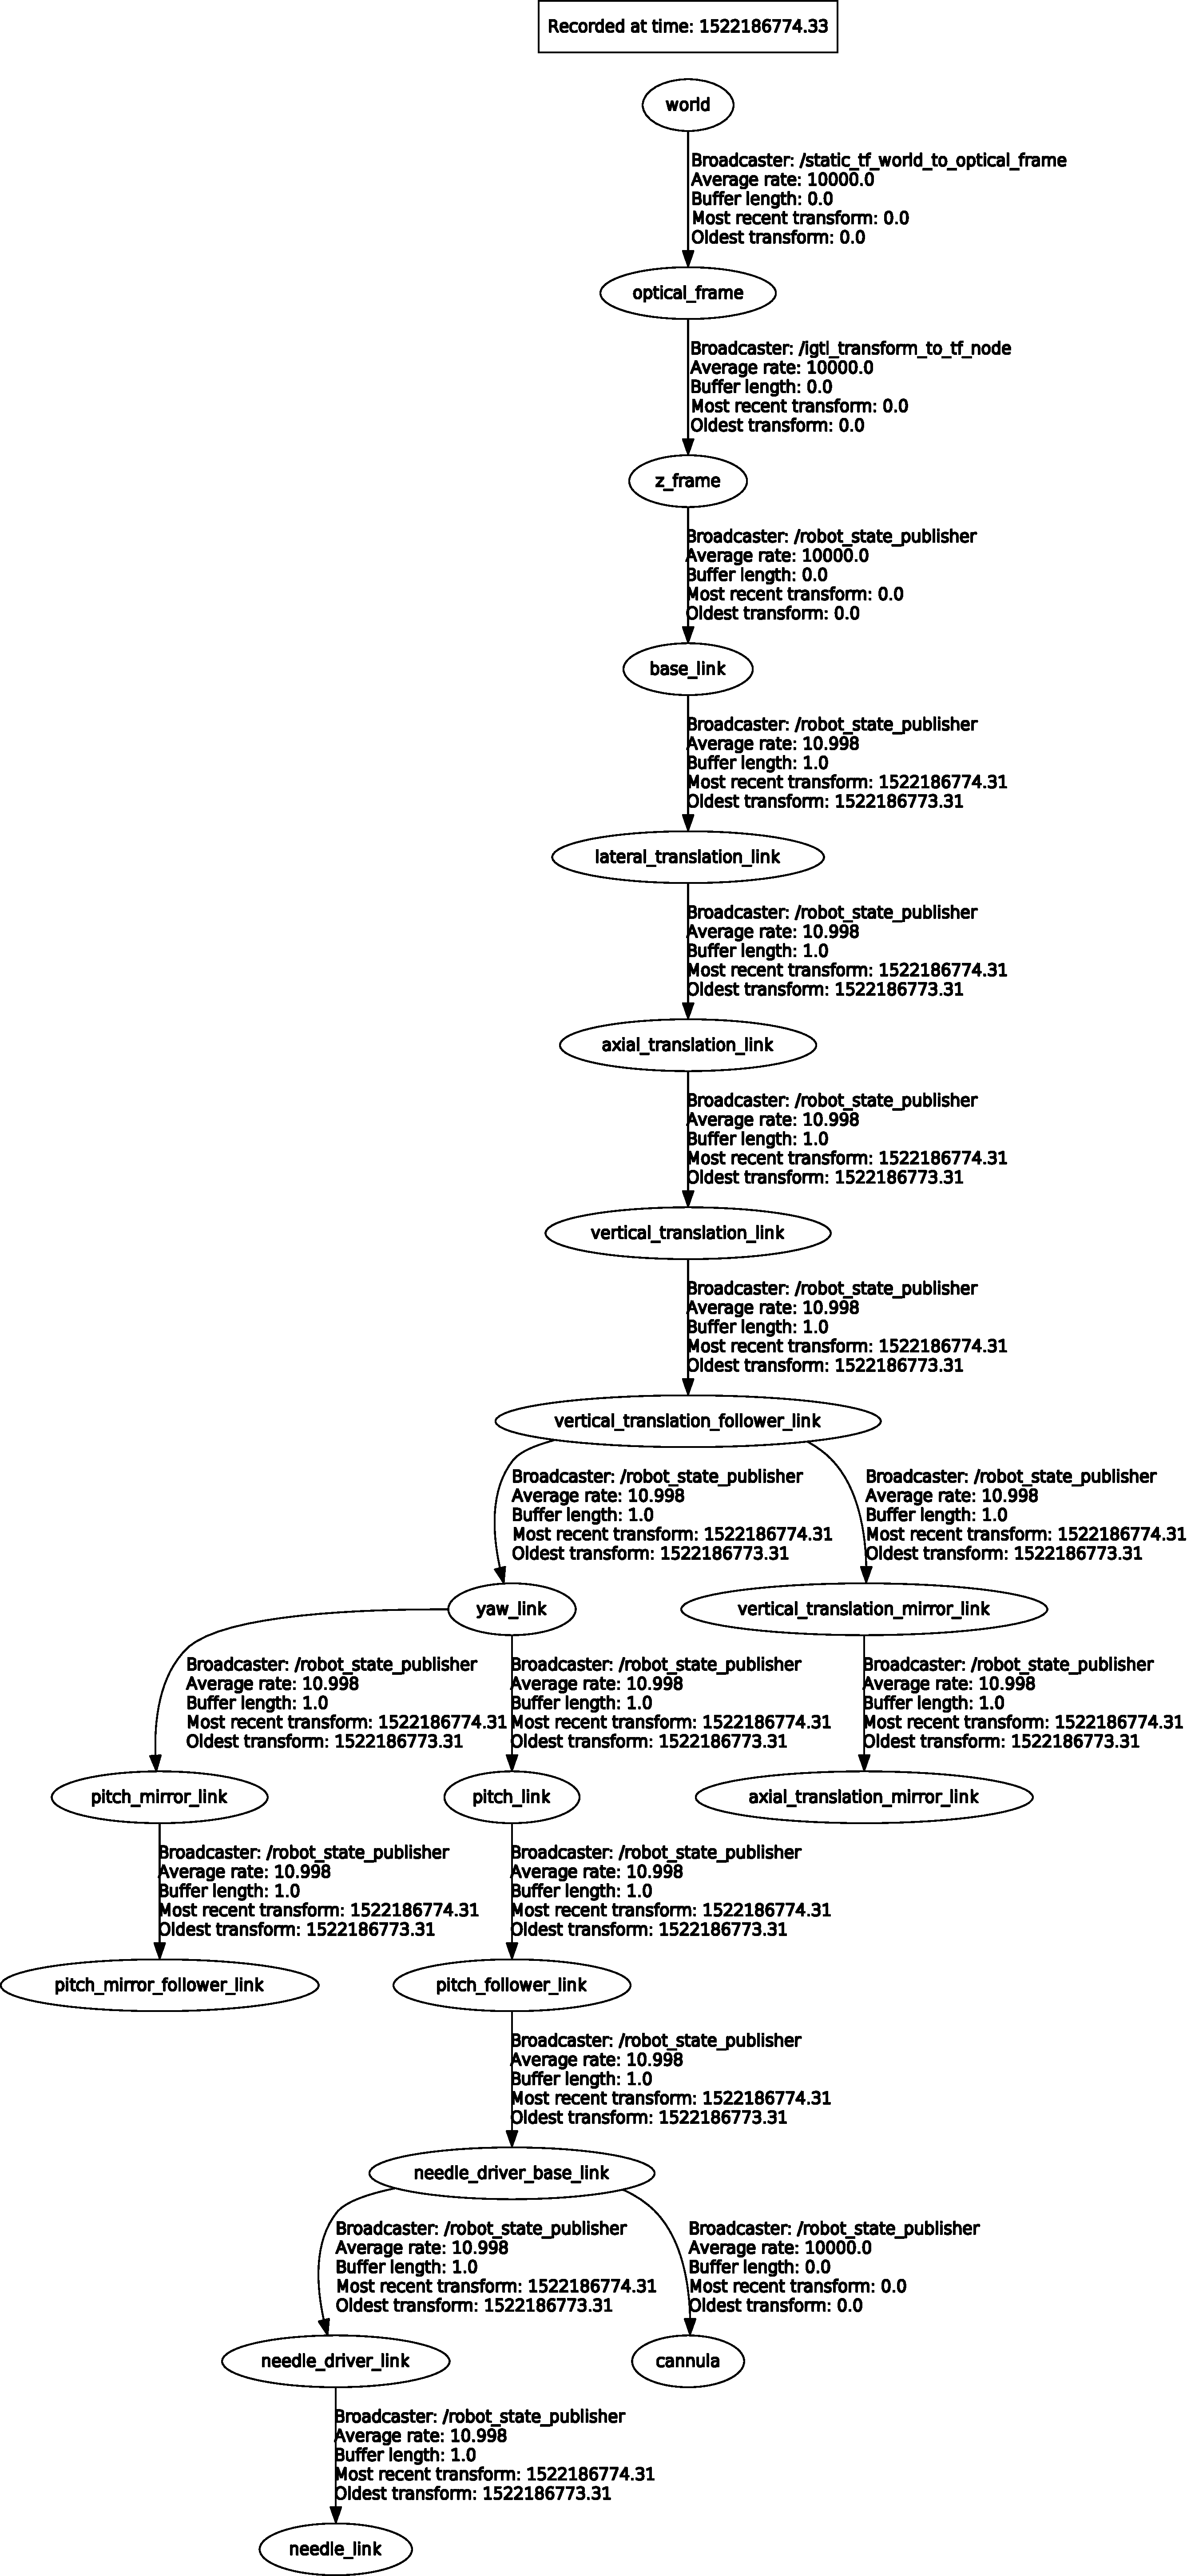
\includegraphics[height=6in]{diagrams/neuro_tf_frames_clipped.pdf}
    \caption{TF tree of the system showing the transforms defined in ROS. }
    \label{fig:rosTFTree}
\end{figure}

\subsection{Transferring Offsets and Points}
Additional nodes were written to convert the IGTLink points into geometry point stamped messages so that those points could be transformed into the coordinate frame in which subscribing nodes would be doing processing. Unfortunately, points sent over OpenIGTLink did not have transform data associated with them. In other words, all points (as is the case with Slicer) are specified in the optical scanner frame. This necessitated writing the nodes such that this assumption could be changed or specified as needed.

The offsets discussed in \autoref{sec:neuroablationProcedures} were transferred as OpenIGTLink string types since the bridge did not include the OpenIGTLink double or float types. Nodes then converted these strings into messages that were simply published as floats. Alternatively, and better following ROS practices, these offsets could be updated with a dynamic reconfigure server instead of being published on separate topics.

\subsection{Sending Workspace Volume}
\label{sec:sendingWorkspaceVolume}
% originally marching cubes, then concave hull
The workspace was generated as a point cloud by the workspace analysis ROS package, so a node had to convert the point cloud into a format for OpenIGTLink. While there was a type for fiducial points, publishing over around 700 points caused Slicer to hang and run very slowly once all the points were loaded. Thus a different format was needed.

When viewing the MRI scan planes, Slicer overlays polydata meshes on whatever slice was being viewed. This was ideal for visualizing the workspace as it pertained to the procedure planning. Polydata could contain points, polygons, vertices, strips, and lines. Seeing only points representing the workspace reduced the understanding of the workspace boundary, and the points were also very difficult to see in Slicer due to the size in which they were rendered. However, meshes (consisting of polygons) were very easy to see from different slice perspectives and allowed a more intuitive interpretation for what was reachable within the boundary of the mesh.

A node was written which converted the point clouds to polydata meshes using the Point Cloud Library (PCL) and VTK data conversion tools. The ROS point cloud was converted to a PCL point cloud which allowed the point cloud to be processed using PCL's built-in manipulation tools. Under the recommendation of a developer of the ROS-OpenIGTLink-Bridge, the marching cubes reconstruction algorithm was first implemented, but this attempted to create a mesh which best connected the surface normals of all the points, whether they were points on the edge of the workspace or if they were points within the workspace, which resulted in some broken borders and internal meshes in the workspace. Once this was attempted, a concave hull approximation was used instead, which essentially tries to shrinkwrap a mesh around a point cloud. This achieved the desired result, and after some parameter tuning to ensure a smooth shape which closely held to the underlying structure of the point cloud, point clouds in ROS could be sent over OpenIGTLink to Slicer as seen in \autoref{fig:cubeMeshConversion}. 

\begin{figure}[thpb]
	\centering
	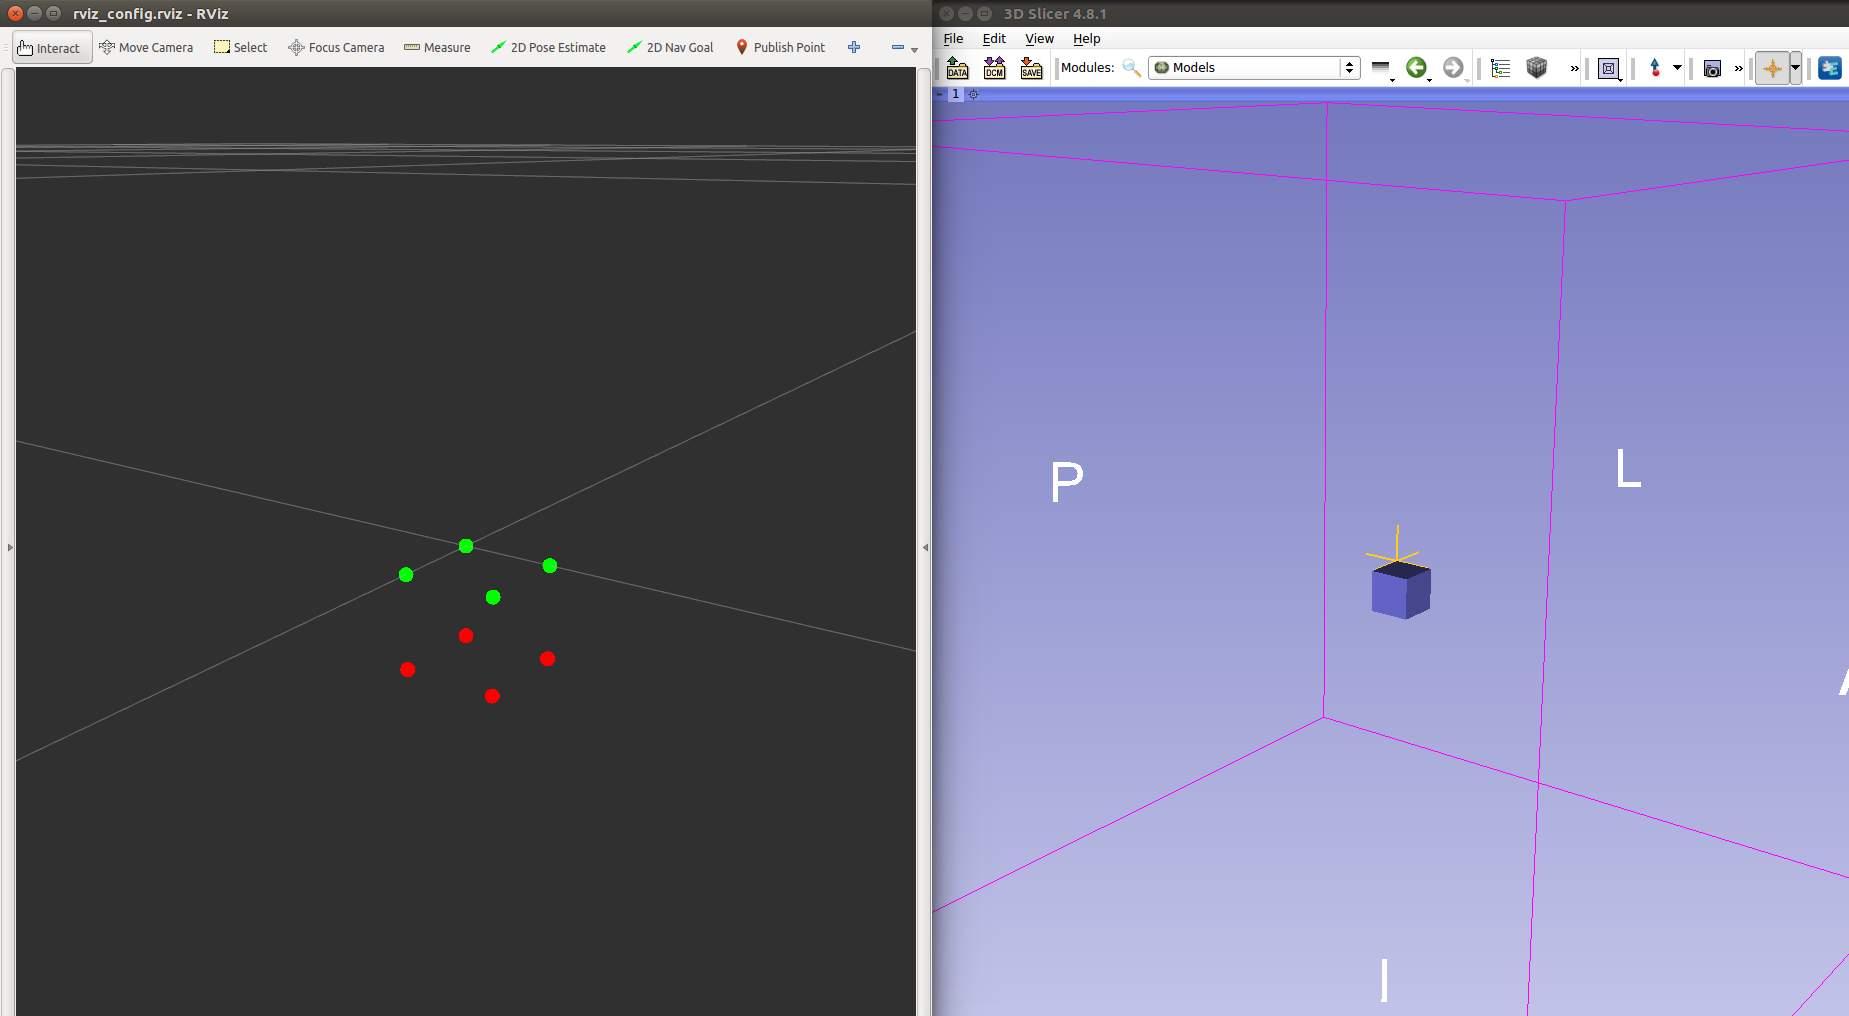
\includegraphics[width=\textwidth]{images/cube_mesh_rviz_slicer.png}
    \caption{A point cloud of a cube in ROS (left) with the resultant polydata mesh object in Slicer (right).}
    \label{fig:cubeMeshConversion}
\end{figure}

In slicer, the 3D displays under the model module had to be changed to show all surfaces, not just what Slicer thought was the front planes. When this viewing option was not selected, the mesh would appear jagged and incomplete, as seen in \autoref{fig:cubeMeshConversionBadView}. This was simply an issue with the way Slicer attempted to show through parts of the mesh, but toggling the option for that model to show the full surface rendered it properly as seen in \autoref{fig:cubeMeshConversion}.

\begin{figure}[thpb]
	\centering
	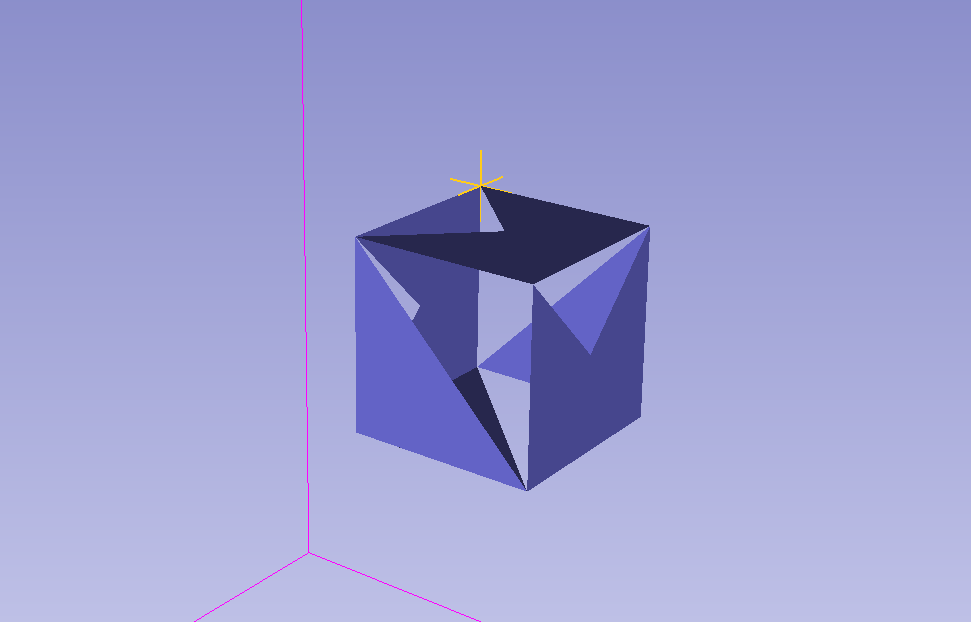
\includegraphics[width=4in]{images/jagged_slicer_mesh.png}
    \caption{Polymesh object in Slicer with only the front faces being rendered, resulting in a choppy-looking mesh.}
    \label{fig:cubeMeshConversionBadView}
\end{figure}

\subsection{Receiving Robot State}
\label{sec:receivingRobotState}
For the purposes of motion planning, the robot's starting configuration needed to be known. With the robot modeled in ROS, the joint state publisher would hold the state of the robot, but as will be discussed in \autoref{sec:transformJointSpace}, a difference between the ROS model and the actual robot necessitated a conversion between the two joint spaces, which was done using ROS message types. With this transformation in place, the joint state had yet to be communicated between OpenIGTLink and ROS, and this proved to be somewhat of a challenge. The ND Array type in OpenIGTLink was ideal for holding this information, but this was not implemented in the ROS-OpenIGTLink-Bridge package. The bridge package repository was forked and the ND Array type was attempted to be added as a message and to the bridge. Unfortunately, the implementation of this was difficult on both the ROS side and the robot controller due to lack of documentation and samples utilizing the ndarray data standard. Instead, the joint state was sent as a string of comma separated values. Then a node was written that took properly named incoming strings representing the robot's state sent from the robot controller and published those as a ROS joint state message, which could then be transformed into the modeled state and sent to the robot joint state publisher so that the motion planning package and other packages using the TF library could use the updated robot state.


\subsection{Sending Joint Trajectories}
Trajectories in ROS were well standardized as messages with a list of joint names and a list of joint trajectory points which included position, velocity, accelerations, and effort of each of the active DOF and a duration time from the start of the trajectory at which that trajectory point was to be achieved. Of course, this format did not exist in OpenIGTLink, so another conversion had to be made. Again, the NDArray type would have been most suitable, but instead a string was used, in which a time stamp, joint positions, and joint velocities were sent separated by semicolons and commas. For instance, the joint positions were listed with commas while a semicolon separated both the duration time and the joint velocities. A node listened to trajectories being published from the motion planner, transformed the joint space as discussed in \autoref{sec:transformJointSpace}, converted units, and sent those messages over OpenIGTLink. The robot controller would then parse this array to perform the desired trajectory.

To provide a method for visualizing the trajectory in Slicer before approving it and allowing the controller to perform the action, another array was sent which contained the end effector position as an array at each state in the trajectory. This removed the need to have a FK solver bundled within Slicer. \todo{Revisit this when completed.}


\section{Software Packaging}
In order for the system to run on Windows and Mac systems, a VM image of Ubuntu 16.04 was created and maintained with ROS, MoveIt!, and OpenIGTLink installed. Oracle's VirtualBox was the virtual machine monitor used, but others were compatible with the VM image format as well. The image was essentially identical to the setup on a developer computer, but included scripts on the desktop for downloading and rebuilding code changes for the software, automatic login, and shortcuts for configuring OpenIGTLink parameters to adjust changes in the robot's or Slicer's IP address. The VM was run on the laptop computer which ran the Slicer interface during procedures, where the entry and target points would be specified while viewing the MRI captured of the patient.


\section{Software Documentation}
As with all software projects, documentation of code is key for enabling the system to continue to be useful and ensure that changes can be made easily. Documentation from a non-technical user perspective is written so that new operators can learn how to use the system without necessarily being trained personally. The user documentation can be found in \autoref{sec:userDocumentation}. Code is commented throughout, but having dedicated technical documents for specific procedures to complete routine changes to the software is necessary. \autoref{sec:technicalDocumentation} contains the technical writings developed during the course of this project.


%%%%%%%%%%%%%%%%%%%%%%%%%%%%%%%%%%%%%%%%%%%%%%%%%%%%%%%%%%%%%%%%%%%%%%%%%%%%%%%%
\chapter{Neurobot ROS Modeling}
In order to utilize the tools within ROS for completing collision detection and conducting motion planning with MoveIt!, the robot had to be modeled in a ROS-compatible format, as discussed in \autoref{sec:ros}. This chapter discusses modeling the neurobot in ROS, creating its MoveIt! package, modeling environment objects, and interacting with the system and visualizing its outcomes.


\section{Representation of Neurobot Kinematics}
Generating this particular robot model in ROS required a bit more processing than a normal serial manipulator. The URDF does not allow closed loop linkages since the kinematic structure of the robot is eventually described using TF, which expresses coordinate frames as a tree structure. This complicated the development of an accurate model since the neurobot includes parallel linkages in the design, resulting in more joints than degrees of freedom. Further, as described in \autoref{sec:kinematicsJointInfo}, axial and vertical motion is attained through a pair of lead screws, where the differential between the two achieves vertical motion and synchronized actuation produces axial motion. 

A workaround the limitation of the URDF to describe closed loop chains was to use mimic tags, \todo{GF: maybe a figure point out where you used this} which describe how one joint mimics or follows the pattern of another and removes the mimicing joint from the list of the robot's active DOF. This allowed the parallelogram linkage mechanism, which was actually two prismatic joints, to be modeled as two decoupled joints with a prismatic joint for axial translation and a revolute joint for changes in height. Two separate chains with a single active degree of freedom that controlled the height through rotations on one linkage. A similar mimicing pattern was used for the pitch axis, and the result of the final modeling of the neurobot is shown in \autoref{fig:neuroROSModel}.

\begin{figure}[thpb]
	\centering
	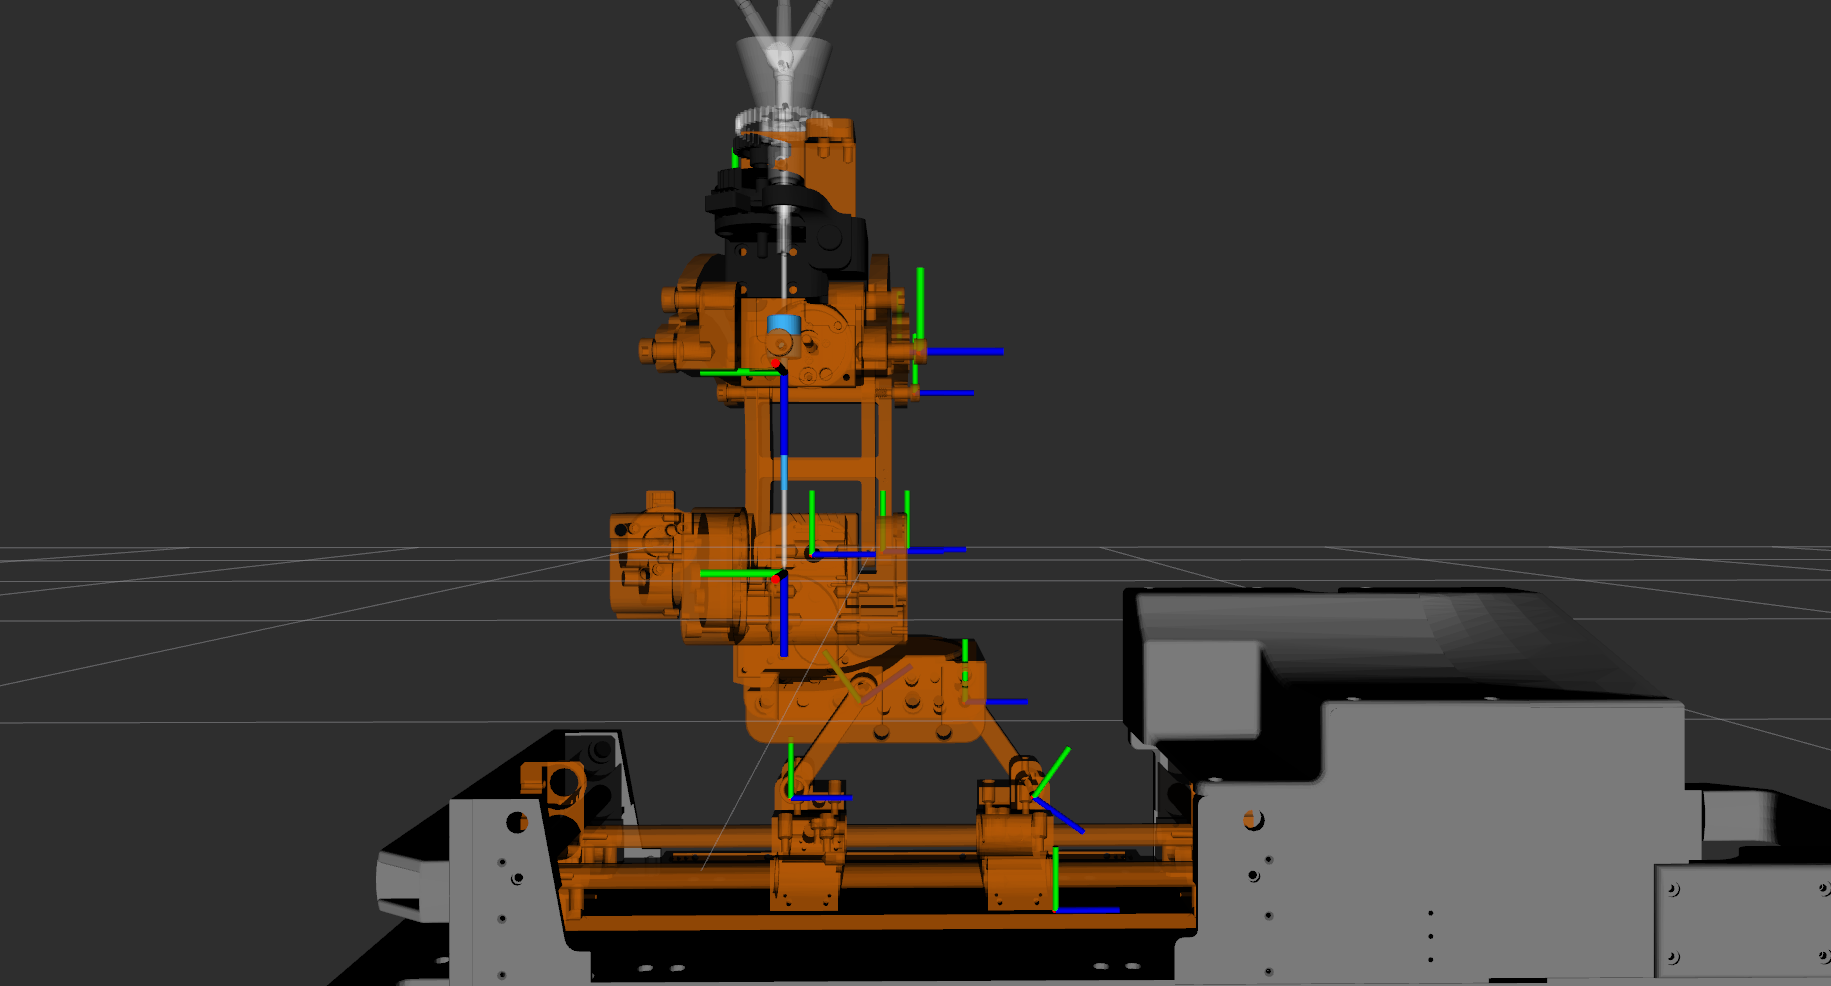
\includegraphics[width=\textwidth]{images/rviz_screenshot_2018_model.png}
    \caption{The finished ROS model of the neurobot showing joint frames on the parallelogram structure. Height was changed by rotating the bottom right joint on the linkage.}
    \label{fig:neuroROSModel}
\end{figure}

\subsection{Exporting Robot Model to ROS}
The robot was drafted in SolidWorks as an assembly of several parts and subassemblies. Fortunately, a tool (creatively) named ``Solidworks to URDF Exporter'' was available as a SolidWorks add-in that simplified the creation of URDF's by starting from a SolidWorks assembly. \cite{urdfExporter} General operation included opening up the add-in window and selecting parts or assemblies that represented a linkage on the robot, defining the frame and axis for each joint, selecting the joint type, and building a tree structure of joints which could be converted into a URDF format by exporting the URDF and properly generating STL files of the robot geometry. A screenshot of the tool in action can be seen in \autoref{fig:solidWorksExport}.

\begin{figure}[thpb]
	\centering
	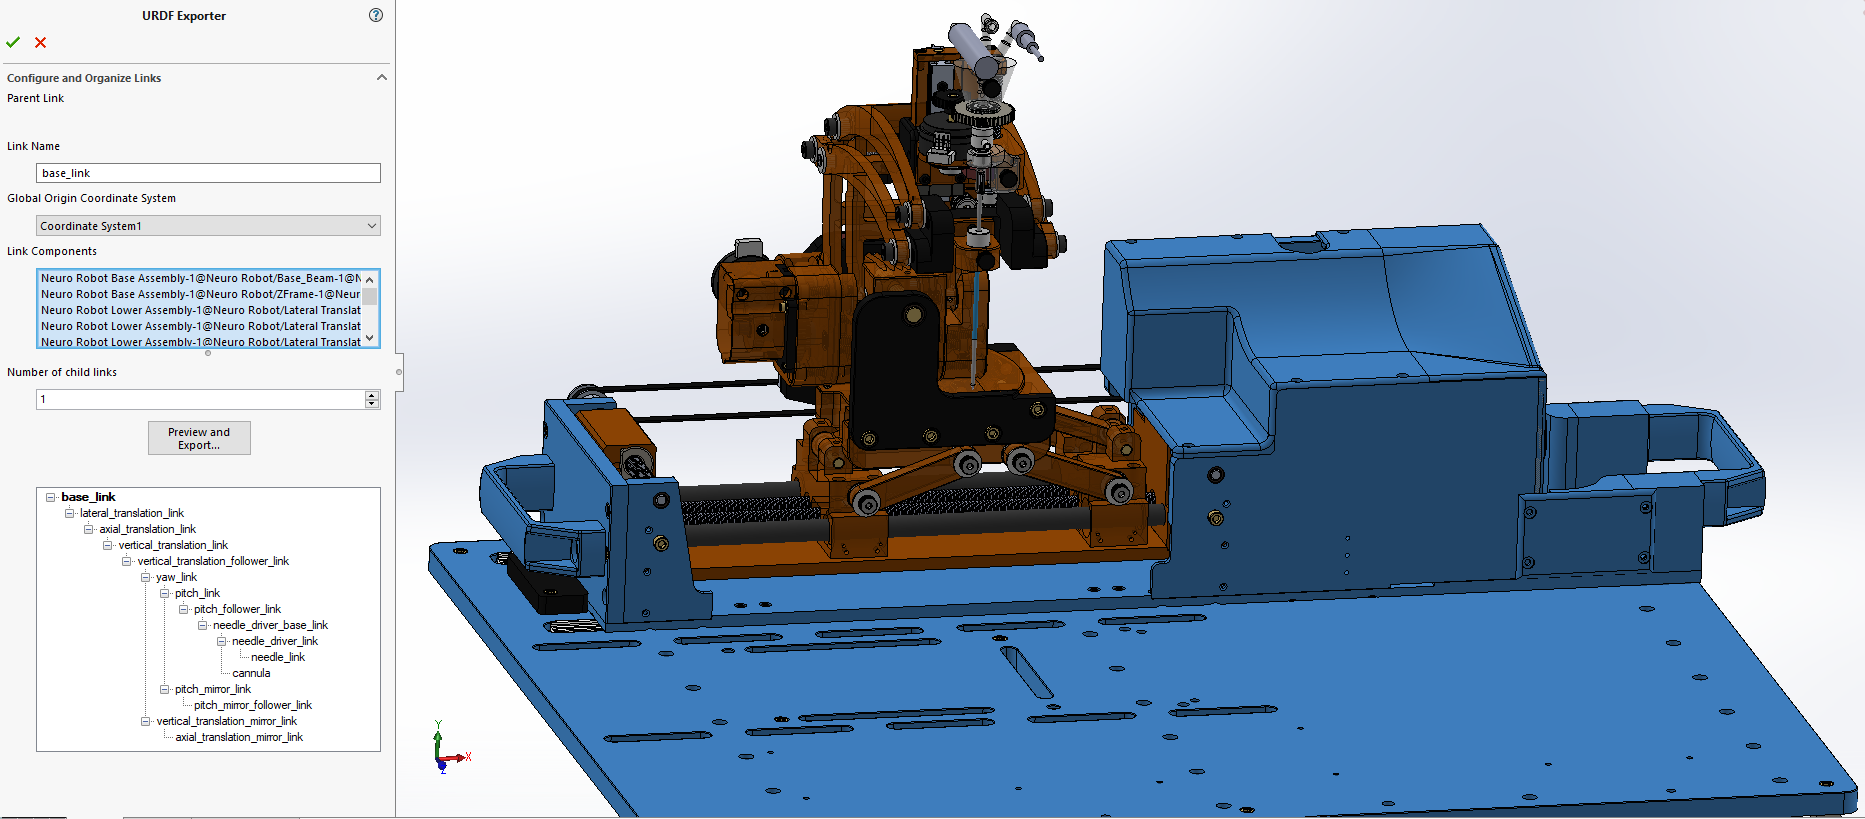
\includegraphics[width=\textwidth]{images/solidworks_to_urdf_screenshot.PNG}
    \caption{Screenshot of the SolidWorks to URDF add-in being used on the neurobot assembly. The left panel shows the kinematic tree and joint options for the base link.}
    \label{fig:solidWorksExport}
\end{figure}

While the add-in featured an auto-detection tool for identifying joint types, this did not work for the neurobot, and presumably would only work on simple serial mechanisms that were properly constrained to move only at the joints. Rather, at every joint, a coordinate frame had to be created which defined the zero location of the joint, and an axis was also defined through that coordinate frame around which (or along which) movement on that joint would be rendered. Of somewhat inconvenience, these frames and axis had to be created in the top-level assembly; when these were defined in subassemblies, the export process would improperly assign frames and the STL files were not properly transformed to the right frames.

Once the joints were assigned and defined in the tree structure with the associated parts assigned to each linkage, the export process could begin. Joint limits, movement axis directions, efforts, and velocities were specified for each joint, rotational inertia and mass properties were inputted, colors were specified for linkages, and the ROS package was generated. However, some of these parameters, such as the joint limits, were not saved in the configuration file and had to be regenerated every time the URDF was exported. Once generated, the package was placed directly in the repository for the software system, but the following fixes had to be made:
\begin{itemize}
\item The package author needed to be specified to allow the package to build in current versions of ROS.
\item Paths in launch files had to be corrected to point at the URDF in the proper folder.
\end{itemize}

\subsection{Final URDF Cleanup}
Some further tweaks were necessary to the URDF once it was generated by the SolidWorks to URDF add-in, which are further documented in \autoref{sec:userDocumentation}. Since some of the parameters for generating the URDF had to be reentered every time the package was generated, sometimes it was easier to edit the joint limit information after the fact. There was some trial and error involved with correcting motion directions, usually amounting to a sign flip to have the joint values increment and decrement as desired. Velocities also had to be specified for the joints so that generated trajectories would not try to move the joints in each time step faster than they were capable of moving. Once the joint limits, velocities, and directions were corrected, mimic tags were added to joints appropriately to achieve the desired kinematic chain. In the end, the robot had seven active degrees of freedom with seven additional joints that were either fixed or mimicing the active joints to produce the correct motion of neurobot, and the GUI for controlling the simulated robot is shown in \autoref{fig:jointStatePublisherGUI} with a rendering of the neurobot with the base plate in RViz.

\begin{figure}[thpb]
	\centering
    \subfloat[RViz rendering of neurobot model.]{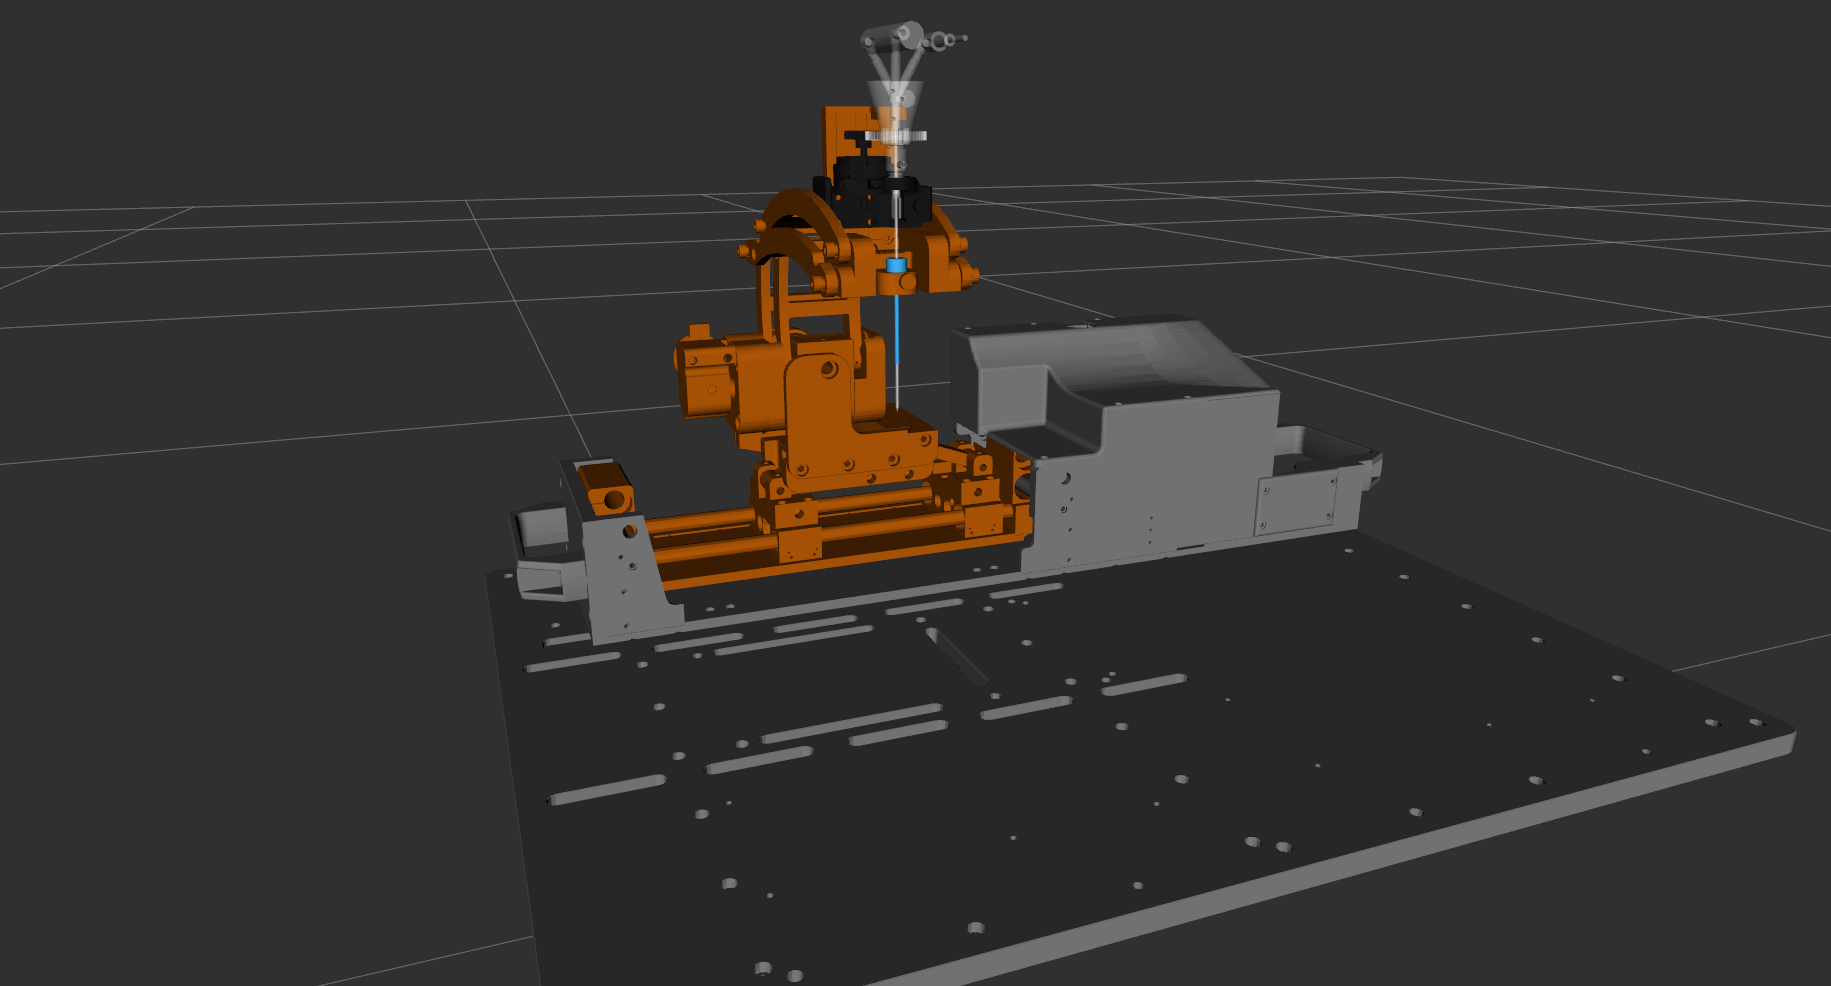
\includegraphics[width=0.7\textwidth]{images/rviz_screenshot_2018_model_needle_in_iso.png}\label{fig:f1}}
  \hfill
  \subfloat[Joint state publisher GUI for active 7 DOF.]{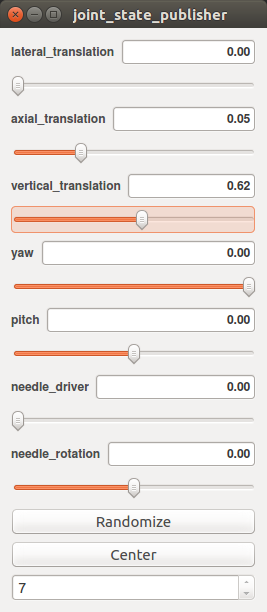
\includegraphics[width=0.2\textwidth]{images/joint_states.png}\label{fig:f2}}
    \caption{End result of neurobot modeling in ROS.}
    \label{fig:jointStatePublisherGUI}
\end{figure}

\subsection{Transforming Joint Space Representations}
\label{sec:transformJointSpace}
\todo[inline]{Revisit this section when completed.}


\section{MoveIt! Neurobot Configuration}
The MoveIt! Setup Assistant tool was utilized to generate the MoveIt! package for the neurobot. The URDF for the neurobot was selected, and the setup tool loaded the robot and stepped through the process of generating the SRDF that would be used for motion planning. A self-collision matrix was first generated, which tests for collisions between different links to see which links, if any, can have collision checking disabled between them to speed up collision checks. The highest resolution of checks was selected to ensure that there would not be any skipped checks that may cause self collisions.

Planning groups were configured next, which described chains of joints which would be considered as a complete manipulator which motion planning would have to solve for. Two planning groups were created. The first described the full arm, which went from the base frame to the needle tip, which included all seven active degrees of freedom. A second planning group included only the first five degrees of freedom to the needle driver base. This second planning group would simplify motion planning to the entry point, where the needle driver and rotation were not needed to be controlled. 

Planning groups also needed an IK solver to be specified that would be instantiated upon a planning instance. The default IK solver utilized KDL, which was a numerical IK solution capable of solving serial chains and dealing with underconstrained systems. It properly supported the mimic joints within the planning group chain as well but would not always update the joints of the robot outside of the planning group which were mimicing joints within the planning group. This opened up the necessity for some additional workarounds in the workspace analysis and motion planning aspects of the project. 

While the KDL IK solver worked properly, a custom solver implemented with IKFast, which was an analytical solver, could significantly speed the execution of the program. \cite{ikFastMoveIt} OpenRAVE includes IKFast as a plugin, so OpenRAVE was installed as an attempt to quickly generate an IKFast solution for the neurobot. This included converting the neurobot URDF to a COLLADA file using a command line tool and running the IKFast generation using that COLLADA file. Unfortunately, IKFast could not recognize the mimic joints on the robot to generate an analytical solution. As a faster IK solver was seen as an optimization, further work on this front was halted, but eventually including an analytical IK solution for the neurobot could noticeably speed up the workspace analysis and motion planning.

Robot poses could also be specified, which were joint configurations that would be meaningful to drive the robot to in common practice. For the neurobot, the default zero position sufficed. End effectors were also chosen, which were tied to planning groups which controlled them. The needle and cannula were both selected as end effectors for the full arm planning group and driver base planning group respectively. Finally, no virtual joints were created for the robot, but this option existed in the setup assistant. With all of the above options set, the MoveIt! package for the neurobot was generated in the workspace.


\section{Environmental Modeling}
The environment for the neurobot consisted of the MRI scanner bore and the patient head. The MRI bore was exported from a SolidWorks model of the scanner with the bed removed to reduce the polygon count of the STL to speed up collision checking. For testing purposes, the patient head was imported as an STL of a mannequine approximation of a person's head. This was not ideal, but Slicer could later be used to take real patient images \todo{GF:i think you can update that now and say you have done it with an animal subject } and generate an accurate collision model for planning around the patient, as described in \autoref{sec:mriSegmentation}.

These models were loaded into the MoveIt! planning scene over a planning scene monitor to utilize as collision objects for the workspace analysis and motion planning. Using the monitor allowed the collision objects to be added and removed from the world at will and to be manually modified within the MoveIt! RViz plugin. An RViz screenshot the typical planning scene environment is shown in \autoref{fig:mriBore}.

\begin{figure}[thpb]
	\centering
	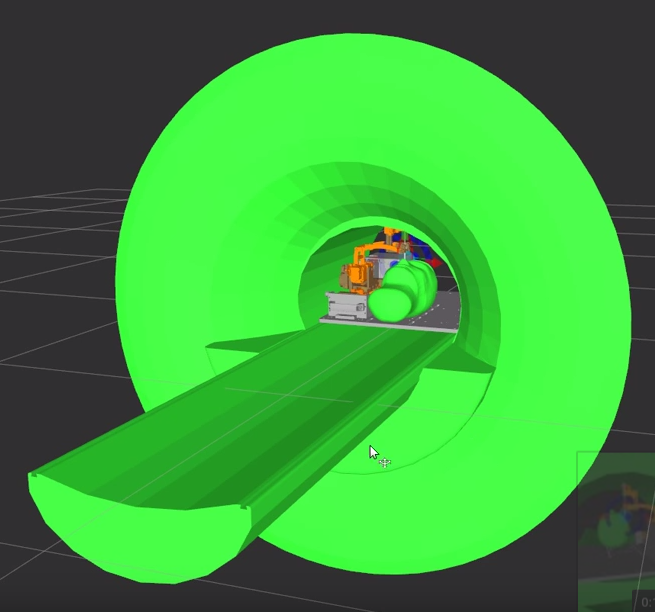
\includegraphics[width = 4in]{images/mri_bore_and_head.png}
    \caption{An image from RVIZ showing the MRI Bore model and human head model loaded with the robot utilizing the MoveIt! API from within a C++ node.}
    \label{fig:mriBore}
\end{figure}


\section{System Interaction and Visualization}
MoveIt! included a plugin for RViz that allowed motion plans to be generated by moving an interactive marker representing the end effector state around the environment while the IK was computed for the robot in real time, showing the actual state of the robot necessary to reach the desired point. A motion plan could then be generated from the current state of the robot to the target state, and if the planning was successful, a preview of the trajectory was played on a loop on the robot model. The interface also allowed collision objects to be loaded from STL's or added and removed once they were published to the planning scene monitor, as discussed in the previous section. \autoref{fig:moveItRViz} shows the MoveIt! plugin being used in RViz.

\begin{figure}[thpb]
	\centering
	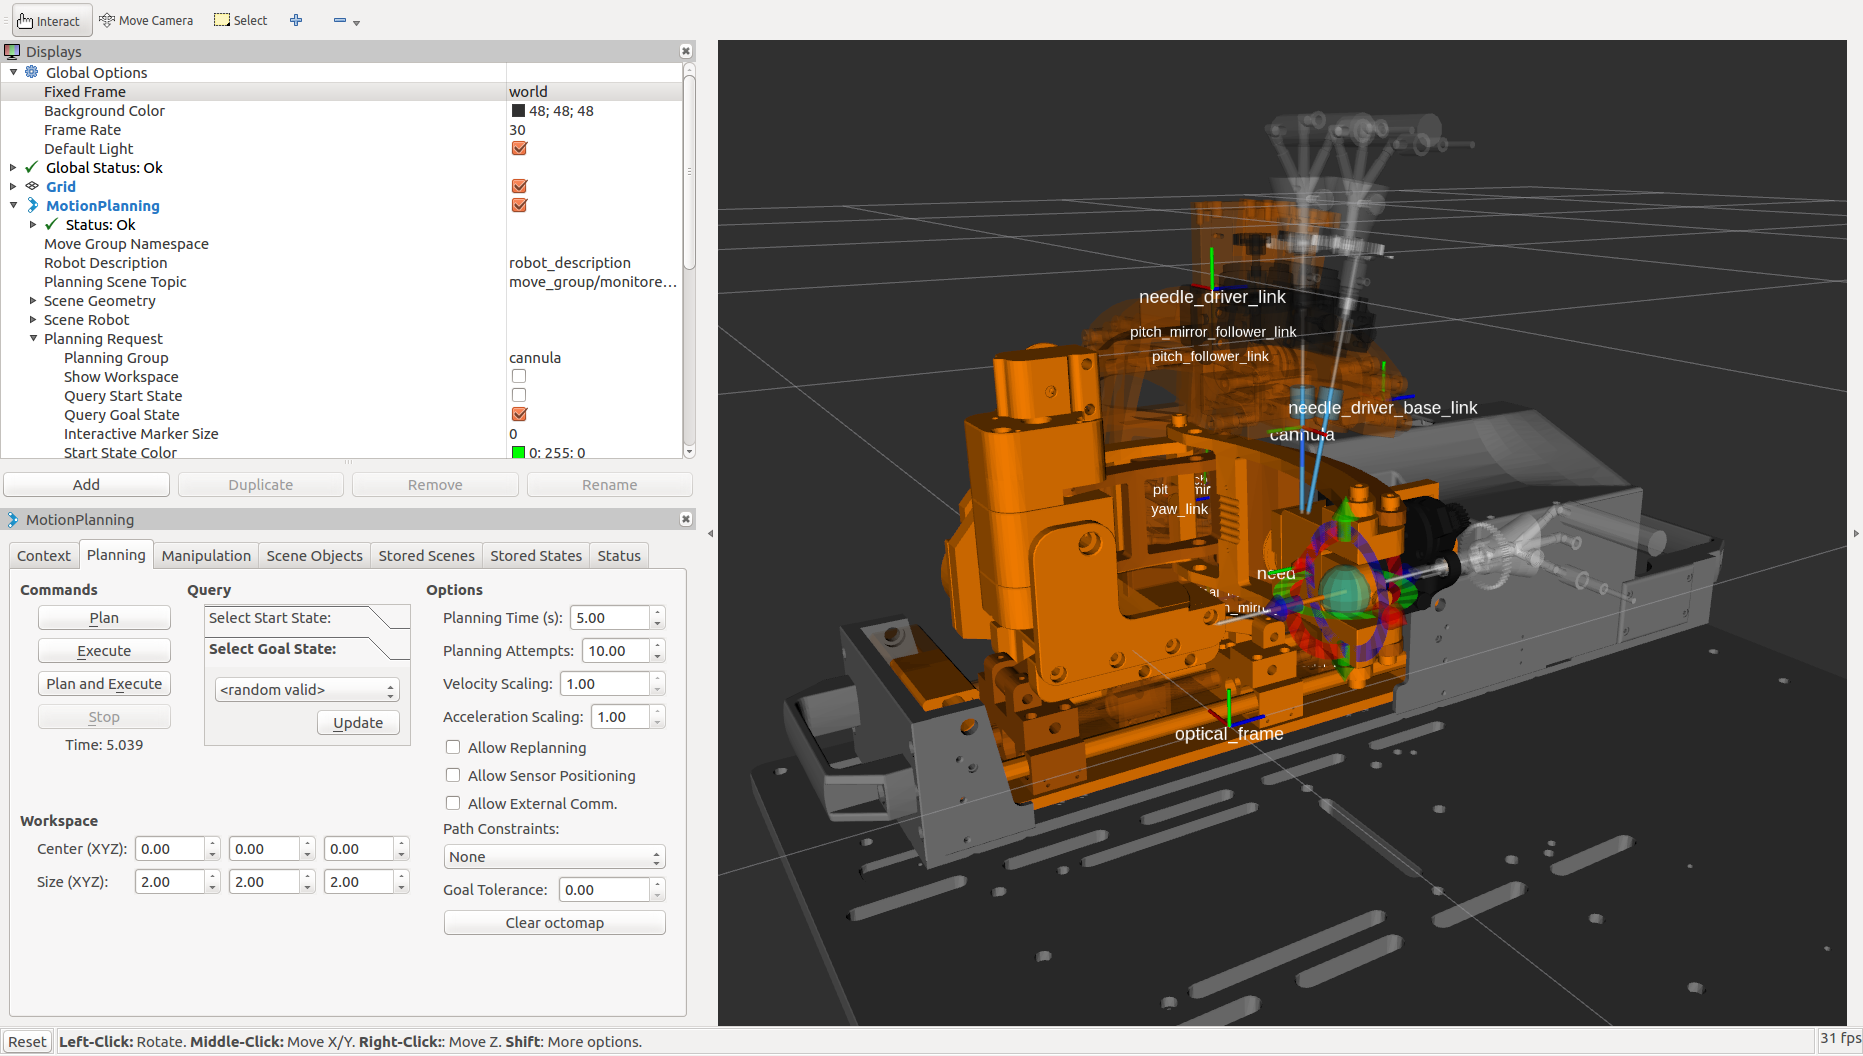
\includegraphics[width=\textwidth]{images/moveit_rviz_plugin_neurobot.png}
    \caption{Screenshot of RViz with the MoveIt! plugin enabled for the neurobot. A trajectory has just been found to the state with the brightly-colored model of the neurobot.}
    \label{fig:moveItRViz}
\end{figure}


%%%%%%%%%%%%%%%%%%%%%%%%%%%%%%%%%%%%%%%%%%%%%%%%%%%%%%%%%%%%%%%%%%%%%%%%%%%%%%%%
\chapter{Workspace Examination}
In this chapter, the work of conducting workspace analysis of the neurobot is discussed. The different components of this objective were visualizing the full entry workspace of the robot, visualizing the workspace of the ultrasonic element, adding collision checks with the environment, and creating the workspace given an entry point. 


\section{Entry Point Workspace Visualization}
The general approach for the workspace visualization was to iterate through the joint space of the robot and use the FK solution to store the end effector position in a list which was then published as a point cloud. In this step of the process, the workspace of valid entry points was generated. The entry point was based on the inputted offsets, discussed in \autoref{sec:neuroablationProcedures}, and the first five DOF of the robot were sufficient to resolve this. A discrete linear space was created between the joint limits on each of the five active joints, and this space was then iterated through to fully explore the robot's available workspace. 

Self-collisions between links had to be checked, and this proved to require some careful use and updating of the planning scene that was storing the robot state. The general process was to load the kinematic model of the robot and the planning groups defined using MoveIt!, and use the planning scene to update a virtual robot with new joint values, test for self collisions, and based on the result, add the reachable end effector point to the list of reachable workspace points.

Issues arose with simply using the active planning group for the workspace analysis; setting the planning group joint limits did not update the full kinematic state of the robot. In most applications, this is desirable, but for the Neurobot, the changes in the serial chain needed to be mimiced by the other joints in the robot to check that the state was valid. This was resolved by algorithmically detecting the active degrees of freedom of the robot from the entire kinematic model, storing their names in order, and then rather than updating the planning group joint values, the active joint values for the entire robot were updated and the Robot State API would update any mimicing joints as necessary in the entire robot's kinematic model. Better support for mimic joints in MoveIt!, especially with the planning groups, would have simplified much of the development of this node, but even with these limitations, the entry workspace of the robot was successfully generated as a point cloud and wrapped with a mesh that was viewable in Slicer, as shown in \autoref{fig:entryWorkspace}.

\begin{figure}[thpb]
	\centering
	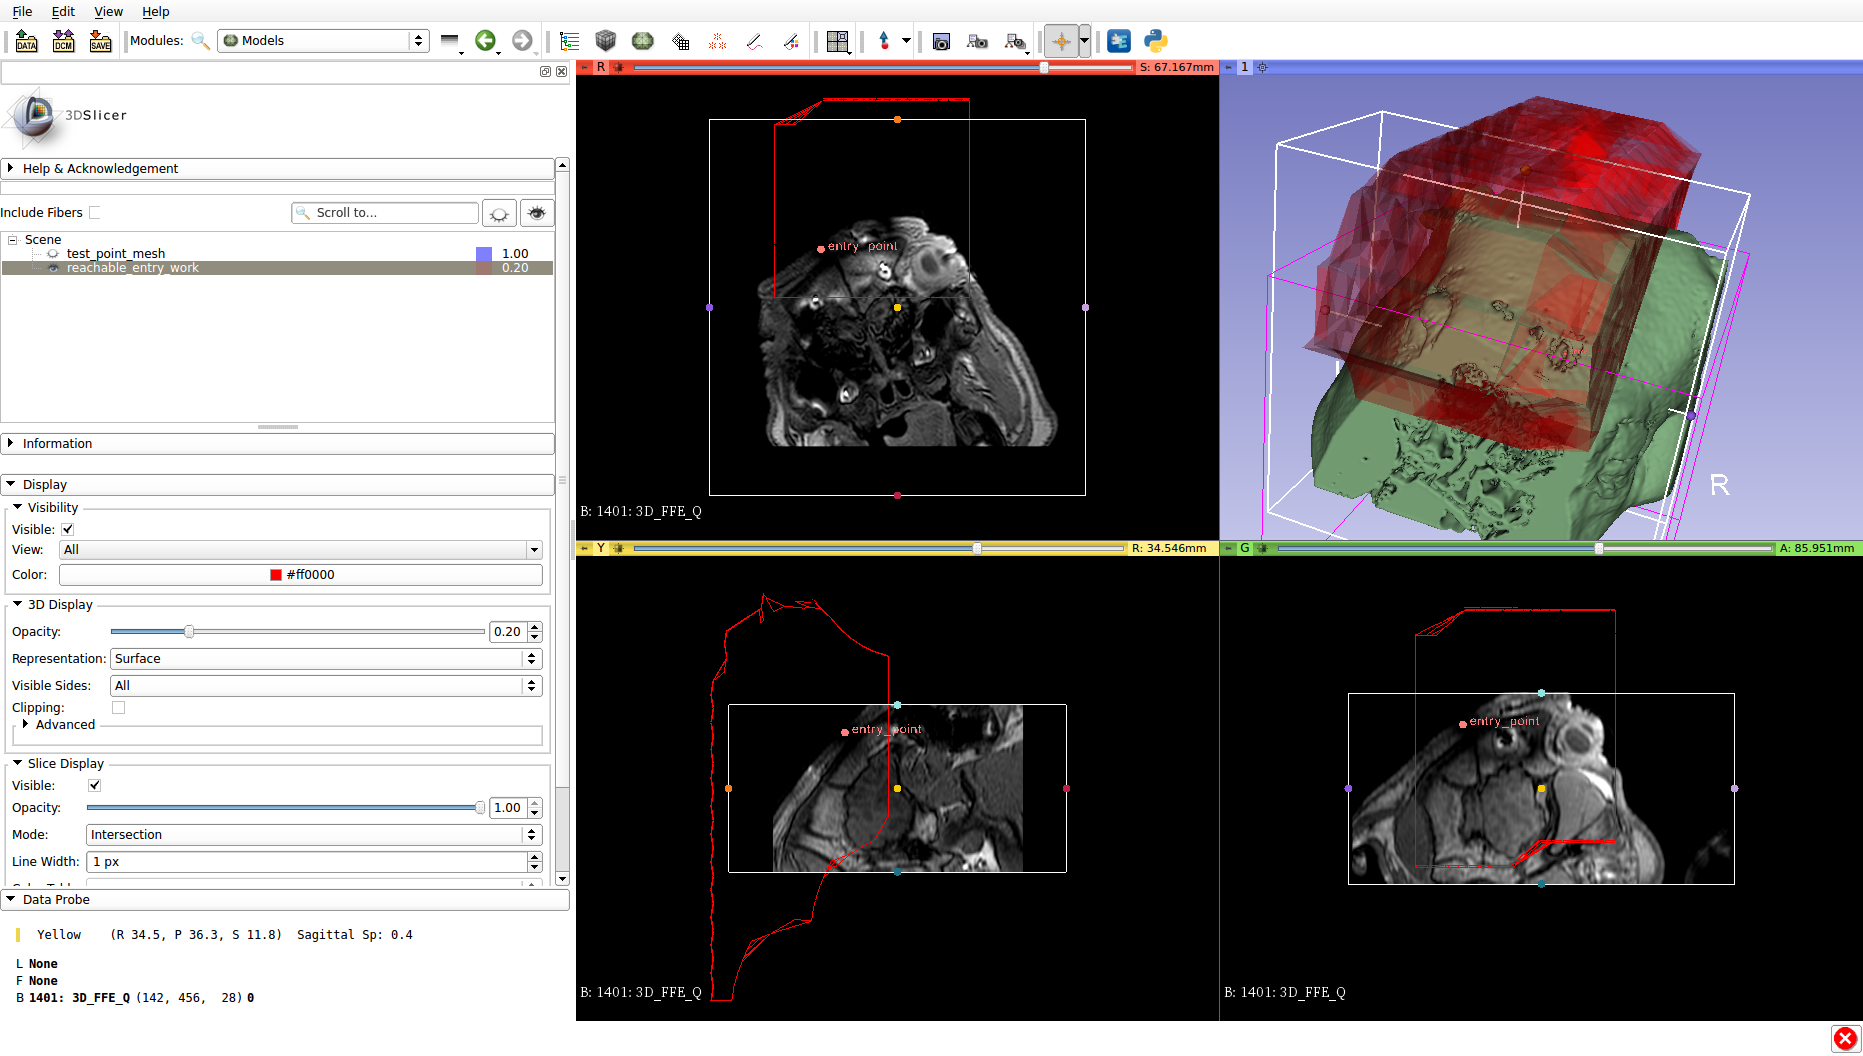
\includegraphics[width=\textwidth]{images/slicer_entry_workspace}
    \caption{Screenshot of Slicer with the entry workspace mesh overlaid on a pig head.}
    \label{fig:entryWorkspace}
\end{figure}


\section{Element Workspace Visualization}
The ultrasonic element on the probe was essentially the true end effector of the robot. For determining the element workspace of the robot, the same process described for the entry workspace was used, but including the additional DOF provided by the needle driver. The needle rotation was ignored since it would not move the element workspace, but it is possible the geometry of the cooling tubes could allow needle rotations to have a slight impact on the workspace. In the future, since it would be desirable to have the ability to spin the needle for conducting treatments using a non-symmetric ultrasonic probe. 

Since a fixed-length needle based on the SolidWorks model of the robot was used and the actual offsets could change to accommodate different probes, this was compensated for while iterating the needle DOF through its range of motion. In the future, this could instead be handled by having a set of different probe models which could be placed on the robot as end-effectors, making the process more generic and adaptable. The cannula length could also change, so a check was made to ensure that the ultrasonic element would be exposed beyond the cannula to be considered a valid position. If the ultrasonic element of the probe was still within the cannula, the ablation and possibly the probe could fail. However, it was also possible to adjust the cannula manually to achieve the desired size, so this was not particularly critical to operations. \autoref{fig:elementWorkspace} shows the generated workspace as shown in Slicer.

\begin{figure}[thpb]
	\centering
	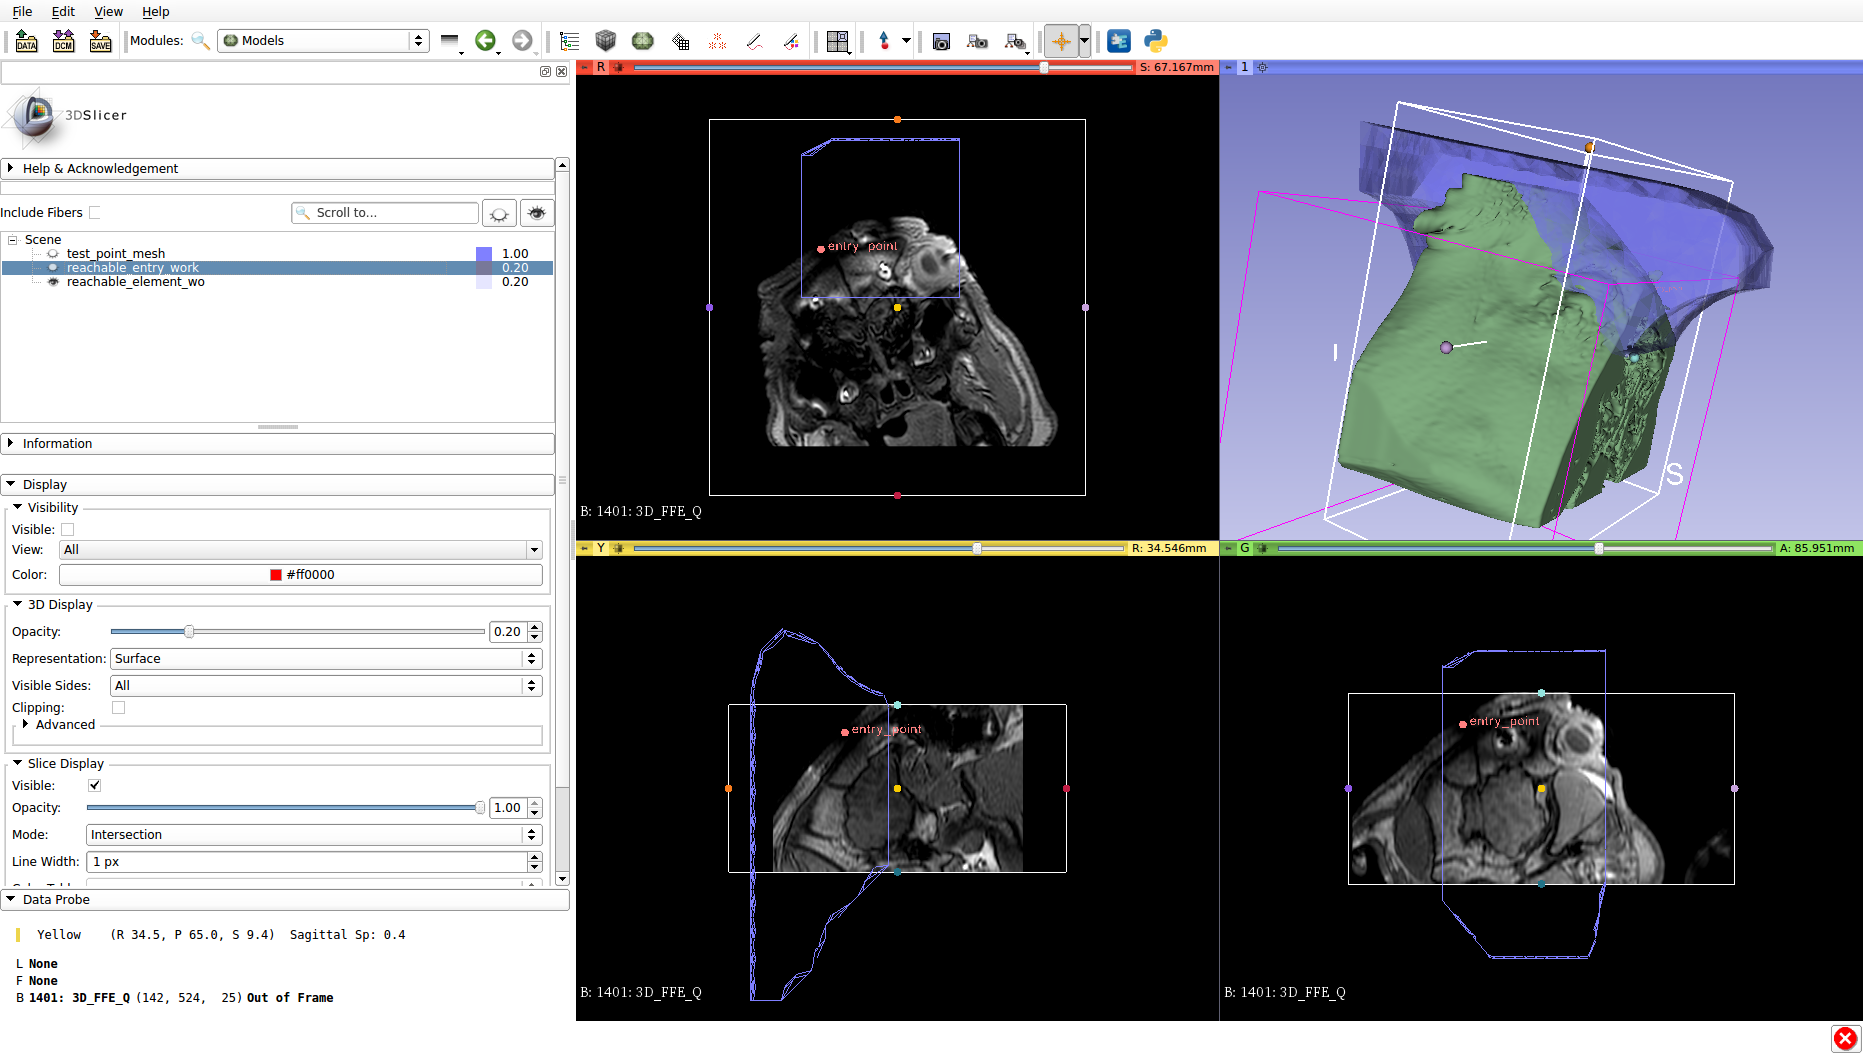
\includegraphics[width=\textwidth]{images/slicer_element_workspace.png}
    \caption{Screenshot of Slicer with the ultrasonic probe element workspace mesh overlaid on a pig head.}
    \label{fig:elementWorkspace}
\end{figure}


\section{Collision-Aware Workspace Examination}
Collision checking was added somewhat easily to the process of generating the workspace. Collisions with the environment could be checked by publishing collision objects to the planning scene. For the full workspace of the robot, collision checks with the MRI scanner bore were necessary. The STL model of the bore was loaded by file path and published to the planning scene monitor, such that the internal scene in the node included the scanner and the published planning scene in ROS also had access. \autoref{fig:rvizEntryWorkspaceBore} shows the view in RViz with the scanner bore loaded and the entry workspace generated with collision checking with the bore.

\begin{figure}[thpb]
	\centering
	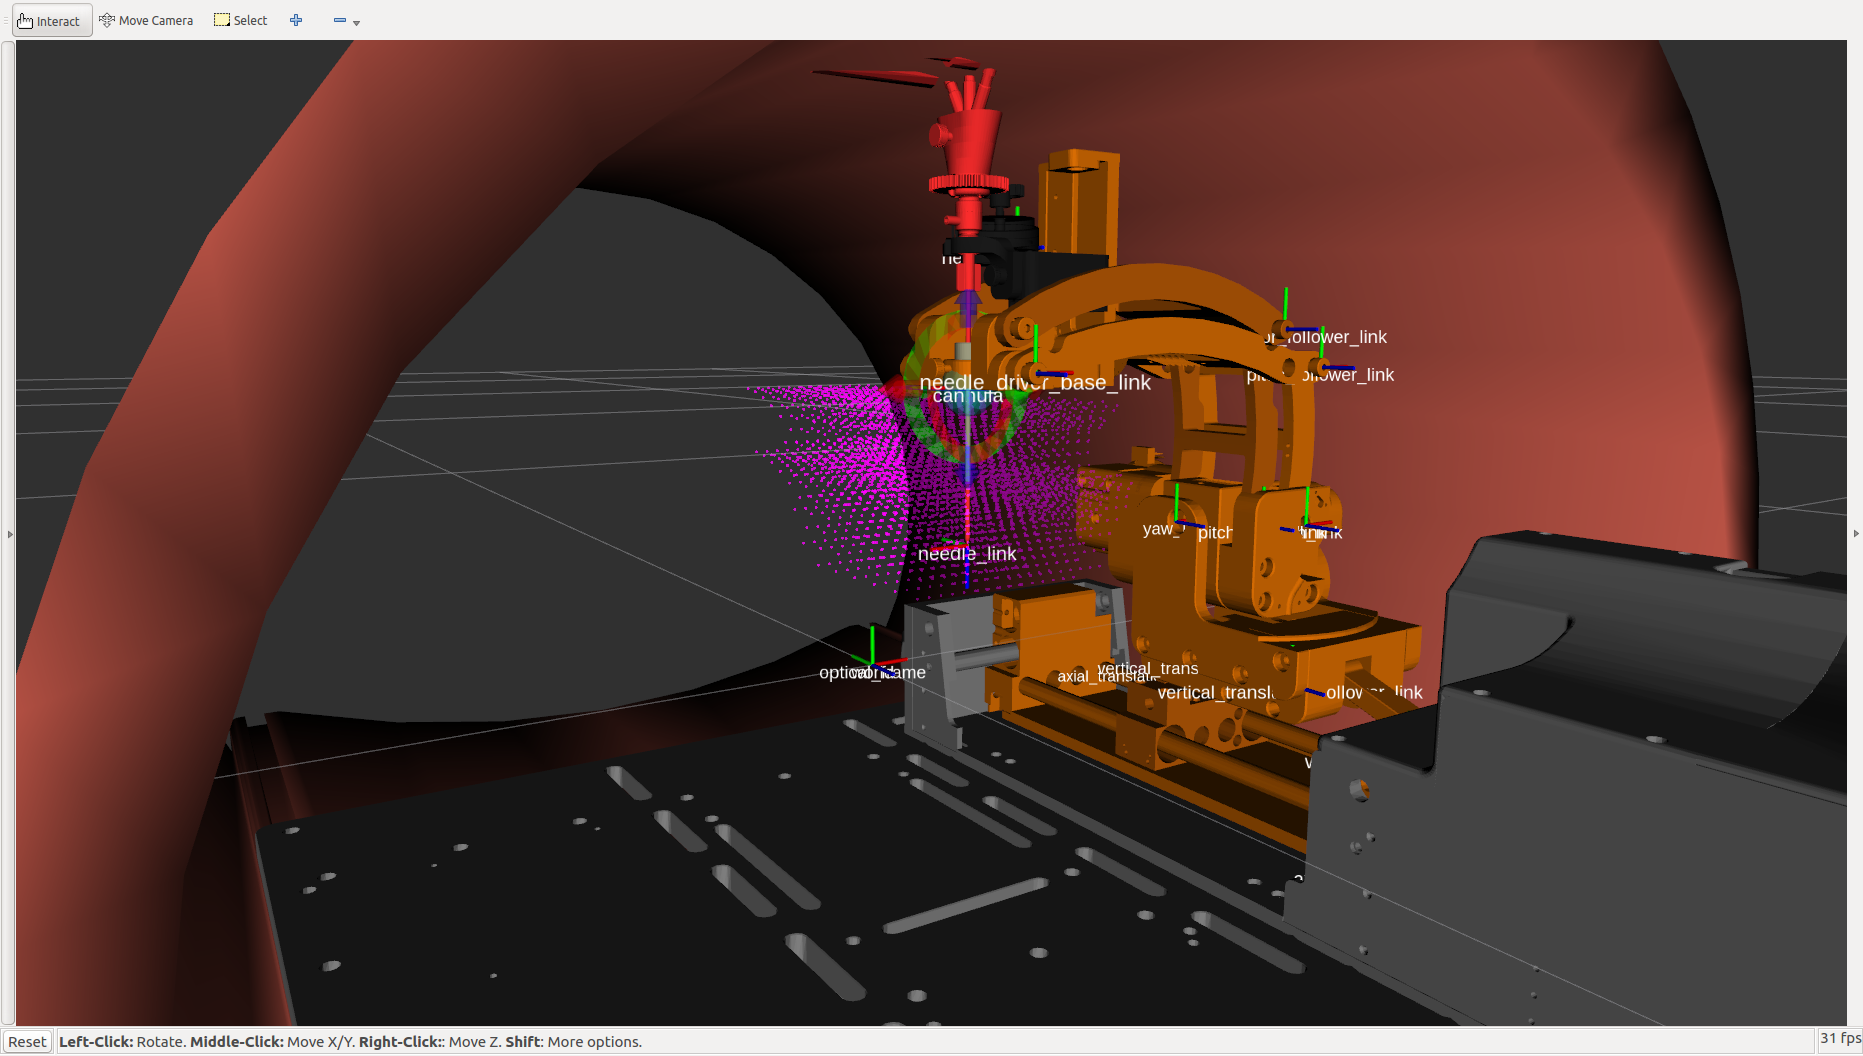
\includegraphics[width=\textwidth]{images/rviz_entry_workspace_bore.png}
    \caption{Screenshot of RViz with the scanner bore loaded in the planning scene and the entry workspace computed as a point cloud.}
    \label{fig:rvizEntryWorkspaceBore}
\end{figure}

The above two features were then modified to accept a collision checking function to allow flexible collision checking with either just self-collision checks or environmental checks. To speed up full collision checks, self-collisions were first checked since these were sped up by the self-collision matrix created during MoveIt! setup. If a self collision happens, then environment collision checks are skipped and the next configuration is tested. However, if the self-collision check passes, then collision checks with the environment are performed. \autoref{fig:entryAndElemeWorkspaceCollision} shows the entry and element workspaces in Slicer with the collisions with the scanner bore considered.

\begin{figure}[thpb]
	\centering
	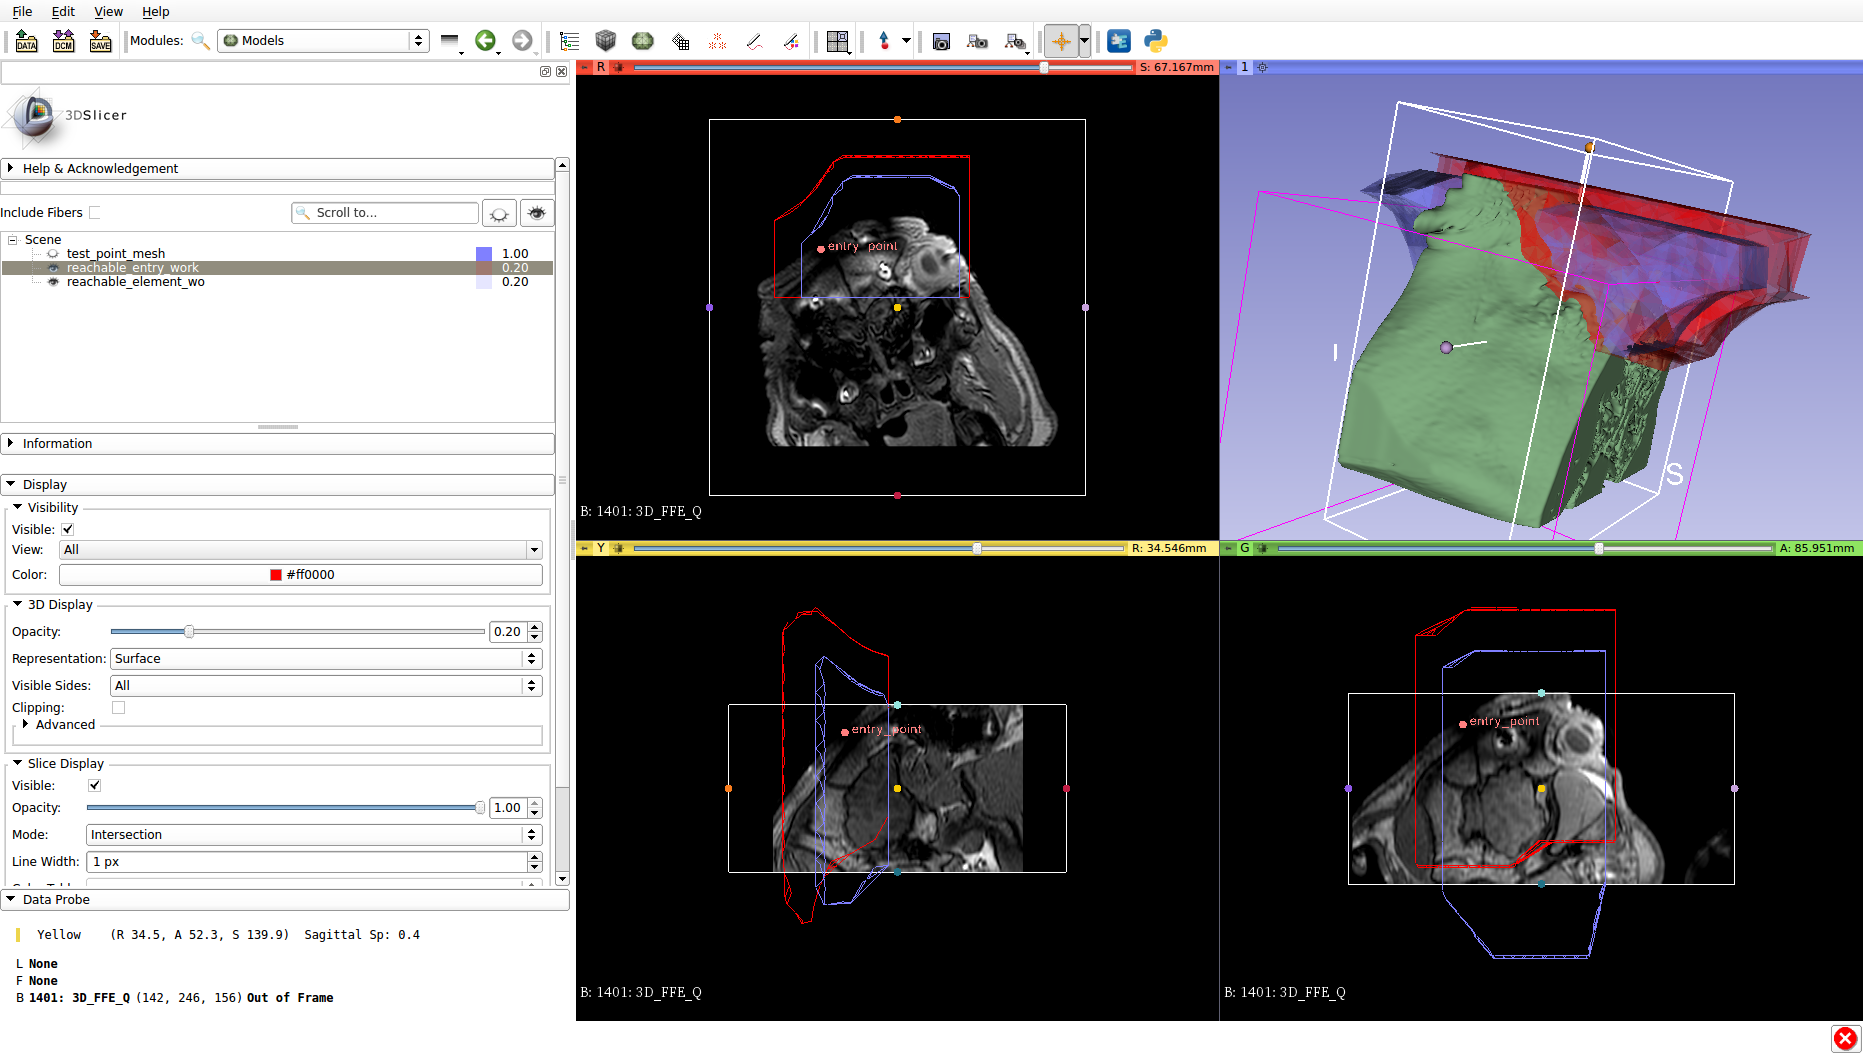
\includegraphics[width=\textwidth]{images/slicer_entry_and_elem_with_bore.png}
    \caption{Screenshot of Slicer with the entry point and element workspace meshes overlaid on a pig head considering collisions with the scanner. Red mesh is entry; blue is element.}
    \label{fig:entryAndElemeWorkspaceCollision}
\end{figure}


\section{Workspace Evaluation from Entry Point}
The final workspace that was evaluated was that of the element given an entry point for the robot. This analysis was a bit different from the previous two. Essentially, the IK was solved for the first five DOF of the robot to the entry point (with the given robot to entry offset from the entry point to the robot's cannula base) by iterating through valid rotations at that point, and when a configuration was found that solved the IK, collisions were checked and the needle joint was swept through its joint space. In order to speed up collision checking, when an IK solution was found, the needle was kept at the maximum depth so that if collisions occurred at this configuration, they would definitely still occur when the needle was retracted and those tests could be skipped.

While it was desired that the approach would be fairly generic and explore all 3 DOF of rotation, the IK solver was too slow for exploring spaces that were known to be invalid given the kinematics of the neurobot. This was due in part to the numerical nature of the IK solver - an IK solution really was a searching process, so failure to find a solution occurred at a user-specified timeout. This was typically set to around 10ms from experimentation, since a solution could be found for valid configurations within that time on a laptop with an i7-4702MQ processor.  Using an analytical solution would allow the full rotational space to be explored to make the solution more generic, but this solution approach worked well and could generate an accurate workspace in about 40 seconds for an entry point, the result of which can be seen in \autoref{fig:elementWorkspaceEntryPoint}.

\begin{figure}[thpb]
	\centering
	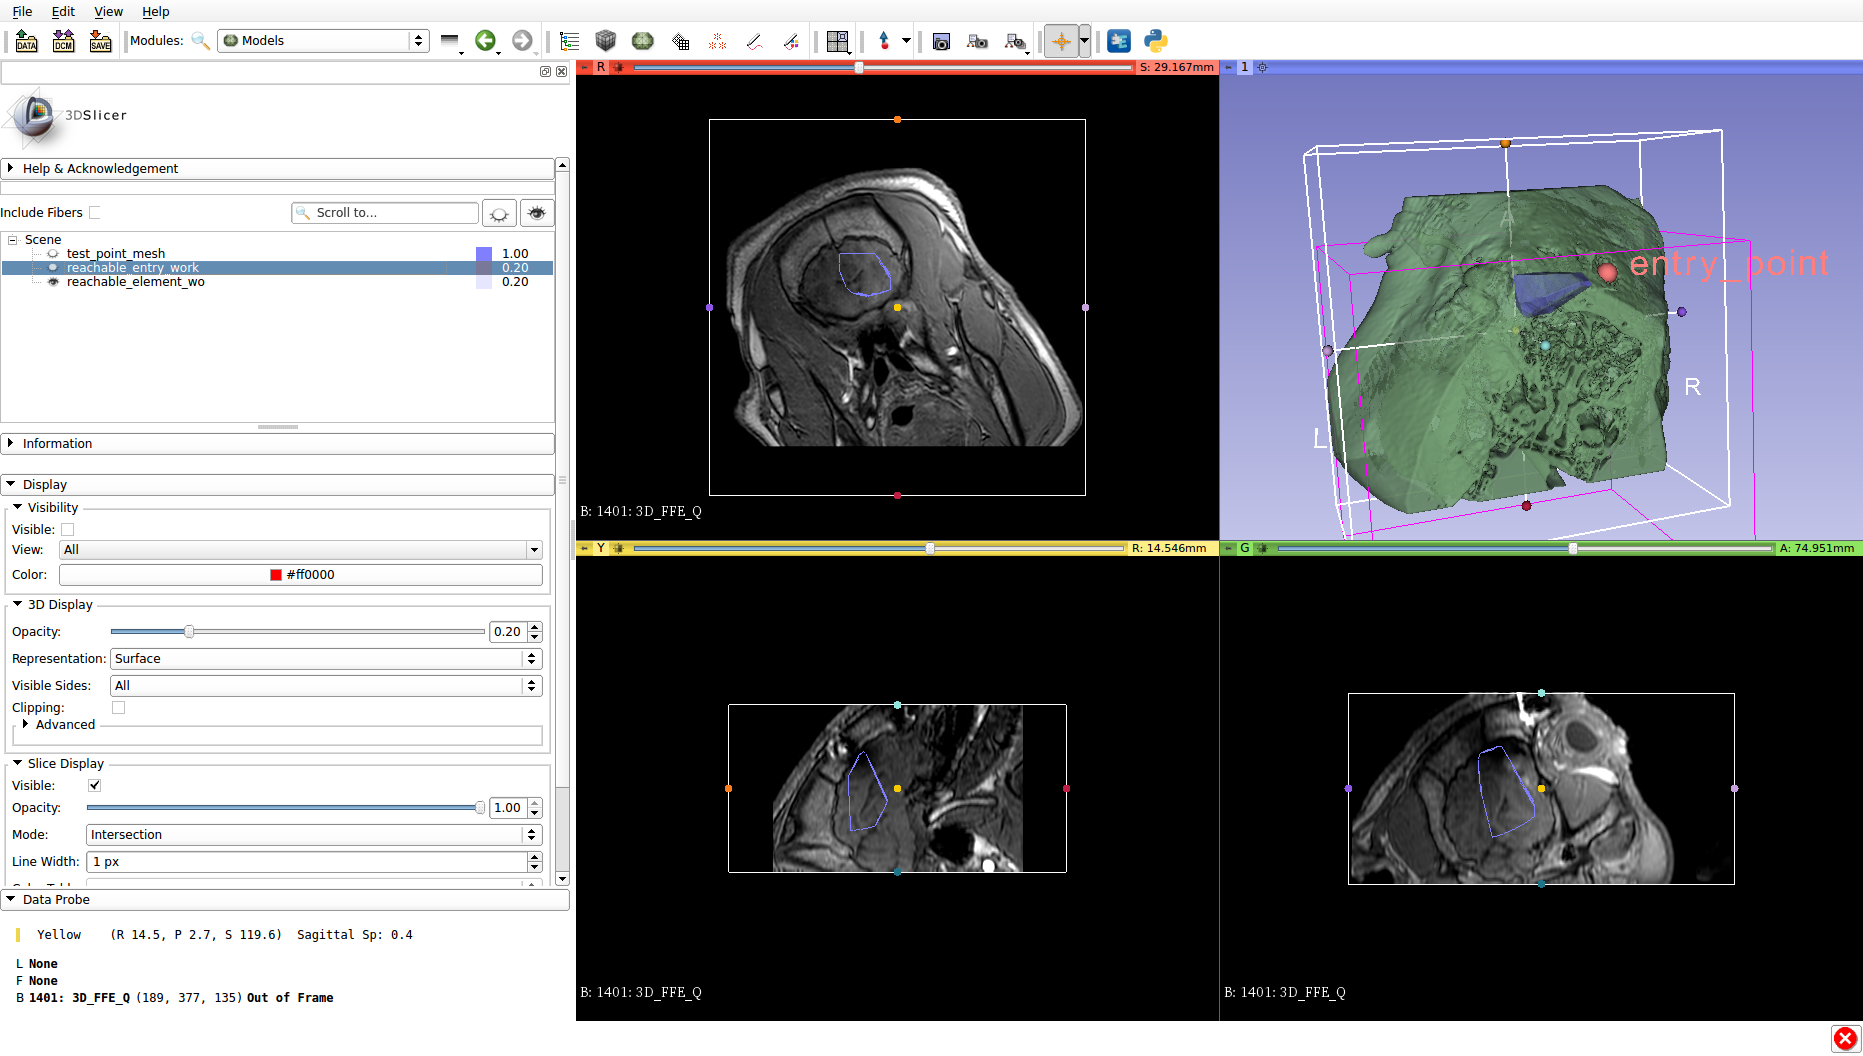
\includegraphics[width=\textwidth]{images/slicer_workspace_given_entry.png}
    \caption{Screenshot of Slicer with the ultrasonic probe element workspace given an entry point.}
    \label{fig:elementWorkspaceEntryPoint}
\end{figure}


\section{Selecting the Target Point}
With the workspace of the probe element shown in Slicer given the entry point in the patient head, the user could then select the target point. Guided by this workspace, it was clear whether the target point was reachable by the robot and how far the robot could treat within the patient's head with the current burr hole. \autoref{fig:targetPointSelectedInSlicer} shows the target point selected within the allowable workspace of the ultrasonic element on the probe.

\begin{figure}[thpb]
	\centering
	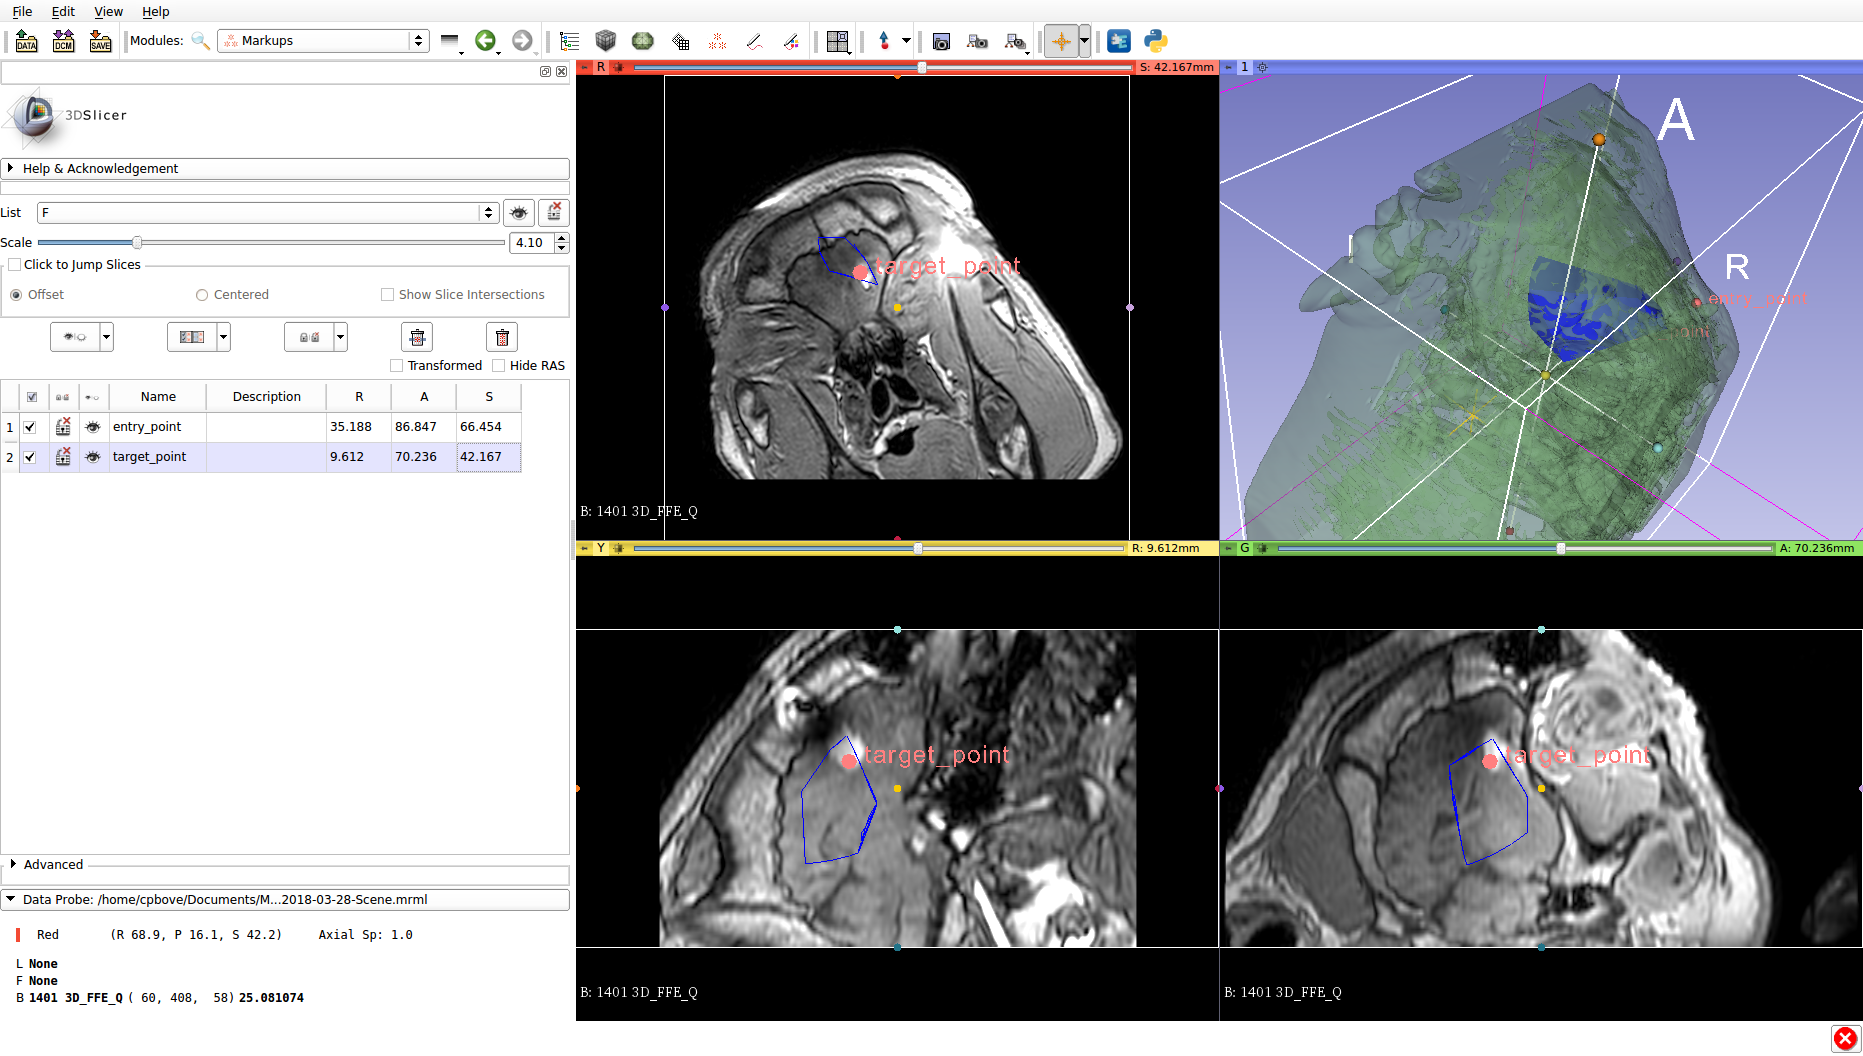
\includegraphics[width=\textwidth]{images/slicer_target_point_selected.png}
    \caption{Screenshot of Slicer showing the target point selected within the workspace allowable by the entry point.}
    \label{fig:targetPointSelectedInSlicer}
\end{figure}

The target point was then sent back over OpenIGTLink to ROS. This would allow ROS to resolve the entry point into an entry pose upon which a motion planning solution could be found. \autoref{fig:rviz_target_and_entry.png} shows an image from RViz of the target and entry point as standard ROS point stamped messages.

\begin{figure}[thpb]
	\centering
	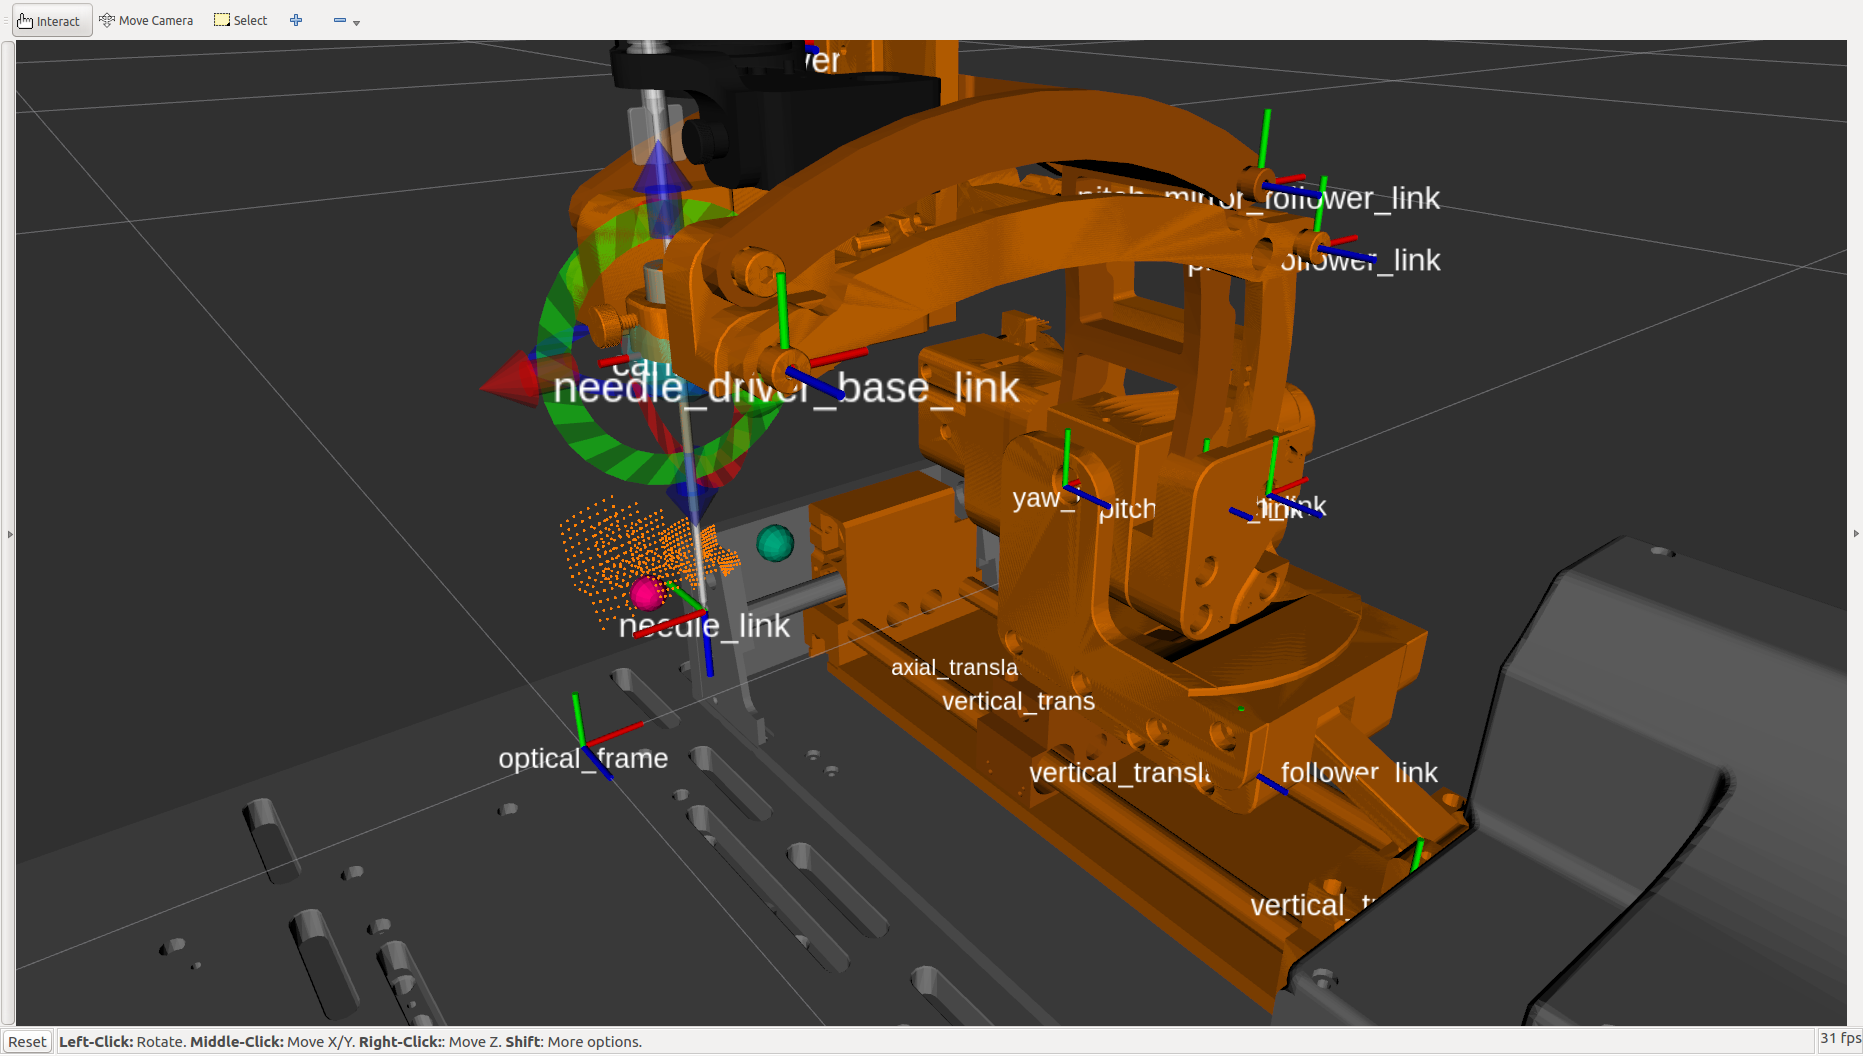
\includegraphics[width=\textwidth]{images/rviz_target_and_entry.png}
    \caption{Graphic from RViz showing the entry point (blue) and the target point (pink) in the point cloud (orange) representing the reachable element workspace given the entry point.}
    \label{fig:rviz_target_and_entry.png}
\end{figure}


%%%%%%%%%%%%%%%%%%%%%%%%%%%%%%%%%%%%%%%%%%%%%%%%%%%%%%%%%%%%%%%%%%%%%%%%%%%%%%%%
\chapter{Motion Planning}
For this part of the system development, the MoveIt! API was used within a ROS node to solve the motion planning problem of moving the robot to the entry point without colliding into the patient head to achieve a pose which allowed the target point to be reached by the ultrasonic element on the probe. Once the trajectory was generated, it was transformed into the joint space of the actual robot, and the trajectory was then sent through OpenIGTLink to Slicer, \todo{GF: was it, i didnt see this yet?} where the path was examined and allowed to be executed on the robot controller. The following sections in this chapter discuss the development of these capabilities.  


\section{Motion Planning with MoveIt!}
\subsection{Resolving Entry Pose}
In order for a motion plan to be generated to the entry point that reaches the target point once the ultrasonic probe is added and inserted, the entry point must be resolved into an entry pose in order for the IK to solve for a configuration and the motion planner to have a goal configuration to reach. This was achieved by using both the entry point and the target point to resolve an orientation that could be combined with the entry point to get a full 6 DOF pose. Of course, two 3D points could only resolve two degrees of rotational information, but the last degree (the rotation about the needle) was not needed for the five joints that moved the robot to the entry point and could be determined by the kinematic constraints of the five DOF system in that case. 

\todo[inline]{include psuedocode once finished.}

\subsection{Updating Robot State and Environment}
Motion planning to the entry point also required the current state of the robot, which was attained as described in \autoref{sec:receivingRobotState}. The node simply subscribed to the joint state publisher for the robot and updated the planning scene's robot state with the latest information before starting the motion plan. The patient head was also added as a collision object as provided by the MRI segmentation into a volume as detailed in \autoref{sec:mriSegmentation}, or alternatively motion planning could be conducted on a generic head shape if the patient model was not available. \autoref{fig:motionPlanningSetup} shows the environment setup with the entry point, target point, and patient head mesh for the start of the motion planning process.

\begin{figure}[thpb]
	\centering
	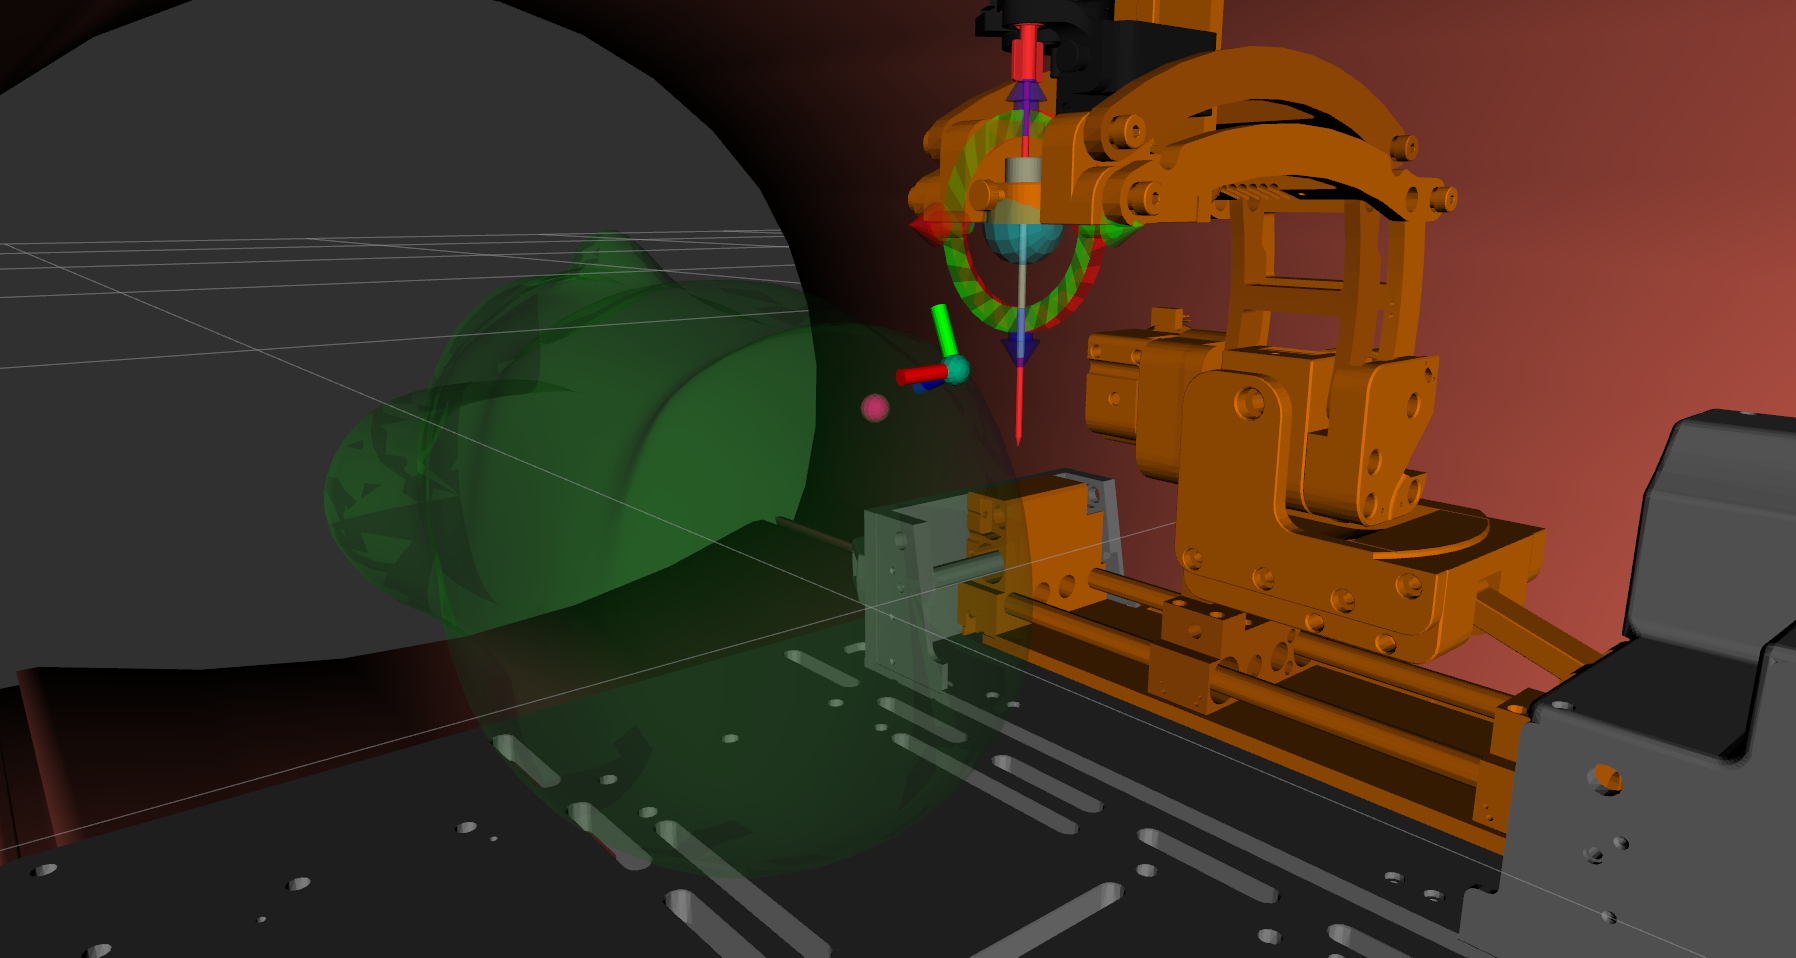
\includegraphics[width=\textwidth]{images/motion_planning_setup_2.png}
    \caption{Screenshot from RViz showing the motion planning setup for finding a trajectory to the entry pose around the patient head.}
    \label{fig:motionPlanningSetup}
\end{figure}

\subsection{Checking Collisions and Assumptions}
As review, the robot remained outside of the MRI bore and did not have the ultrasonic probe and cannula installed when the robot was sent to the entry point during procedures. This allowed the robot to move without the additional constraints of the probe and cannula potentially hitting the patient head and the rest of the robot striking the MRI bore. However, once the robot moved to the entry point, the needle driver was added and inserted to the required depth, and the patient bed was slid into the MRI tube for monitoring of the ablation. 

Before beginning the process of motion planning, it was checked to see if an IK solution could be found to bring the robot to the required entry pose and if that configuration (with the needle inserted to achieve the target point) avoided collisions with the MRI bore. It could be assumed that the target point was chosen within the allowable workspace given the entry point, but a warning would be thrown if this was a case, requiring an override by the user to continue to generate a solution with the knowledge that the final configuration of the robot would be in a collision state.

With it now known that the entry pose and target point were reachable without collision, the next step of the motion planning process could be completed. Since the robot did not have the cannula and ultrasonic probe installed during movements to the entry point, these links could be ommitted from collision checking. This was accomplished by modifying the Allowable Collision Matrix (ACM) within the MoveIt! planning scene to ignore collisions between the cannula link and the needle/probe link. 

\subsection{Generating a Motion Plan}
With the setup work completed, searching for a motion plan was a relatively straightforward task. This was as simple as calling a function with the MoveIt! API to generate a plan to the entry pose joint configuration. The motion planner then searched for a valid path to the goal, and if the planner timed out, this was considered a failure and the operators would have to manually position the robot. With collisions considered between the robot and patient, trajectories were typically found within 20 seconds, so a 30 second timeout was used for the motion planning problem. It could also indicate that there was no way to move the robot to the entry point without violating its kinematic constraints while avoiding collisions with the patient head, so perhaps a safer response would be to reposition the patient, perform new scans, and begin the process again as shown in the workflow designed in \autoref{sec:surgicalWorkflow}. If the plan was successful, the trajectory was published, and the set of end effector poses was published as well.

As discussed in \autoref{sec:motionPlanning}, LBKPIECE was supported by MoveIt! and produced faster trajectories that other motion planning algorithms. Unfortunately, the MoveIt! wrapper did not expose the ability to manipulate or change cost functions. Thus the default cost function was utilized, which optimized the path distance. Below are the available configuration options and the values chosen for the experiments. \autoref{fig:motionPlanRViz} shows a trajectory being executed within RVIZ given this configuration to move the robot from the current state to the entry pose without striking the patient head, and \autoref{tab:lbkpieceSettings} documents the planner parameters used for the project.

% \begin{table}[htbp]
% \caption{Motion planner settings for LBKPIECE.}
% \label{tab:lbkpieceSettings}
% \vskip6pt
% \centerline{
% 		\singlespacing
% 		\begin{tabular}{|p{3cm}|p{2cm}|}
% 		\hline
% % 		\bf{Parameter Name} & \bf{Value} \\ \hline
% % 		Border Fraction & 0.9 \\ \hline
% % 		Failed Expansion Goal Factor & 0.5 \\ \hline
% % 		Goal Bias & 0.9 \\ \hline
% % 		Min Valid Path Fraction & 0.5 \\ \hline	
% % 		Border Fraction & 0.9 \\ \hline
% % 		Min Valid Path Function & 0.5 \\ \hline
% % 		Range & 0.0 \\ \hline
% % 		Type & Geometric KPIECE \\ \hline
% 		\end{tabular}
% 		\doublespacing
% 	}
% \end{table}

\begin{table}[htbp]
\caption{Motion planner settings for LBKPIECE.}
\label{tab:lbkpieceSettings}
\vskip6pt
\centerline{
		\begin{tabular}{|p{3cm}|p{2cm}|}
		\hline
		\bf{Parameter Name} & \bf{Value} \\ \hline
		Border Fraction & 0.9 \\ \hline
		Failed Expansion Goal Factor & 0.5 \\ \hline
		Goal Bias & 0.9 \\ \hline
		Min Valid Path Fraction & 0.5 \\ \hline	
		Border Fraction & 0.9 \\ \hline
		Min Valid Path Function & 0.5 \\ \hline
		Range & 0.0 \\ \hline
		Type & Geometric KPIECE \\ \hline
		\end{tabular}
	}
\end{table}

\begin{figure}[thpb]
	\centering
	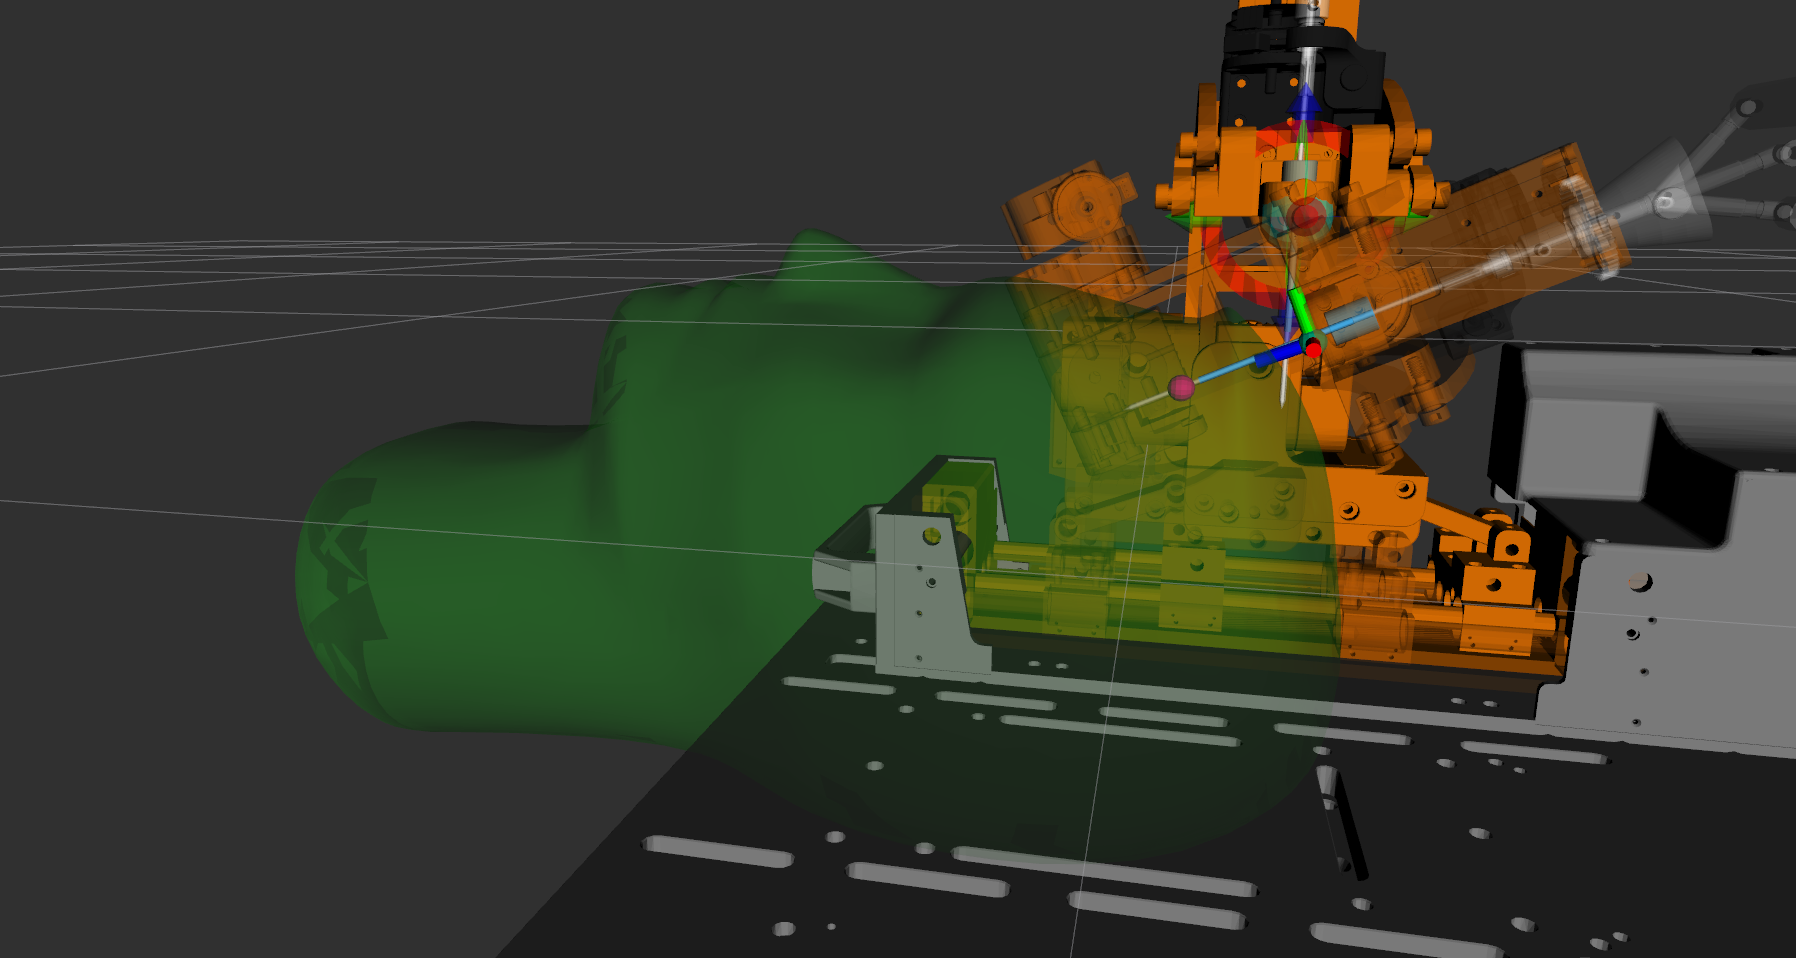
\includegraphics[width = \textwidth]{images/motion_plan_rviz.png}
    \caption{RViz screenshot of the trajectory solution showing the starting and ending state of the robot. An looped animation plays showing the robot following the trajectory.}
    \label{fig:motionPlanRViz}
\end{figure}


\section{Transform Joint Space Trajectories}
Essentially, the same tools used for converting the joint space as discussed in \autoref{sec:receivingRobotState} was utilized for this step as well, which took place in a different node. Each joint state was transformed using the inverse functions applied to convert the real robot's joint state into the modeled version in ROS. Once this transformation occurred, the node published the  The velocities chosen for the modeled joints were matched previously during the URDF creation to ensure velocities would be attainable for the real robot hardware as well. Of course, the robot controller had the capability of slowing down the movements further in order to make sure that all the joints reached the desired setpoint for each step of the trajectory. 


\section{Trajectory Control in Slicer}
A final check of the validity of the motion plan was performed in Slicer. The end effector path was converted by a ROS node into a OpenIGTLink polydata object that contained the series of lines connecting the points of the path, as illustrated in \autoref{fig:motionPlanSlicer}. This allowed a final sanity check to make sure that the trajectory reached the entry point in a reasonable way and would avoid hitting the patient. Once this was confirmed, the trajectory was allowed to be executed on the robot by using the interface provided on the robot controller software and pressing the foot pedal.

\begin{figure}[thpb]
	\centering
	%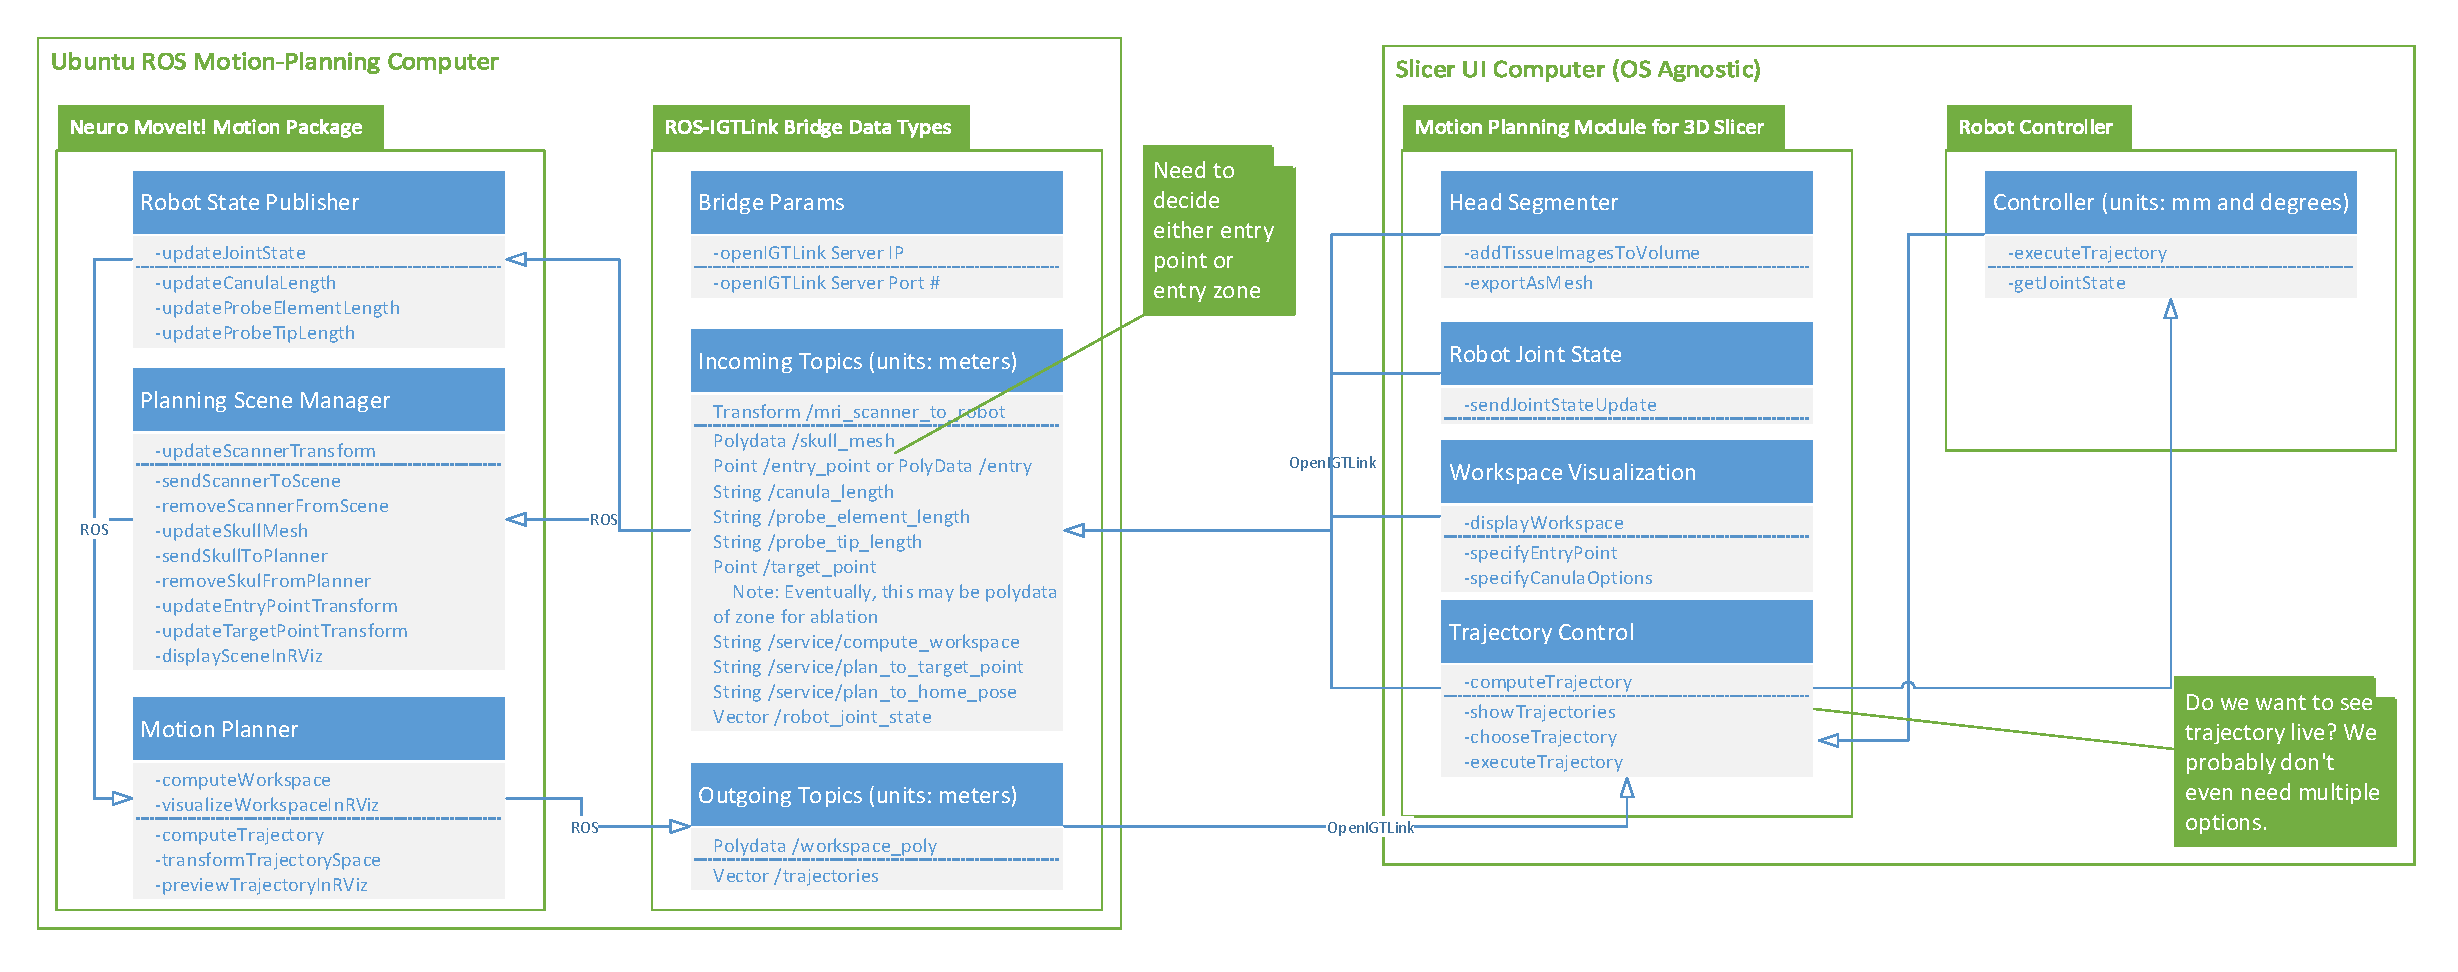
\includegraphics[width=\textwidth]{diagrams/Software_Diagrams.pdf}
    \missingfigure[figwidth=4in]{Screenshot in Slicer of planned path}
    \caption{Screenshot of Slicer showing the end effector path from the motion planning solution.}
    \label{fig:motionPlanSlicer}
\end{figure}


%%%%%%%%%%%%%%%%%%%%%%%%%%%%%%%%%%%%%%%%%%%%%%%%%%%%%%%%%%%%%%%%%%%%%%%%%%%%%%%%
\chapter{MRI Segmentation}
\label{sec:mriSegmentation}
\todo[inline]{GF: maybe we should try on a real human head as well, i believe there are datasets available online. I think we may even have some from dr pilitsis from early in the project.}
In order to have an accurate collision model of the patient head for motion planning, a 3D mesh of the patient head was extracted from available MRI scans and sent over OpenIGTLink to the ROS network for further processing and loading into the planning scene monitor. The following two sections describe this process in more detail.


\section{Slicer Processing}
The process of generating a solid mesh from a series of scans within Slicer was generally straightforward with the Segment Editor. A segment was added using the thresholding tool with the lower bound set to a number which just eliminated the background from the image and the upper bound set to the maximum. \autoref{fig:segmentationThreshold} shows the scan planes with the threshold mask and the rendered 3D volume. \todo{cite}

\begin{figure}[thpb]
	\centering
	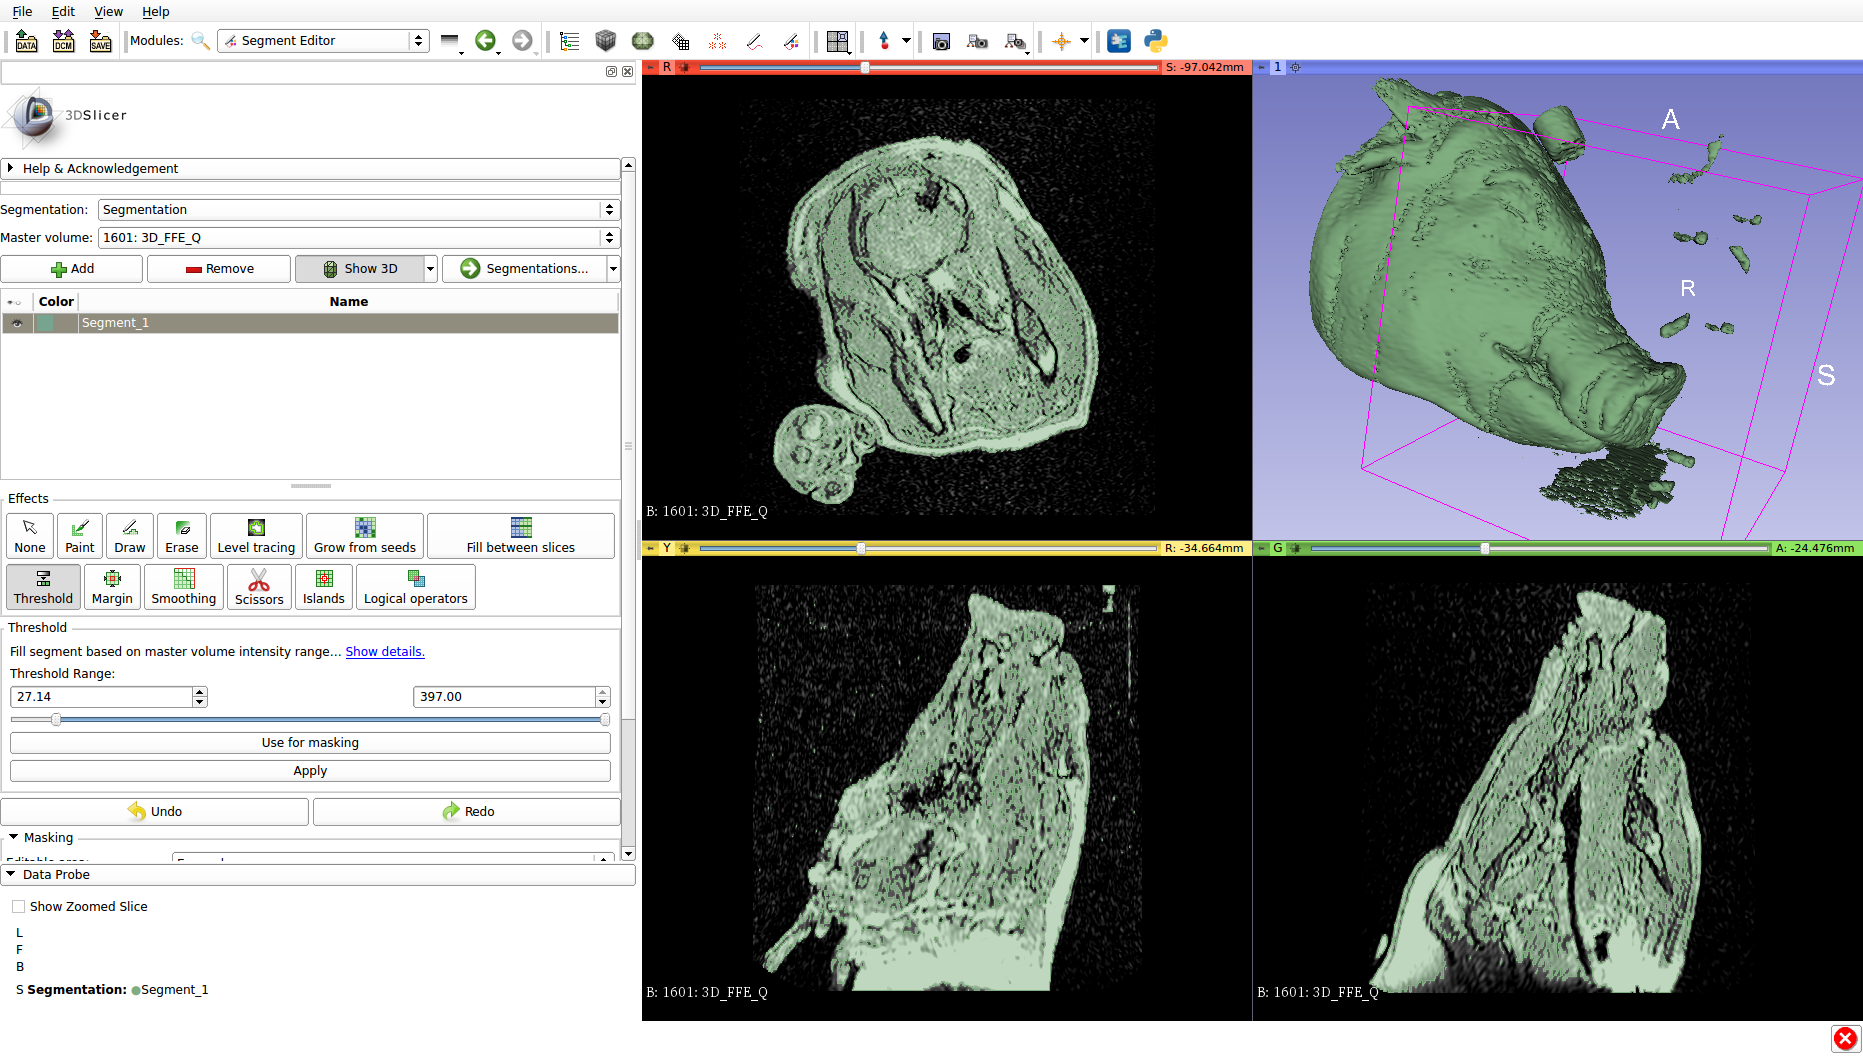
\includegraphics[width=\textwidth]{images/segmentation_threshold.png}
    \caption{Screenshot of Slicer showing the rendered mesh of the patient head based on mask thresholding.}
    \label{fig:segmentationThreshold}
\end{figure}

Once this mask was applied, the islands tool was used to remove all but the largest islands from the selection, which eliminated noise in the image and any items which were visible in the scan but not connected to the largest object, which was the patient's head. The rendered 3D volume is shown in \autoref{fig:slicerHeadMeshNoFilter}.

\begin{figure}[thpb]
	\centering
	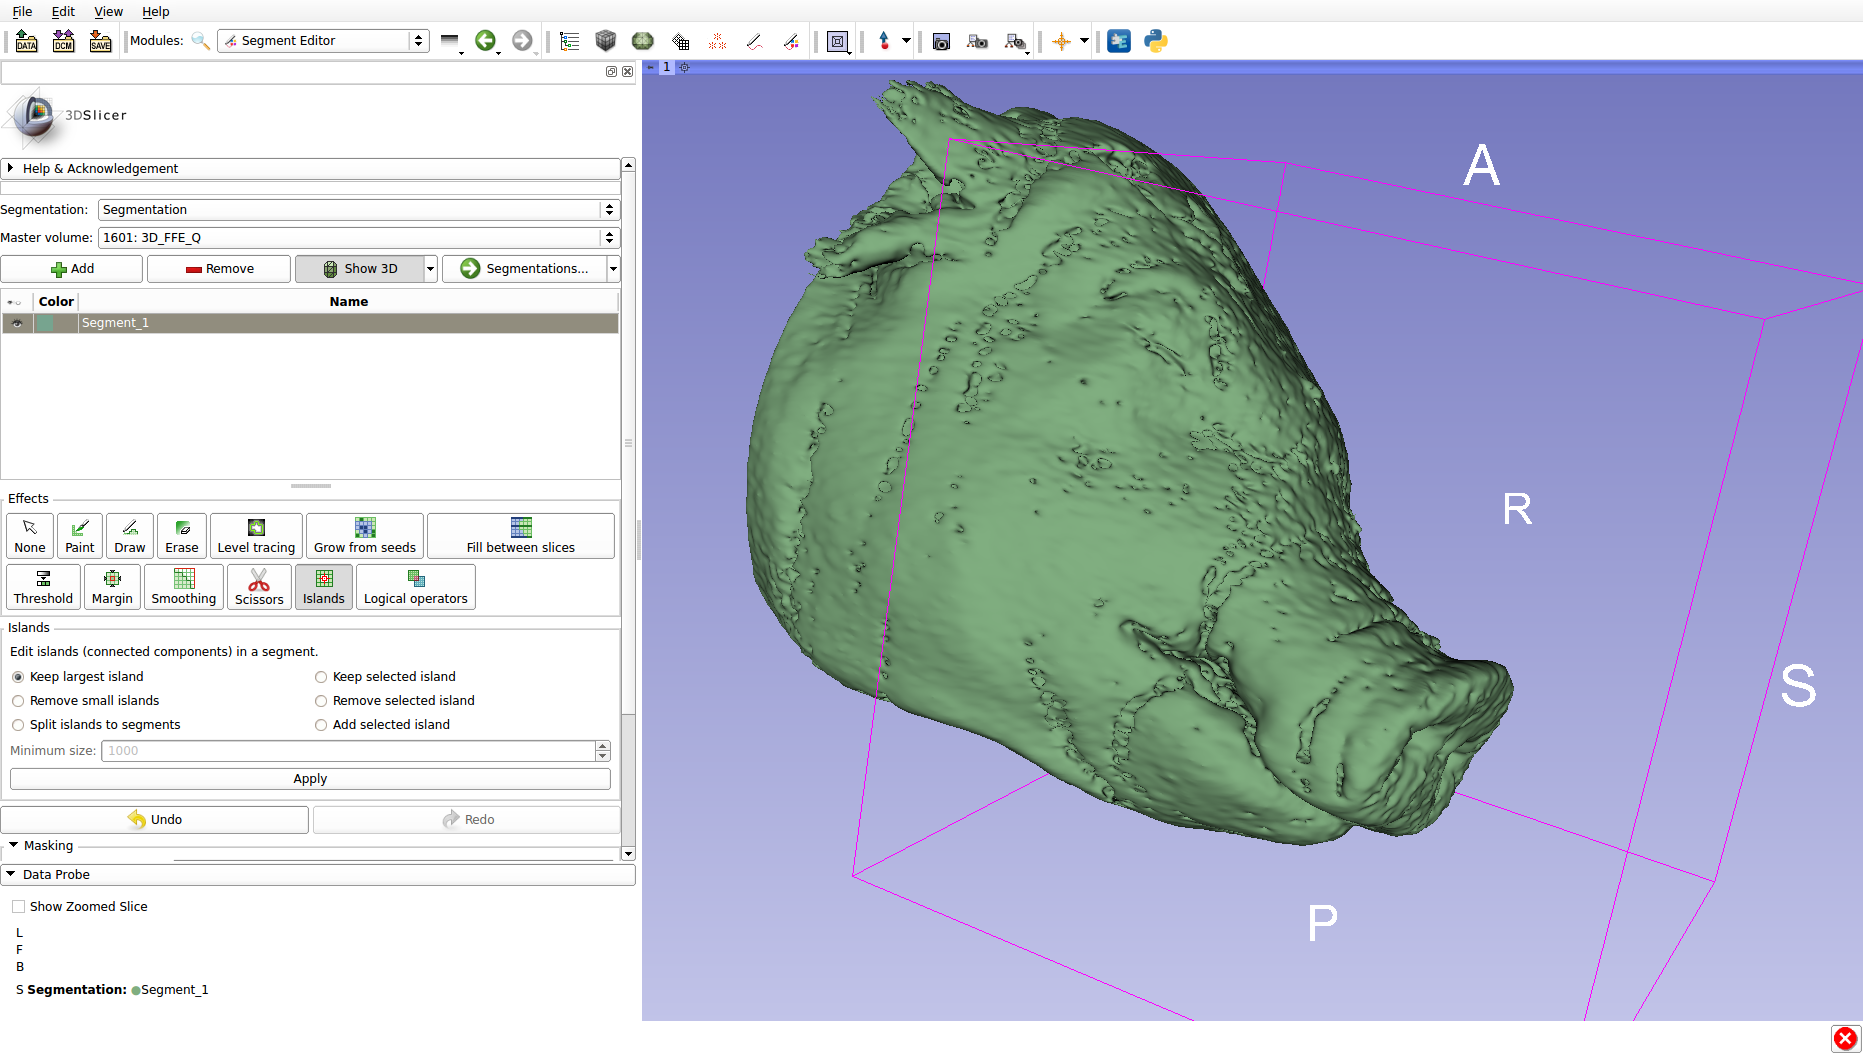
\includegraphics[width=\textwidth]{images/segmentation_islands.png}
    \caption{Screenshot of Slicer showing the rendered mesh of the patient head once islands were removed from the mask.}
    \label{fig:slicerHeadMeshNoFilter}
\end{figure}

To remove noise from the model and smooth the surface finish, two rounds of filters were used on the segment of the patient head. The first was a closing filter, which connected the mesh surface over holes under 3mm in diameter. This had the effect of also closing some internal geometry that added unnecessary polygon counts to the mesh, as seen in \autoref{fig:segmentationClosing}.

\begin{figure}[thpb]
	\centering
	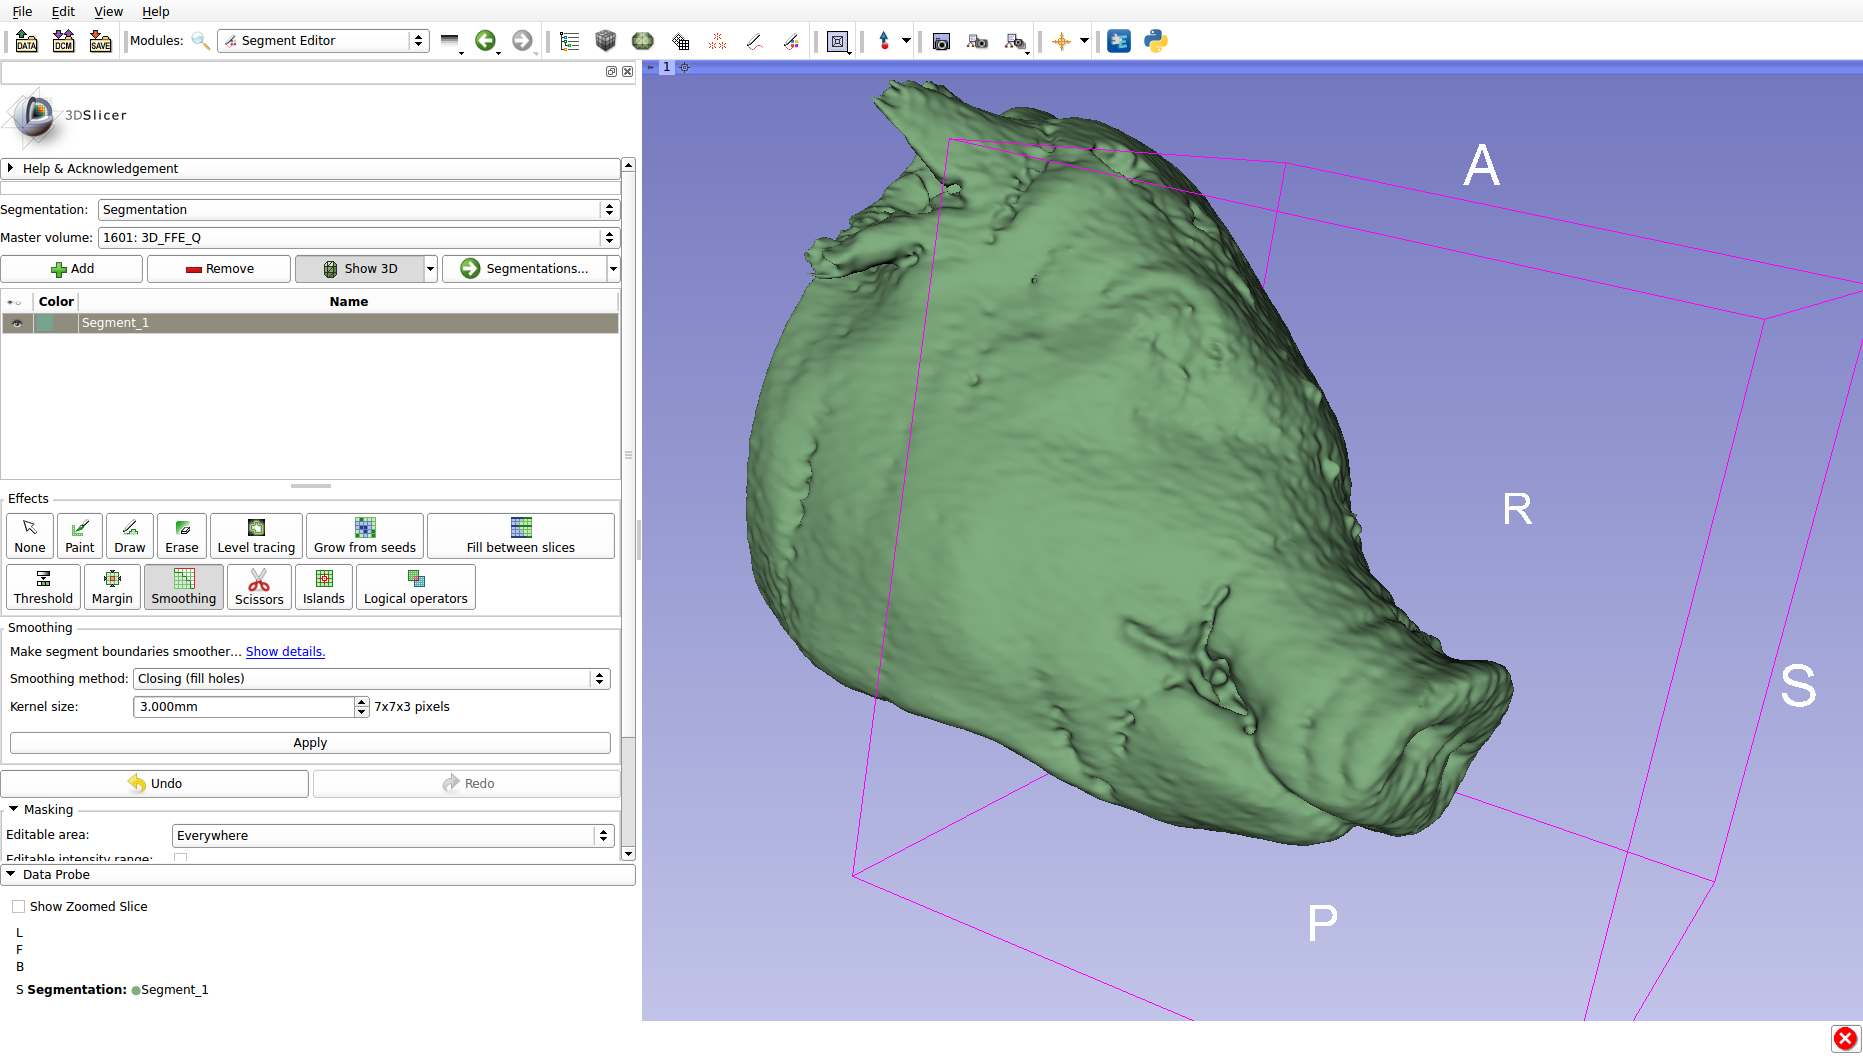
\includegraphics[width=\textwidth]{images/segmentation_closing.png}
    \caption{Screenshot of Slicer showing the rendered mesh of the patient head after a closing filter was applied.}
    \label{fig:segmentationClosing}
\end{figure}

Next, a normal filter with a setting of 4mm was used to generally smooth the model's surface. This would remove some of the detailed texture of the patient's head, but kept the geometric shape suitably. A rendering of the volume after the filtering is shown in \autoref{fig:slicerHeadMeshFiltered}. The segmentation was then exported as a model within Slicer through the segmentations module, which was the same format in which the workspace polydata objects were stored in. This model was then named patient head and sent over OpenIGTLink, which could take a couple dozen seconds to serialize, transmit, and deserialize on the receiving end due to the size of the polydata.

\begin{figure}[thpb]
	\centering
	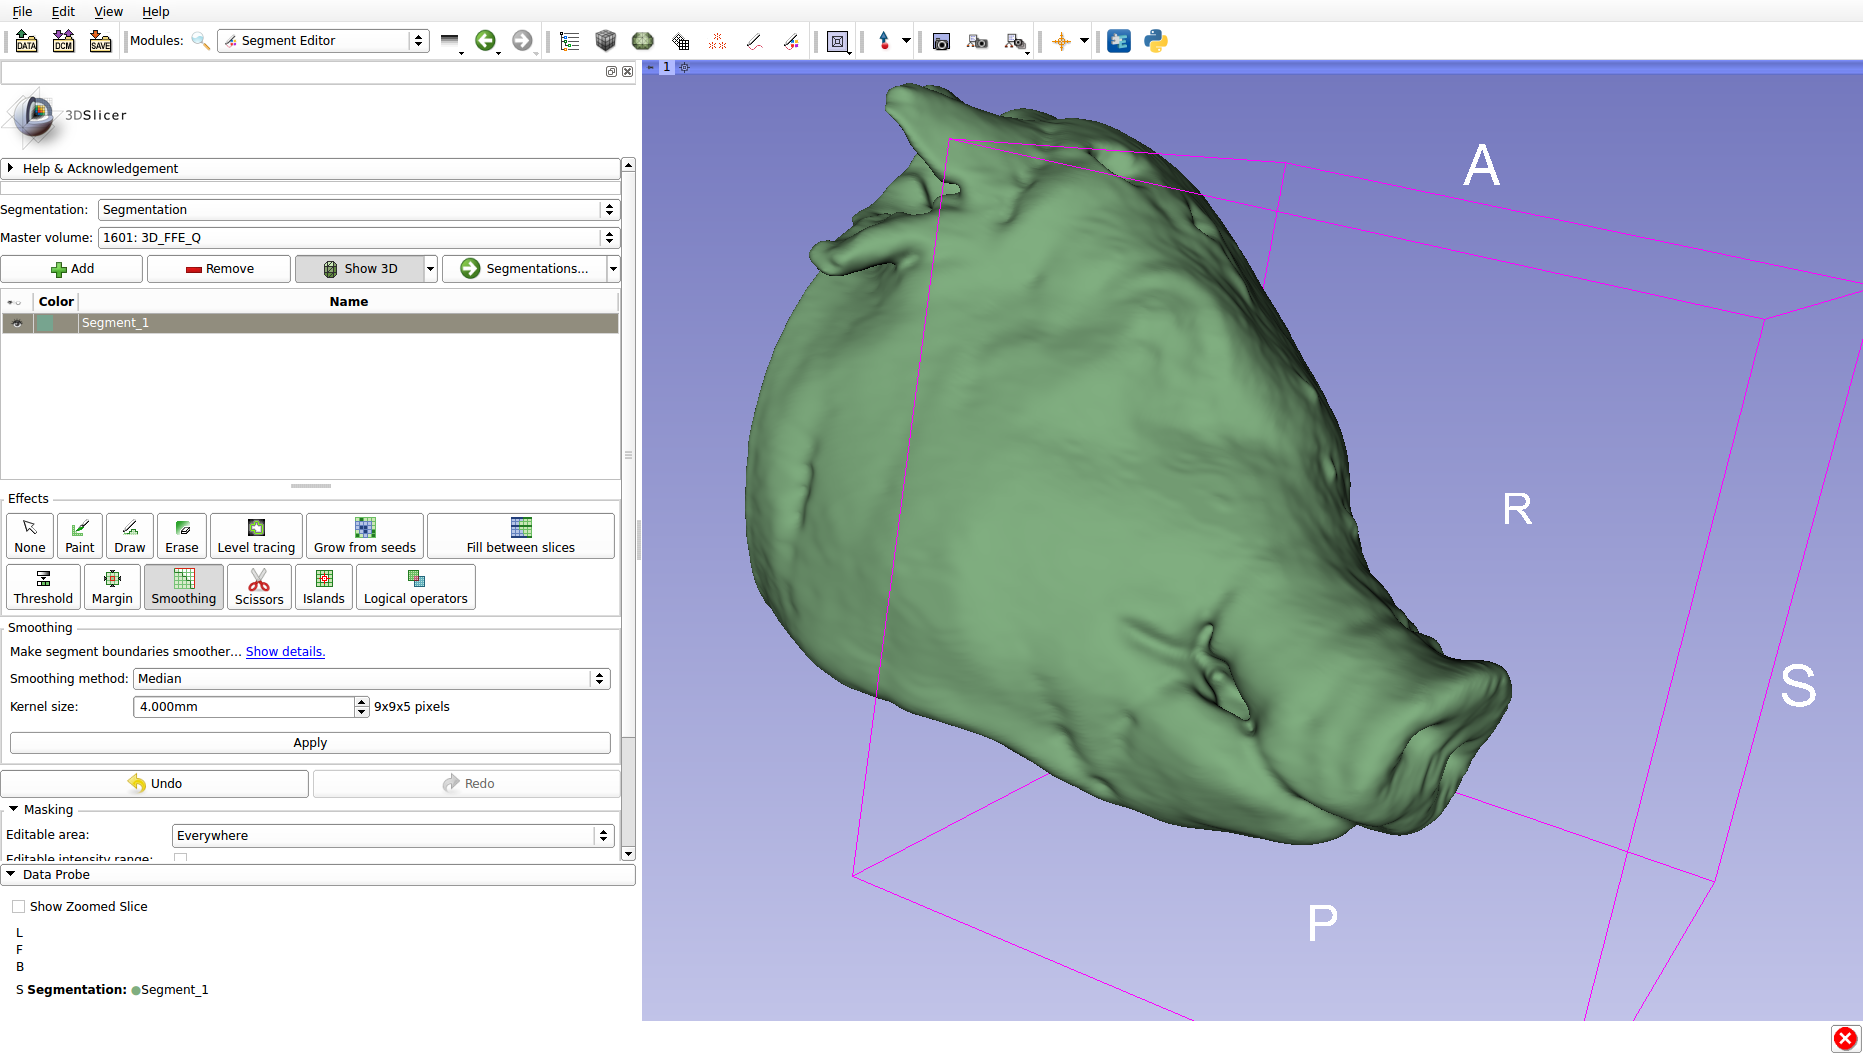
\includegraphics[width=\textwidth]{images/segmentation_smoothing.png}
    \caption{Screenshot of Slicer showing the rendered mesh of the patient head after normal filtering.}
    \label{fig:slicerHeadMeshFiltered}
\end{figure}


\section{ROS Processing}
Since collision checking is a time-consuming process, any method of simplifying the geometry of the collision objects can help reduce the processing time for motion planning. The fidelity of the meshes produced by the segmentation in Slicer was much higher than would be required for motion planning, so the triangle count of the polydata objects could be reduced to speed up collision checks. Ideally, collision meshes should simply be a solid shell as only the outer surface is necessary for checking against collisions. To quickly remove the internal geometry of the mesh, the same concave hull process for wrapping point clouds with meshes (as discussed in \autoref{sec:sendingWorkspaceVolume}) was used. This moved the rest of the processing to ROS, so the volume from the segmentation completed in Slicer was then sent over OpenIGTLink. 

A different ROS node was created with the same basic format as the point cloud converter, but in this case, it subscribed to the OpenIGTLink polydata topic and published to the planning scene monitor. Incoming polydata messages were converted to VTK types, then a decimation process was used to reduce the triangle count by 95\%. \autoref{fig:segmentationDecimated} shows what that decimated mesh looked like if it was viewed in Slicer.

\begin{figure}[thpb]
	\centering
	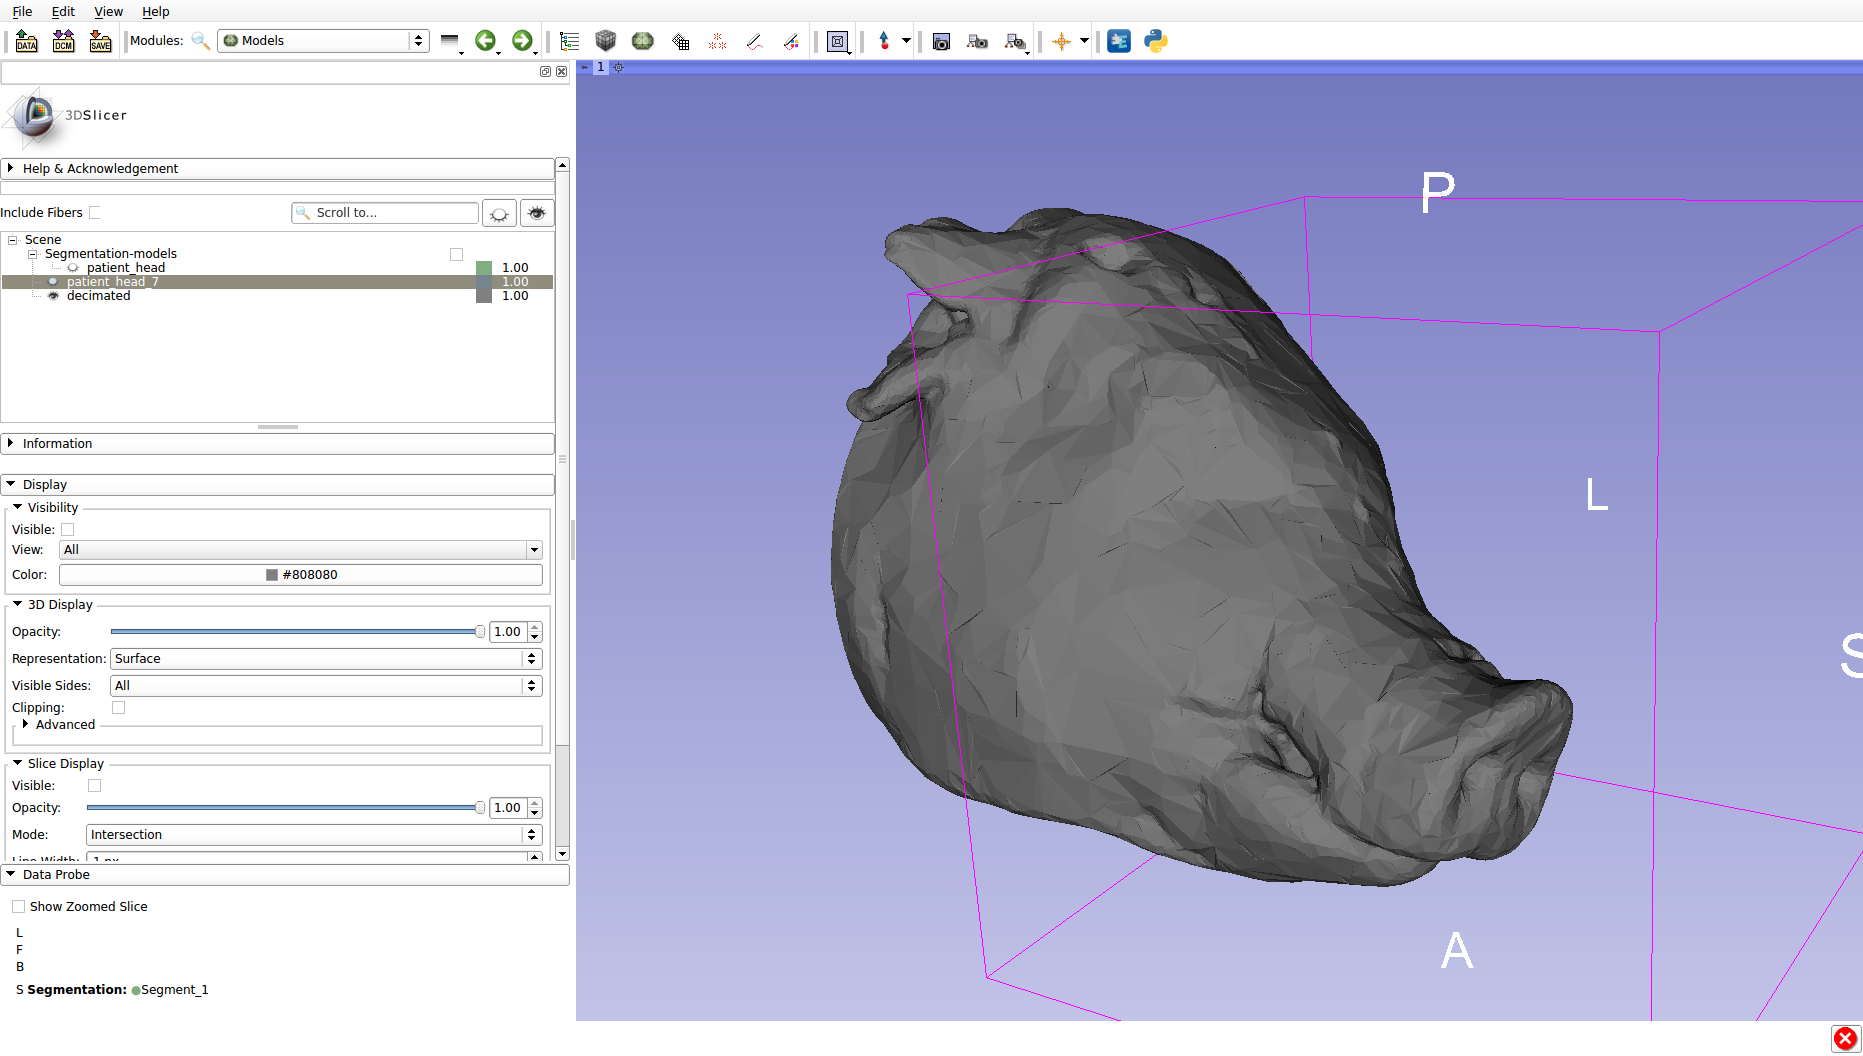
\includegraphics[width=\textwidth]{images/segmentation_decimated.png}
    \caption{Screenshot of Slicer showing the STL of the decimated patient head after processing from the ROS node.}
    \label{fig:segmentationDecimated}
\end{figure}

The decimated polydata object's points were \todo{GF:can you confirm that the low res head is not smaller that the high res one? It should ideally encompass the full high res one so it does not eliminate potential collisions.} converted to a PCL point cloud so the same code could be used for performing the concave hull approximation developed in \autoref{sec:sendingWorkspaceVolume}, and the resulting VTK object was saved to disk so that it could be viewed in Slicer for reference purposes, as shown in \autoref{fig:headMeshConcave}. The VTK object was then saved as an STL, and the STL path was published to the Workspace Visualizer so it could load the mesh resource as a collision object at the appropriate time and publish that to the planning scene. \autoref{fig:patientHeadInPlanningScene} shows the final outcome of this process with the patient head model properly loaded into the planning scene, attached to the base link of the robot to allow collision checks to be skipped for that link and to prevent false positives.

\begin{figure}[thpb]
	\centering
	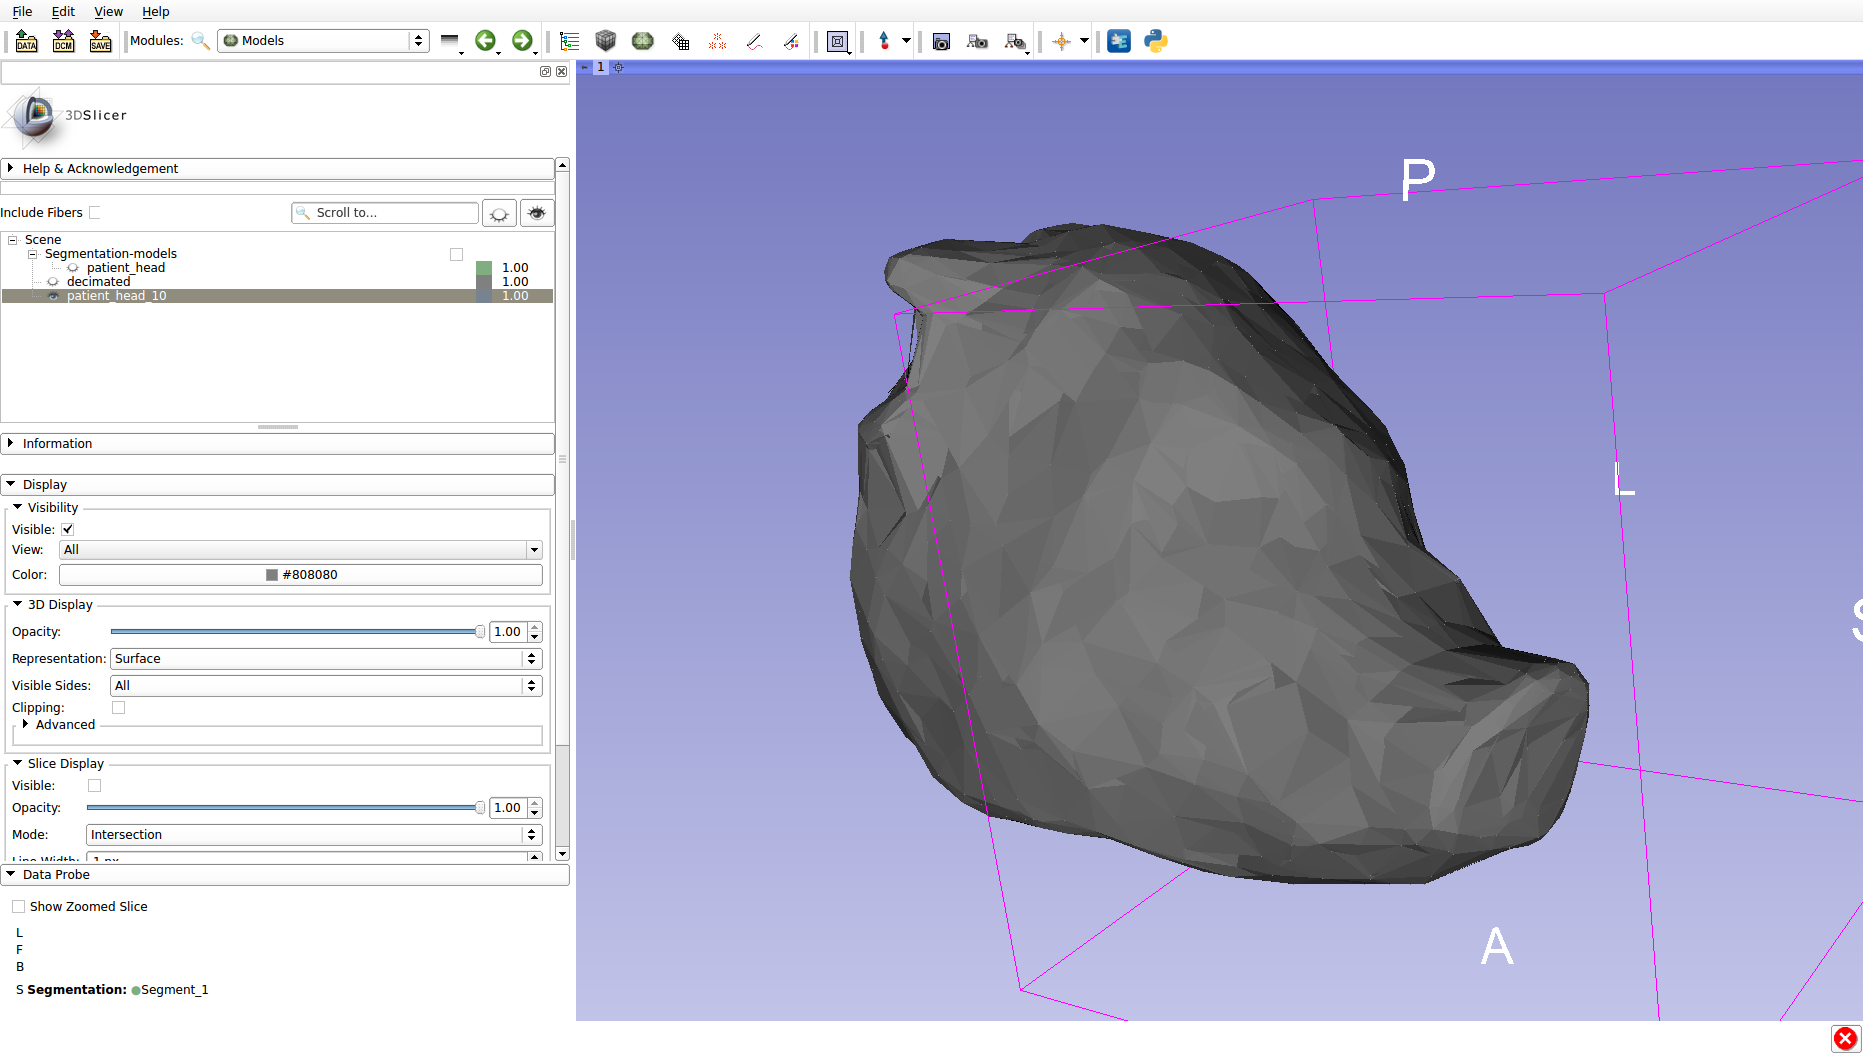
\includegraphics[width=\textwidth]{images/segmentation_convex_hull.png}
    \caption{The patient head shown in Slicer as a result of the concave hull operation.}
    \label{fig:headMeshConcave}
\end{figure}

\begin{figure}[thpb]
	\centering
	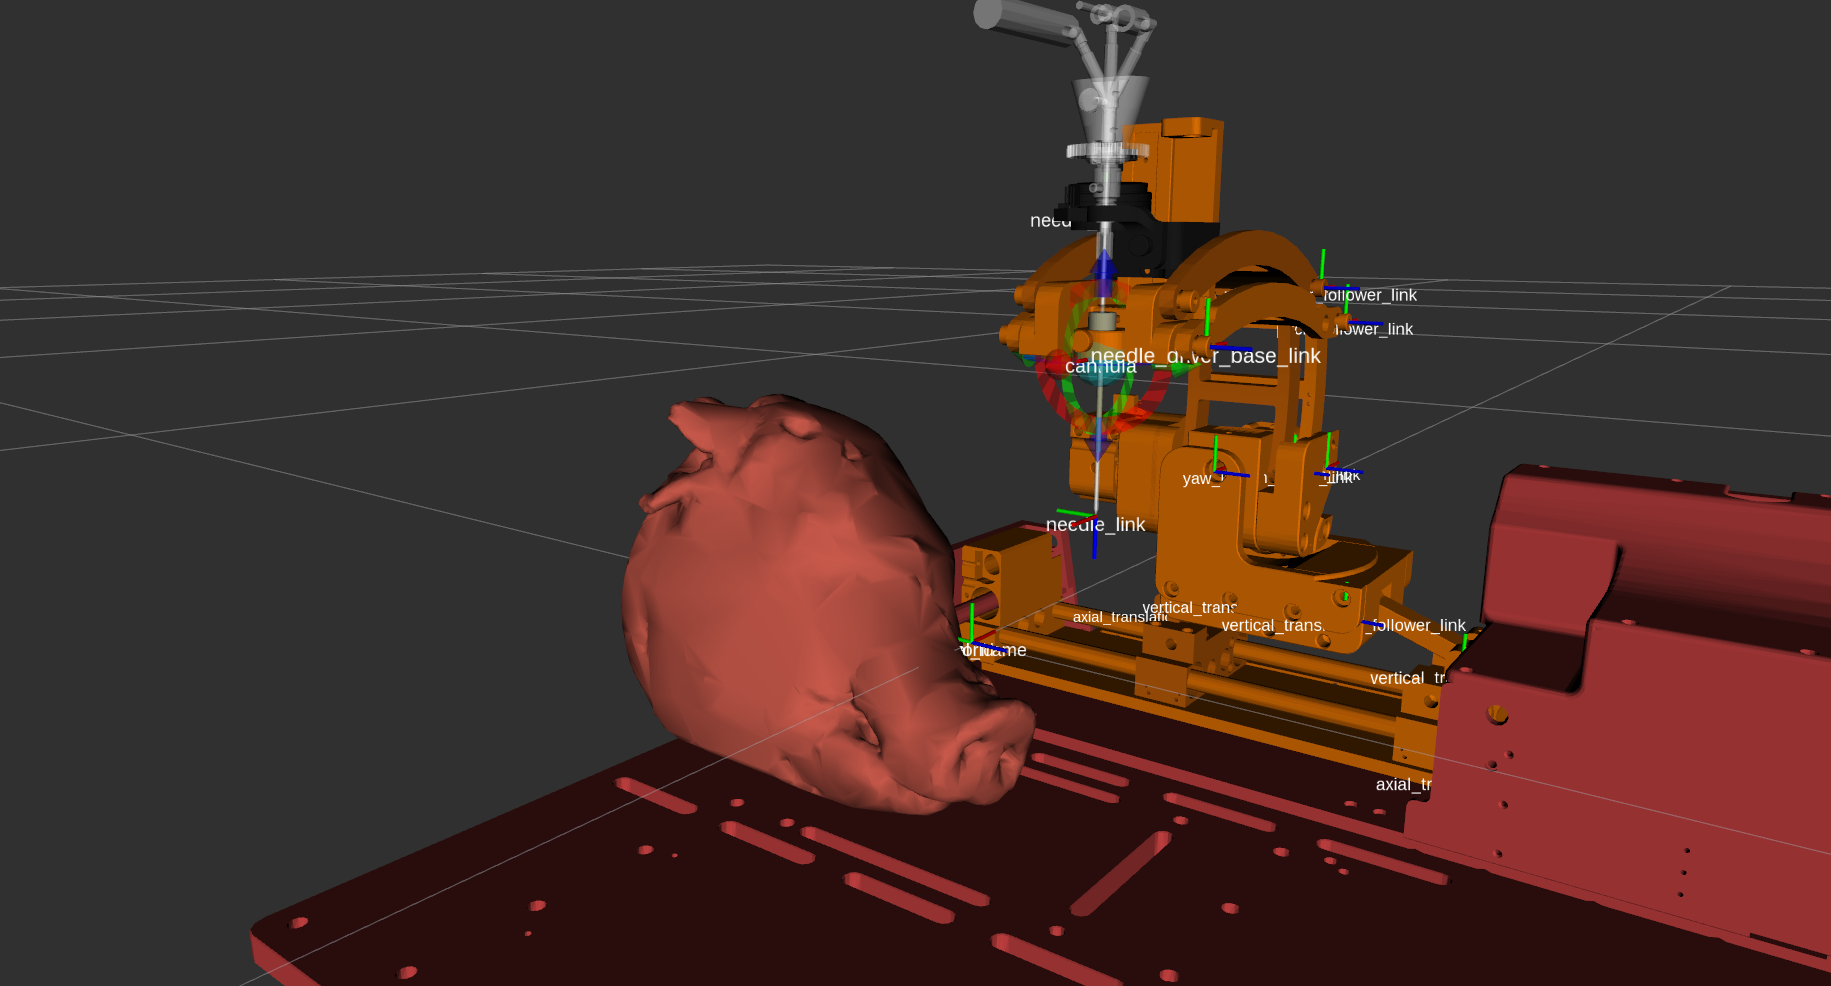
\includegraphics[width=\textwidth]{images/segmentation_rviz.png}
    \caption{The planning scene as shown in RViz with the patient head added as a collision object attached to the robot.}
    \label{fig:patientHeadInPlanningScene}
\end{figure}


%%%%%%%%%%%%%%%%%%%%%%%%%%%%%%%%%%%%%%%%%%%%%%%%%%%%%%%%%%%%%%%%%%%%%%%%%%%%%%%%
\chapter{Optimization of Patient Head Positioning}
\todo[inline]{Not sure this will happen. Revisit or move the below to future work. GF:what do you have in mind, and what is the status?}
An occasional problem that occurred during procedures was that in some cases, the patient's head or the burr hole was placed in way that was not conducive to the actual workspace of the neurobot. While the workspace visualization could show what was reachable on a trial and error process once the scans of the patient were taken, there would be great utility in a tool that could show optimal locations for the burr hole to be placed on the patient's skull given typical head orientations once the patient was in the scanner with the robot. Though an automated system which computes an optimal patient head orientation and burr hole based on MRI scans and pre-operative data would be desirable, sometimes a human can make equally valid decisions if they are provided with sufficient data in an easily understandable format.

% \section{Description of Optimization Problem}
% The patient head position and orientation could be optimized to provide the robot with greatest manipulability around the target area. This would involve consideration of the target area, typical burr hole locations on the skull, comfortable range of motion of the patient's head, and the flexibility of robot mounting locations. Though a challenging problem to solve, this could remove some of the uncertainty and replanning that occurs during procedures due to a patient position that prevents the robot from reaching the target site.
% \section{Implementation of Optimization Solution}


%%%%%%%%%%%%%%%%%%%%%%%%%%%%%%%%%%%%%%%%%%%%%%%%%%%%%%%%%%%%%%%%%%%%%%%%%%%%%%%%
\chapter{Experiments}
In order to validate that the system meets the user requirements and to better understand its performance and capabilities, several tests were completed. A series of metrics were collected for the IK solver and motion planning performance of the system. Then, tests were conducted using the actual robot to validate the workspace analysis and motion planning accuracy of the system, which inherently tests the modeling of the neurobot as well. 


\section{Benchmarking}
Several experiments were conducted in order to gain a better understanding of the execution time of the IK solver and the motion planning implementation. Tests were configured by determining a viable end effector needle pose by uniform random sampling from the configuration space of the robot and using the forward kinematics to compute the end effector position. This position was then fed back into the IK solver and the time it took the IK solver to compute the solution was measured. There were several variations of this test, with collision checking with the environment enabled and disabled for the motion planning section. Tests were conducted on a computer with a Ryzen 7 1700 processor operating at 3.00 GHz with 16GB of DDR4 RAM.

\subsection{IK Solver}
\todo[inline]{GF:how does this depend on configuration (start and end pose)? }
In the first experiment, the parameters of the IK solver, namely the number of allowed solver attempts and the allowed search time, were set at default values of 5 attempts and 0.01 seconds. \autoref{fig:ikTimeFixed} shows the execution time plotted over 200 iterations of the solver. Interestingly, the solving time was somewhat dependent on the order of the queries: the initial query takes the longest and the number of long queries decreases over time. This seemed to indicate a weak caching optimization to speed up processing. \todo{GF:these results are interesting. i guess not surprising since this robot does not really have singularities in the workspace. i assume would look very different for a generic 6-dof serial manipulator}

\begin{figure}[thpb]
	\centering
	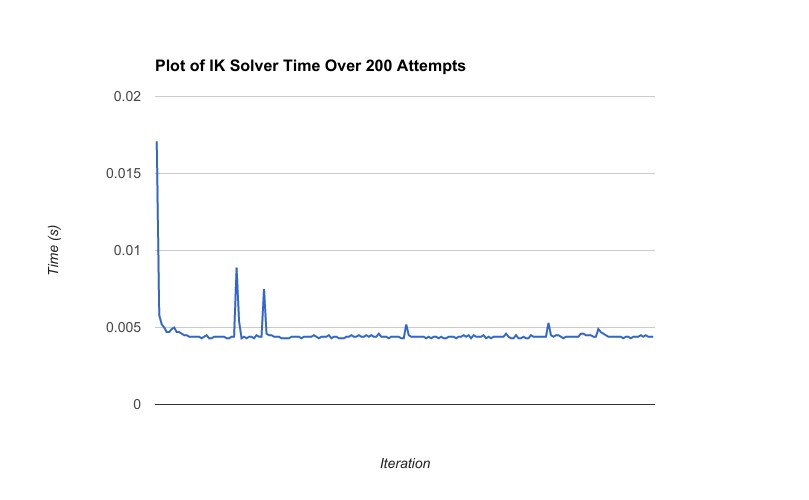
\includegraphics[width = 5in]{graphs/ik_solver_fixed_stats.png}
    \caption{Plot of inverse kinematics solver execution time to find viable joint configuration in collision free environment given a random reachable target over 200 consecutive trials. Average 0.004546s. 5 allowed attempts with 0.01s to find a solution.}
    \label{fig:ikTimeFixed}
\end{figure}

In the next experiment, the number of attempts was fixed at 1 and the time allowed for finding solutions was varied from 0.00001s to 0.00991s. \autoref{fig:ikexeTime} shows the results of the experiment. While a slight minimum appeared around 0.003s, there was not a strong trend, other than in longer search times, the execution time generally increased. \autoref{fig:ikHist} shows the same data but as a histogram plot. This seemed to indicate that providing longer search times did not have an impact on the execution time; solutions generally took around the same amount of time to converge.

\begin{figure}[thpb]
	\centering
	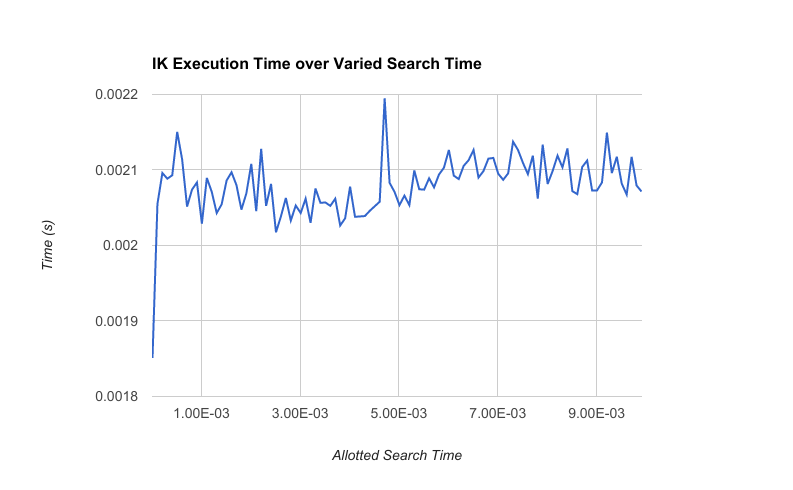
\includegraphics[width = 5in]{graphs/ik_exec_time_over_allowed.png}
    \caption{Plot of inverse kinematics solver execution time over allotted search time to find viable joint configuration in collision free environment given a random reachable target. 200 trials.}
    \label{fig:ikexeTime}
\end{figure}

\begin{figure}[thpb]
	\centering
	\includegraphics[width = 5in]{graphs/ik_hist_1_attempt.png}
    \caption{Histogram plot of inverse kinematics solver execution time to find viable joint configuration in collision free environment given a random reachable target. 200 trials. Average 0.00207957s}
    \label{fig:ikHist}
\end{figure}

In the final experiment with the IK solver, the number of attempts allotted to the solver was varied from 1 to 19, with 200 tests being conducted for each timing point. \autoref{fig:ikNumAttempts} shows the results of the test. Perhaps somewhat unsurprisingly, with only 1 attempt at solving the IK, the average execution time was highest since failure to find a solution would maximize the timeout allowed on the search without being able to spawn another search. Beyond 2 allowed attempts, there was no strong trend, indicating that the choice did not matter significantly.

\begin{figure}[thpb]
	\centering
	\includegraphics[width = 5in]{graphs/ik_sover_over_time.png}
    \caption{Plot of inverse kinematics solver execution time over number of allowed attempts to find viable joint configuration in collision free environment given a random reachable target. 200 trials averaged for each number of allowed attempts. Average 0.001707s}
    \label{fig:ikNumAttempts}
\end{figure}

\subsection{Motion Planner}
The motion planner was examined in the next set of experiments. Similarly to the tests for the IK solver, the same random valid configuration generation was used to set a desired pose to the needle planning group. In the first section, collisions with the environment were not considered, and in the final section, the patient head collision model was added to the environment and considered.

\subsubsection{Planning with No Patient Head}
\autoref{fig:plannerHist} indicates that most planning sessions lasted from 0.1s to 
0.225s, with a distribution tail towards longer execution times. However, no plans took longer than 0.5 second to generate, even given a limit of 5 seconds. This showed that motion plans without environment collision models to consider were fairly quick, but performance with environment collision checks could be significantly longer.

\begin{figure}[thpb]
	\centering
	\includegraphics[width = 5in]{graphs/planner_hist.png}
    \caption{Histogram plot of motion planner execution time to find path in collision free environment between 2 random configurations. 200 trials. Average 0.209805s}
    \label{fig:plannerHist}
\end{figure}

The path smoothing operation was also examined in some detail. \autoref{fig:pathHist} shows the execution time of the path smoothing algorithm, which indicated a relatively narrow distribution with a tail end towards longer execution times, similar to the distribution of planner times. This is expected as more complex trajectories take longer to generate and will also have a longer path, increasing the time it takes to adequately smooth it. In general, the path smoothing was a very small part of the total path planning operation.

\begin{figure}[thpb]
	\centering
	\includegraphics[width = 5in]{graphs/smoother_hist.png}
    \caption{Histogram plot of motion planner path smoothing execution time. 40 trials. Average 0.0000073s}
    \label{fig:pathHist}
\end{figure}

\subsubsection{Planning with Patient Head}
\todo[inline]{Complete these tests and write section.}


\section{System Workspace Validation}
\todo[inline]{GF:where are you at with these tests?}
To test the workspace validation, motion capture was used on the neurobot as it completed movements mimicing those generated during the workspace analysis on the modeled neurobot. The end goal was to directly compare the shape of the workspace obtained by the real hardware with that achieved by the software system. Fiducials were used on the robot's base to establish the base frame of the robot and a valid transform to directly relate the modeled robot frames with the simulated robot frames. A single fiducial was placed on the robot where the entry point would be located for the robot, as shown in \autoref{fig:workspaceExperimentSetup}.

\begin{figure}[thpb]
	\centering
	%\includegraphics[width=\textwidth]{diagrams/Software_Diagrams.pdf}
    \missingfigure[figwidth=4in]{picture of experiment.}
    \caption{Picture of the experimental setup of the neurobot for workspace validation.}
    \label{fig:workspaceExperimentSetup}
\end{figure}

a script commanded the robot to move to joint positions evenly spaced in the configuration space. Care on defining these points algorithmically was taken to ensure that the robot did not self-collide since the robot controller could not check for self collisions before executing a motion. Upon the completion of each movement, a control signal was sent to the motion capture signal to log the fiducial position before moving to the next point, eventually generating a point cloud of the entire workspace of the robot. These points were then parsed into a PCL point cloud and processed through the same mesh generation that the software system used for the simulated workspace. \autoref{fig:workspaceMocapCompare} shows an overlay of the real and simulated results of the entry workspace.

\begin{figure}[thpb]
	\centering
	%\includegraphics[width=\textwidth]{diagrams/Software_Diagrams.pdf}
    \missingfigure[figwidth=4in]{Overlay of entry workspace with simulated and actual results.}
    \caption{Entry workspaces compared between the real neurobot (color) and that computed by the workspace visualization system.}
    \label{fig:workspaceMocapCompare}
\end{figure}

\todo[inline]{Revisit for analysis once tests are complete.}


\section{Trajectory Validation}
To validate the trajectory generation and execution, a similar setup was used as in the previous section. For this test, a simple cube was placed in the actual robot's space and carefully measured from the base. A geometric cube of the same size was added to the robot in the same position in the planning scene within ROS. The fiducial remained on the entry point of the robot. \autoref{fig:trajectoryExperimentalSetup} shows the experimental configuration for this test.

\begin{figure}[thpb]
	\centering
	%\includegraphics[width=\textwidth]{diagrams/Software_Diagrams.pdf}
    \missingfigure[figwidth=4in]{picture of experiment.}
    \caption{Picture of the experimental setup of the neurobot for trajectory validation.}
    \label{fig:trajectoryExperimentalSetup}
\end{figure}

In the software system, a motion plan was requested to a goal which could result in a collision if the robot position was linearly interpolated to that point. Once the motion plan was computed and the trajectory of the entry point was saved, the real robot executed the same trajectory, triggering a frame capture at each point a segment in the trajectory was reached. The path of the actual robot was then saved as a point cloud and compared to the desired trajectory as determined by the motion planning software, as shown in \autoref{fig:trajectoryMocapCompare}.

\begin{figure}[thpb]
	\centering
	%\includegraphics[width=\textwidth]{diagrams/Software_Diagrams.pdf}
    \missingfigure[figwidth=4in]{Overlay of trajectory end effector path in RViz with simulated and actual results.}
    \caption{Trajectory path compared between the real neurobot (color) and that computed by the motion planning system.}
    \label{fig:trajectoryMocapCompare}
\end{figure}

\todo[inline]{Revisit for analysis once tests are complete.}

%\section{Patient Head Optimization Results}


%%%%%%%%%%%%%%%%%%%%%%%%%%%%%%%%%%%%%%%%%%%%%%%%%%%%%%%%%%%%%%%%%%%%%%%%%%%%%%%%
\chapter{Conclusions}
\todo[inline] {Discuss how this is a prototype and the tools worked, but something more suitable is needed.}
This project demonstrated the successful implementation of a system compatible \todo{GF:very nice, but maybe also a bullet list of key outcomes that models the one in the intro} with the medical platforms OpenIGTLink and Slicer, capable of generating the reachable workspace of the neurobot by checking for collisions with the scanner, and generating collision-free trajectories which yielded improvements to procedure time and understanding of the capabilities of the neuroablation robot platform. The system achieved its objectives, including interfacing with Slicer, assessing the robot workspace, generating motion plans to the entry point of the skull, creating a 3D volume of the patient's head suitable for collision detection, and providing a mechanism for assisting surgeons with planning procedures with the neurobot to best use its capabilities.  

The system design proved suitable for achieving the objectives at hand and maintaining a good level of modularity and maintainability. The software system was implemented successfully with special attention paid to interfaces between environments. The software distribution through a VM met requirements, but perhaps a less clunky solution would be to use a system such as Docker to avoid the less involved process of installing and maintaining a VM.

Modeling the robot in ROS was possible by decoupling the motions on the differential screw drive. While the URDF format did not offer a mechanism for modeling parallel robots directly, the system functioned adaquately, but with some added complexity of having to manage the entire robot state when planning for a single chain of joints. KDL does allow for solving parallel kinematic chains, but the ROS TF package cannot truly describe the kinematic state of such systems. \cite{kdl} There could be benefit to directly interfacing with KDL, yet the benefits of utilizing higher level features found in MoveIt! tended to offset drawbacks for this use case.

Workspace examination was a success, with the ability to see the entry workspace of the robot directly in Slicer overlaid on surgical images. The examination included consideration of the scanner bore as a collision object, which ensured that the outputted workspace would be accurate and prevent the possibility of finding a robot configuration that reached the target but collided with the bore. Providing the workspace given the entry point was very helpful in formulating a method for determining how flexible a chosen entry point was in allowing a greater number of treatment sites to be targeted and helping the surgeon realize the importance of locating the burr hole in a way to best utilize the ability of the neurobot.

The motion planning components functioned desirably in generating a trajectory which moved the robot to the entry point without colliding with the patient head, removing the cumbersome step in the procedure of moving the robot joint by joint to the correct configuration in order to avoid collisions. MoveIt! proved a reasonable platform for developing a `turn-key' motion planning system, yet it did mask several more advanced features of OMPL. For instance, cost functions could not be modified; they were locked to OMPL defaults by the MoveIt! interface. \cite{moveitIssue} To attain cost functionality adjustment, OMPL must be utilized directly without the MoveIt! wrapper. This would significantly increase development time, but could prove advantageous in other ways, allowing better tuned motion planning algorithms to be used to speed up planning time and potentially develop better paths. Yet with some of the shortcomings with MoveIt!, its ease of use and installation met the requirements set forward by the project and performed as necessary.

Working from MRI scans of the patient's head, the segmentation and extraction of the volume for use in collision detection proved adequate for accurately producing motion plans within a tightly constrained environment. The hand-off between Slicer and ROS yielded the best case of software reuse and utilized each systems' capabilities to the fullest. 

Results and testing show that the system performed the motion planning sufficiently quickly to be useful on the actual robot hardware. Trajectory generation to a valid pose consumed an average of 0.21 seconds with no collision objects, and as the motion of the robot to an entry point on the skull will generally be collision free, this approach promised to be significantly faster than manually planning and executing trajectories by driving the robot joint by joint in the operating room. Further experimentation showed that the actual neurobot produced a similar practical workspace, validating the modeling of the robot and the accuracy of the workspace generation using the tools supplied by ROS and MoveIt!. Finally, tests using motion capture demonstrated the system was capable of accurately tracking the generated trajectories and could avoid colliding with objects in the environment.

In the process of developing these capabilities for the system, there were some libraries and tools that could use some additional development that, if fixed, would make consequent developing on them easier and reduce the amount of work for bringing new systems online. To summarize, these were:
\begin{itemize}
\item ROS-OpenIGTLink-Bridge - including conversion nodes to only publish standard ROS messages outside the bridge package.
\item SolidWorks to URDF - saving joint limit configurations, improvements to auto-detection of joint type.
\item MoveIt! Planning Groups - better support for mimic joints.
\end{itemize}


%%%%%%%%%%%%%%%%%%%%%%%%%%%%%%%%%%%%%%%%%%%%%%%%%%%%%%%%%%%%%%%%%%%%%%%%%%%%%%%%
\chapter{Future Work}
While the system was successful in meeting its objectives and requirements, there were some improvements that could be made to further improve its capability and utility. Natural extensions to this project could benefit the greater community as a whole with sufficient resources and time.

As mentioned previously, utilizing the software within a VM was not an ideal design choice, but given the time constraints, requirements, and delicate nature of software environments and library installations, this was the best balance of performance and cost. With additional time, it would be ideal to contain the software with Docker or in some way integrate the system better to reduce this extra complexity. It could be possible to make a hardware change to solve this problem too. A high-performance traditional x86 processor in a small form factor (such as an Intel NUC) could be added to the neurobot control box or as the means of providing network communication over the fiber cable and hosting some other higher level functions. This would also yield the benefit of exposing the neurobot to the ROS environment, and perhaps tighter integration of the neurobot with ROS could spur some additional development or integration with other hardware platforms.

In modeling the neurobot, there were some changes that could be made to the SolidWorks to URDF add-in that could enhance its functionality, such as saving the joint configuration data and improving the joint type auto detection. While the workflow of updating a robot model and migrating those changes into URDF is not too burdensome, addressing these problems would greatly speed the process of completing those updates, as had to be done in this project. Eventually, building a simulation of the neurboot in ROS' simulation environment, Gazebo, could help fine-tune the neurobot controls and allow the motion planning solution to be more vested and allow proper unit testing, especially since it is possible in Gazebo to model parallelogram linkages. It would be interesting to develop a simulation of an MRI scanner as well and attempt to model the entire workflow. 

In the workspace analysis, the probe should be rotated during collision checks to make sure that a given configuration allows the probe to be rotated during treatment without hitting the MRI bore. This was not important during current testing of the neurobot since a symmetric probe was used during treatments, but more sophisticated treatments using a narrow beam probe would need this enhancement, albeit at a performance cost. The resolution of the workspace checking could also be enhanced, and perhaps an analytical workspace analysis would be worth developing to reduce the processing time. Alternatively, saving workspaces for the different probe configurations, effectively caching them and loading the proper configuration given the offset specifications, could massively reduce the computational time currently required for checking collisions with the bore and generating the workspace. 

Since a significant portion of this project involved developing a tool for completing the workspace analysis of the neurobot, it would be a valuable endeavor to make the solution more generic and release it as a freely available ROS package for conducting workspace analysis. This would take some additional development effort and a commitment from developers (or enough interest in the community) to continue supporting and updating the package as ROS continues to develop. Yet the effort would be worth it by helping WPI and AIM Lab become more public and well-recognized in the robotics community for their contributions.

In evaluating the validity of the planned trajectory in Slicer, it would be helpful to have a visualization of the robot and the ultrasonic probe that could be traced along the planned trajectory. This would provide a more thorough understanding of the positioning context of the system as it relates to the patient within the MRI machine as well as ensuring that parts of the robot would not strike the patient when executing the trajectory. There could have been more features added to the Slicer interface to better improve the interaction with the motion planning system, but further improvements were not possible in the given time frame.

The patient head pose and burr hole location could be algorithmically optimized (rather than through an operator-informed decision) to ensure maximum reachability around the tumor location by porting the robot model into OpenRave and utilizing existing optimality planners for determining where to locate the base of industrial robot manipulators. \cite{workspaceChecker} With the robot model properly represented in OpenRave, a functioning IKFast plugin could be created as well to enable analytical IK solving of the robot's end effector, which would improve the execution time when solving the IK during the entry point workspace checking.

\todo[inline]{Making the head segmentation more automated.}

\todo[inline]{Calibrating joint limits.}

\todo[inline]{GF:can we make the end effector a separate model w/ its own URDF that is imported into the arm URDF? Adnan/Radian/Ankur are doing similar w/ davinci to make the tool separate form the arm.}

More development support for the ROS-OpenIGTLink-Bridge package would open up the door for greater interoperability between the medical and robotics research worlds. However, there are some soul-seeking questions that need to be answered. How much reinventing happens on each side of the fence? There are excellent visualization tools for each platform, but it would be difficult to migrate features from one into another; perhaps there must always be two interfaces for interacting with medical data and robotics sensory information. Additionally, a lot of these tools are for research purposes only \todo{Flesh out how to turn this into a production system} and could be hard to attain Food and Drug Administration approval for human treatments due to validating operational safety on a large, open-source software stack and ensuring proper security protocols (to ensure patient privacy and safety) on both ROS and OpenIGTLink communications, not to mention potential licensing issues. Surpassing these more intricate issues can necessitate developing in-house solutions, which greatly increases cost and tends to result in reproducing solutions to basic problems that already exist. Perhaps there is a greater conversation that needs to happen in this front, but at the same time, it is sometimes better to prove out a system concept quickly with the best tools on hand rather than miss an opportunity for sake of technicality to offer a novel treatment system for treating clinical threats to human life and improving the quality of living for those suffering from neurological diseases.


%%%%%%%%%%%%%%%%%%%%%%%%%%%%%%%%%%%%%%%%%%%%%%%%%%%%%%%%%%%%%%%%%%%%%%%%%%%%%%%%
\appendix
\chapter{Multimedia Resources}
\label{sec:appendixVideos}
Videos of the system in operation are listed below: \todo{update with videos from presentation, add presentation link}
\begin{enumerate}
\item Robot and joint movements visualized in RViz \url{https://youtu.be/A8vxQcD-D1M}
\item MoveIt! Planning Scene with MRI Bore and head \url{https://youtu.be/uBkmzkpJ0bE}
\item Collision-aware IK in MoveIt! Scene \url{https://youtu.be/aWqPCrOiD8k}
\item Workspace checking demonstration \url{https://youtu.be/w9iJODJL3ho}
\item Trajectory planning demonstration with cannula \url{https://youtu.be/qjk9I6ZQJBc}
\item Trajectory movement with needle tip planning group \url{https://youtu.be/b-VsMk519GQ}
\end{enumerate}


\chapter{User Documentation}
\label{sec:userDocumentation}
\todo[inline]{add docs once finalized.GF: very important!}

\todo[inline]{GF:can you please be very clear, perhaps a bullet list, of specifically what needs to be updated after regenerating so that we can readily do it after modifications to the robot design ideally step by step instructions on what to do after design updates, could be in user guide}

\chapter{Technical Documentation}
\label{sec:technicalDocumentation}
\todo[inline]{Add docs once finalized.}

\section{OMPL Windows Installation}
\label{sec:omplWindowsInstallation}
This section includes some of the information found and steps for installing OMPL on Windows, which was eventually abandoned in favor of utilizing the OMPL installation included in ROS MoveIt!. It is included here as a reference for other individuals who may wish to continue these efforts.

\singlespacing
Install OMPL on Windows:
\begin{itemize}
\item \url{http://ompl.kavrakilab.org/installation.html}
\item \url{https://bitbucket.org/ompl/ompl}
\item \url{https://searchcode.com/file/102912958/doc/dox/installation.md}
\item \url{https://cmake.org/download/}
\item \url{https://bitbucket.org/ompl/ompl/src/tip/.appveyor.yml?fileviewer=file-view-default}
\end{itemize}

Install python 2.7:
Make sure to select to add python to system path

Install these things: \url{http://pygccxml.readthedocs.io/en/develop/install.html}
\begin{lstlisting}
pip install pygccxml
\end{lstlisting}
Install py++ \url{http://pyplusplus.readthedocs.io/en/latest/download.html}

CMAKE:
\url{https://cmake.org/download/}

Add to system path in install options

MinGW: \url{http://www.mingw.org/}
Click download \url{http://www.mingw.org/download/installer?}

MinGW wiki: \url{http://www.mingw.org/wiki/Getting_Started/}
\begin{lstlisting}
 $env:Path += ";D:\MinGW\bin"
cmake -G "MinGW Makefiles" ../.. [-DCMAKE_INSTALL_PREFIX=../../..]
cmake -G "MinGW Makefiles" ../..
\end{lstlisting}
Note: cannot have AVR installed on the same machine...

\url{https://andres.jaimes.net/718/how-to-install-the-c-boost-libraries-on-windows/}

Download and install boost for Windows: \url{https://dl.bintray.com/boostorg/release/1.65.0/binaries/}

Need 1.64 \url{https://sourceforge.net/projects/boost/files/boost-binaries/1.64.0/}

Do:
\begin{lstlisting}
$env:Path += ";D:\MinGW\bin"
Cd into the directory
.\bootstrap.bat gcc
.\b2.exe install --prefix=d:/boost_install toolset=gcc

b2 install --prefix=c:/installation/path toolset=gcc

$env:BOOST_ROOT = "D:\boost_1_64_install\"
$env:BOOST_LIBRARYDIR = "D:\boost_1_64_install\lib"
$env:BOOST_INCLUDEDIR = "D:\boost_1_64_install\include"
\end{lstlisting}

\url{https://stackoverflow.com/questions/20969280/find-package-doesnt-detect-boost-on-windows-cmake}
\url{https://stackoverflow.com/questions/19303430/cmake-cannot-find-boost-libraries}
\url{https://andres.jaimes.net/718/how-to-install-the-c-boost-libraries-on-windows/}


Apparently, boost is always built on a CMake version that is in the development pipeline... \url{https://github.com/Kitware/CMake/commit/fa114e7d708b76f33878f6f82a6c2a2e50c1c10f} So have to reinstall an older version of boost or build CMake from source.

\url{https://stackoverflow.com/questions/42123509/cmake-finds-boost-but-the-imported-targets-not-available-for-boost-version}

Install \url{https://tortoisehg.bitbucket.io/} to pull and build Cmake from source...



%%%%%%%%%%%%%%%%%%%%%%%%%%%%%%%%%%%%%%%%%%%%%%%%%%%%%%%%%%%%%%%%%%%%%%%%%%%%%%%%
% you can save some space by having the bibliography singlespaced, if you want
\singlespacing
\cleardoublepage

%
% You should become familiar with the BibTeX program, which
% uses a *.bib-file to collect all citations that you have. It's a lot
% prettier than typing all the citations right into the document. The 
% reference to citations also works well that way, but the exact 
% explanation of that will be on the CS-GSO homepage, whenever I'll ever 
% have time for that.
%
%
% If you use BibTeX, the bibliography is very easy. You refer to
% citations in the text with \cite{tag}, where tag is the tag that you
% defined in the bib-file.
% Then, you run bibtex once in a while during compilation, and the
% rest is done in two lines:
\begin{thebibliography}{99}

\bibitem{minimallyInvasiveSurgeryBenefits} Mohiuddin, Kamran, and Scott J. Swanson. ``Maximizing the benefit of minimally invasive surgery.'' Journal of surgical oncology 108.5 (2013): 315-319.

\bibitem{broadPerspectivesMinimallyInvasiveSurgery} Dimick JB, Ryan AM. ``Taking a Broader Perspective on the Benefits of Minimally Invasive Surgery.'' JAMA Surg. 2013;148(7):648. \url{https://doi.org/10.1001/jamasurg.2013.160}

\bibitem{daVinciEfficacy} Maeso, Sergio, et al. ``Efficacy of the Da Vinci surgical system in abdominal surgery compared with that of laparoscopy: a systematic review and meta-analysis.'' (2010): 254-262.

\bibitem{thermalAblation} Heather Webb, Meghan G. Lubner, J. Louis Hinshaw. ``Thermal Ablation,'' Seminars in Roentgenology. Volume 46, Issue 2, 2011. Pages 133-141. ISSN 0037-198X. \url{https://doi.org/10.1053/j.ro.2010.08.002}

\bibitem{thermalMRIAblation} Coluccia, Daniel, et al. ``First noninvasive thermal ablation of a brain tumor with MR-guided focused ultrasound.'' Journal of therapeutic ultrasound 2.1 (2014): 17. \url{https://jtultrasound.biomedcentral.com/articles/10.1186/2050-5736-2-17}

\bibitem{interstitialAblation} MacDonell J, Patel N, Rubino S, Goshal G, Fischer GS, Burdette EC, Hwang R, Pilitsis JG, ``Magnetic Resonance-guided Interstitial High-intensity Focused Ultrasound for Brain Tumor Ablation,'' Journal of Neurosurgery (JNS) Neurosurgical Focus, Vol 44, No 2, pp E11, Feb 2018. JNS, PubMed.

\bibitem{catheterAblation} Ghoshal G, Gee L, Heffter T, Williams E, Bromfield C, Rund L, Ehrhardt JM, Diederich CJ, Fischer GS, Pilitsis JG, Burdette EC, ``A Minimally Invasive Catheter-based Ultrasound Technology for Therapeutic Interventions in Brain: Initial Preclinical Studies,'' Journal of Neurosurgery (JNS) Neurosurgical Focus, Vol 44, No 2, pp E13, Feb 2018. JNS, PubMed.

\bibitem{texasOncology} Texas Oncology. ``Brain Tumor Surgery.'' Accessed 2017. \url{http://www.texasoncology.com/types-of-cancer/brain-cancer/surgery-for-brain-tumors}

\bibitem{openMRI} S. P. DiMaio and S. Pieper and K. Chinzei and N. Hata and S. J. Haker and D. F. Kacher and G. Fichtinger and C. M. Tempany and R. Kikinis. ``Robot-assisted needle placement in open MRI: System architecture, integration and validation.'' Computer Aided Surgery, 12(1), Pages 15-24. 2007. Taylor \& Francis. \url{https://doi.org/10.3109/10929080601168254}

\bibitem{stereotactic} Elekta. ``Lesell Stereotactic System.'' \url{https://www.elekta.com/neurosurgery/leksell-stereotactic-system.html}

\bibitem{aimLabRobot} Li G, Su H, Cole GA, Shang W, Harrington K, Camilo A, Pilitsis JG, Fischer GS, ``Robotic System for MRI-Guided Stereotactic Neurosurgery,'' IEEE Transactions on Biomedical Engineering, Vol 64, No 4, pp 1088-1088, April 2015. \href{http://aimlab.wpi.edu/includes/publications/2014_TBME_Li_Fischer_RoboticSystemforMRIGuidedStereotacticNeurosurgery.pdf}{Link}

\bibitem{neurobotIros} Nycz CJ, Gondokaryono R, Carvalho P, Patel N, Wartenberg M, Pilitsis JG, Fischer GS, ``Mechanical Validation of an MRI Compatible Stereotactic Neurosurgery Robot in Preparation for Pre-Clinical Trials,'' IEEE/RSJ International Conference on Intelligent Robots and Systems - IROS 2017, Vancouver, BC, Canada, Sept 2017. IEEE

\bibitem{needleSteeringSoftTissues} S. P. DiMaio and S. E. Salcudean, ``Needle steering and motion planning in soft tissues,'' in IEEE Transactions on Biomedical Engineering, vol. 52, no. 6, pp. 965-974, June 2005. doi: 10.1109/TBME.2005.846734

\bibitem{taskSpacePlanning} Greigarn, Tipakorn, and M. Cenk ??avu??o??lu. ``Task-space motion planning of MRI-actuated catheters for catheter ablation of atrial fibrillation.'' Intelligent Robots and Systems (IROS 2014), 2014 IEEE/RSJ International Conference on. IEEE, 2014.

\bibitem{prostateWorkspaceDesignAnalysis} Song, Sang???Eun, et al. ``A workspace???orientated needle???guiding robot for 3T MRI???guided transperineal prostate intervention: evaluation of in???bore workspace and MRI compatibility.'' The International Journal of Medical Robotics and Computer Assisted Surgery 9.1 (2013): 67-74.

\bibitem{workspaceOptimization} Hong Zaidi, Yun Chao, Zhao Lei and Wang Yang, ``A MRI-guided robot for neurosurgery: Optimization, registration and tracking,'' 2008 Chinese Control and Decision Conference, Yantai, Shandong, 2008, pp. 2222-2227. doi: 10.1109/CCDC.2008.4597718

\bibitem{thermalAblationFocusedUltrasound} ``Thermal Ablation'' Focused Ultrasound Foundation. \url{https://www.fusfoundation.org/mechanisms-of-action/thermal-ablation}.

\bibitem{hifu} Kennedy, James E. ``High-intensity focused ultrasound in the treatment of solid tumours.'' Nature reviews cancer 5.4 (2005): 321.

\bibitem{mri} ``Magnetic Resonance Imaging (MRI).'' National Institute of Biomedical Imaging and Bioengineering, U.S. Department of Health and Human Services, 2 Feb. 2017, \url{www.nibib.nih.gov/science-education/science-topics/magnetic-resonance-imaging-mri}.

\bibitem{mriSize} Jackson, Whitney L. ``MRI Machines Becoming More Patient-Friendly.'' Diagnostic Imaging, Modern Medicine Network, 12 Sept. 2011, \url{www.diagnosticimaging.com/mri/mri-machines-becoming-more-patient-friendly}.

\bibitem{isoStandardMRI} ``ISO/TS 10974:2012(En).'' Online Browsing Platform (OBP), ISO - International Organization for Standardization, 2012, \url{www.iso.org/obp/ui/#iso:std:iso:ts:10974:ed-1:v1:en}.

\bibitem{mriFrames} ``Coordinate Systems.'' Slicer Wiki, 30 June 2014, \url{www.slicer.org/wiki/Coordinate_systems}.

\bibitem{mrti} Stauffer, P. R., et al. ``Clinical utility of magnetic resonance thermal imaging (MRTI) for realtime guidance of deep hyperthermia.'' Energy-based Treatment of Tissue and Assessment V. Vol. 7181. International Society for Optics and Photonics, 2009.

\bibitem{mrtiAblation} Xiaonan R. Sun, PhD  Nitesh V. Patel, MD  Shabbar F. Danish, MD. ``Tissue Ablation Dynamics During Magnetic Resonance???Guided, Laser-Induced Thermal Therapy.'' Neurosurgery, Volume 77, Issue 1, 1 July 2015, Pages 51???58, https://doi-org.ezproxy.wpi.edu/10.1227/NEU.0000000000000732

\bibitem{openIGTLinkPaper} Tokuda, Junichi, et al. ``OpenIGTLink: an open network protocol for image???guided therapy environment.'' The International Journal of Medical Robotics and Computer Assisted Surgery 5.4 (2009): 423-434. \url{https://onlinelibrary.wiley.com/doi/full/10.1002/rcs.274}

\bibitem{openIGTLink} ``About OpenIGTLink.'' The OpenIGTLink Community and Brigham and Women's Hospital. 2018. \url{http://openigtlink.org/about.html}.

\bibitem{3DSlicerPaper} S. Pieper, M. Halle and R. Kikinis, ``3D Slicer,'' 2004 2nd IEEE International Symposium on Biomedical Imaging: Nano to Macro (IEEE Cat No. 04EX821), 2004, pp. 632-635 Vol. 1. doi: 10.1109/ISBI.2004.1398617 \url{http://ieeexplore.ieee.org/stamp/stamp.jsp?tp=&arnumber=1398617&isnumber=30417}

\bibitem{3DSlicer} ``3D Slicer.'' Brigham and Women's Hospital and 3D Slicer contributors. 2018. \url{https://www.slicer.org/}.

\bibitem{piezoLegs} Micromo. ``Piezo Motors Power MRI Robot.'' Micromo, a Member of the Faulhaber Group.  \url{https://www.micromo.com/applications/medical-lab-automation-equipment/piezo-motors-power-mri-robot}

\bibitem{neurobotIEEE2015} Li G, Su H, Cole GA, Shang W, Harrington K, Camilo A, Pilitsis JG, Fischer GS, ``Robotic System for MRI-Guided Stereotactic Neurosurgery,'' IEEE Transactions on Biomedical Engineering, Vol 64, No 4, pp 1088-1088, April 2015. \url{http://ieeexplore.ieee.org/xpl/articleDetails.jsp?arnumber=6945849}

\bibitem{zFrame} Shang W, Fischer GS, ``A High Accuracy Multi-image Registration Method for Tracking MRI-guided robots,'' SPIE Medical Imaging, San Diego, USA, Feb. 2012.

\bibitem{rosPaper} Quigley, Morgan, et al. ``ROS: an open-source Robot Operating System.'' ICRA workshop on open source software. Vol. 3. No. 3.2. 2009.

\bibitem{urdfExporter} Brawner, Stephen. ``SolidWorks to URDF Exporter'' ROS Wiki. 2017. \url{http://wiki.ros.org/sw_urdf_exporter}

\bibitem{rosOpenIGTLinkBridge} Frank T, Krieger A, Leonard S, Patel NA, Tokuda J, ``ROS-IGTL-Bridge: An Open Network Interface for Image-guided Therapy using the ROS Environment,'' International Journal of Computer Assisted Radiology and Surgery, May 2017. Springer.

% desire: include uncertainty rrt thing
\bibitem{planningAlgorithms} LaValle, Steven M. ``Planning algorithms.'' Cambridge university press, 2006. \url{http://citeseerx.ist.psu.edu/viewdoc/download?doi=10.1.1.225.1874&rep=rep1&type=pdf}

\bibitem{rrtStar} Karaman, Sertac, and Emilio Frazzoli. ``Sampling-based algorithms for optimal motion planning.'' The international journal of robotics research 30.7 (2011): 846-894. \url{http://citeseerx.ist.psu.edu/viewdoc/download?doi=10.1.1.419.5503&rep=rep1&type=pdf}

\bibitem{workspaceBiasing} Zucker, Matt, James Kuffner, and J. Andrew Bagnell. ``Adaptive workspace biasing for sampling-based planners.'' Robotics and Automation, 2008. ICRA 2008. IEEE International Conference on. IEEE, 2008. \url{http://www.ri.cmu.edu/pub_files/pub4/zucker_matthew_2008_1/zucker_matthew_2008_1.pdf}

\bibitem{kpiece} Sucan, Ioan A., and Lydia E. Kavraki. ``Kinodynamic motion planning by interior-exterior cell exploration.'' Algorithmic Foundation of Robotics VIII. Springer Berlin Heidelberg, 2009. 449-464. \url{http://www.wafr.org/wafr2008/papers/wafr08-sucan.pdf}

\bibitem{omplBenchmarks} Moll, Mark, Ioan A. Sucan, and Lydia E. Kavraki. ``An extensible benchmarking infrastructure for motion planning algorithms.'' arXiv preprint arXiv:1412.6673 (2014). \url{https://arxiv.org/pdf/1412.6673.pdf}

\bibitem{ompl} Sucan, Ioan A., Mark Moll, and Lydia E. Kavraki. ``The open motion planning library.'' IEEE Robotics \& Automation Magazine 19.4 (2012): 72-82. \url{http://ieeexplore.ieee.org/abstract/document/6377468/}

\bibitem{moveIt} Sucan, I. A., and Chitta, S. (2013). ``Moveit!.'' \url{http://moveit.ros.org.}

\bibitem{orocosKDL} Bruyninckx, Herman. ``OROCOS: design and implementation of a robot control software framework.'' Proceedings of IEEE International Conference on Robotics and Automation. 2002. \url{http://citeseerx.ist.psu.edu/viewdoc/download?doi=10.1.1.415.9503&rep=rep1&type=pdf}

\bibitem{openRave} Diankov, Rosen, and James Kuffner. ``Openrave: A planning architecture for autonomous robotics.'' Robotics Institute, Pittsburgh, PA, Tech. Rep. CMU-RI-TR-08-34 79 (2008).

\bibitem{ikFast} Diankov, Rosen. ``Ikfast: The robot kinematics compiler.'' 2010.

\bibitem{ikFastMoveIt} Sucan, I. A., and Chitta, S. (2016). ``Moveit! IKFast Plugin Tutorial.'' \url{http://docs.ros.org/kinetic/api/moveit_tutorials/html/doc/ikfast_tutorial.html}

\bibitem{moveitIssue} Sucan, I. A., and Chitta, S. (2013). ``ros-planning moveit issue 118'' \url{https://github.com/ros-planning/moveit/issues/118}

\bibitem{workspaceChecker} ROS.org ``reuleaux package documentation.'' Accessed April 2017. \url{http://wiki.ros.org/reuleaux}

\bibitem{kdl} Orocos Kinematics and Dynamics. ``KDL Wiki.'' Accessed April 2017. \url{http://www.orocos.org/kdl}

\end{thebibliography}

% \bibliographystyle{alpha}
% \bibliography{foo}

% which assumes a file foo.bib in your working directory.
% The word ``Bibliography'' will appear in your document as soon as
% you used ``bibtex'' on the command line.
%
% For reference on this, refer to the CS-GSO homepage.

%============================
%That's all, folks. Have fun.
%
%                     Andreas
%============================


\end{document}


% % Since this is a ``report'', the topmost level of hierarchy is
% % ``Chapter'', not section as you may be used to. Chapters are
% % enumerated starting from 1, so Sections are 1.1, Subsections are
% % 1.1.1, subsubsections don't get numbers. (You can change that, if
% % you want them to be called 1.1.1.1)
% %
% \chapter{First Chapter.}
% This should ideally contain some text.
% \section{First Section.}
% More Text.
% \subsection[Alternative title for the Table of Contents]{First Subsection.}
% Even more text, maybe a formula:
% \begin{equation}
% \sum_{i=1}^{n}i=\frac{n(n+1)}{2} % much easier than Microsoft Equation
%                                  % Editor :)
% \end{equation}
% \subsubsection{First Sub-subsection.}
% This is really deep down in the hierarchy. Maybe you shouldn't even
% use sub\-subsections. It goes further down (paragraphs), but I don't
% think you'll need that\footnote{By the way: notice that, although we
% have doublespacing here, the footnotes are singlespaced. This is
% intended and good. If you want to change that, try, but this is really
% how it should be.}.

% \section{Other thoughts.}
% Okay, what else?
% Let me quickly put a figure here, maybe a piece of pseudo code.
% That way, you can see how this is done. It's a little painful, but
% looks really cool. We will call it Figure~\ref{fig:source_algo1}. The
% numbering is automatic---don't worry about it.

% %First, we want to make our life easier and define a ``TAB'' command.
% \newcommand{\T}{\hspace*{5mm}}

% % Start a figure
% \begin{figure}[htb]
% % We would like to have the whole thing in the center of the page
% \begin{center}
% % We want a frame. 
%    \fbox{
% % The figure should autoformat to half the page width
%        \begin{minipage}{0.5\textwidth}
% % Now comes the content.
% % For source code, you have to leave an empty line after each line of
% % code.
% % Note that this is text-mode, that's why all formluae are typeset in
% % math-mode (enclosed in dollar-signs $a+b$)
% % Each line needs a font command a la \texttt{}, \textsc{}, textbf{}
% % You could use \begin{verbatim}\end{verbatim} for source code, but then 
% % you can't do any more formatting in you source file. May be appropriate
% % sometimes. 

% \textsc{Bellman-Ford} $(G,w,s)$

% (1) \textsc{Initialize-Single-Source}$(G,s)$

% (2) \textbf{for} $i\leftarrow 1$ \textbf{to} $|V[G]|-1$ \textbf{do}

% (3) \T\textbf{for} each edge $(u,v)\in E[G]$

% \T\T\T\textbf{do} \textsc{Relax} $(u,v,w)$

% (4) \textbf{for} each edge $(u,v) \in E[G]$

% \T\T \textbf{do if} $d[v]>d[u]+w(u,v)$

% \T\T\T \textbf{then return} \textsc{false}

% (5) \textbf{return} \textsc{true}

% % End of content, closure of minipage, frame, and centering.
%        \end{minipage}
%    }
% \end{center}
% % Caption
% \caption{This is a very simple algorithm in pseudocode.}
% % A label to refer to the figure.
% \label{fig:source_algo1}
% % End of figure
% \end{figure}

% \noindent
% And so on, and so on.

% Please remember that you have to compile a document several times when
% you did changes that affect figures, table of contents, bibliography,
% etc. (This is always the case if you get the warning: ``LaTeX Warning:
% Label(s) may have changed. Rerun to get cross-references right.'').

% The recommended sequence is :

% \texttt{latex foo.tex}

% \texttt{bibtex foo}

% \texttt{latex foo.tex}

% \texttt{latex foo.tex}
